\documentclass[12pt, a4paper]{article}
\usepackage{graphicx} % Required for inserting images
\graphicspath{ {./} }
\usepackage[T1,T2A]{fontenc}
\usepackage[utf8]{inputenc}
\usepackage[english,russian]{babel}
\usepackage{amsmath}
\usepackage{amsfonts}
\usepackage{amssymb}
\usepackage{makeidx}
\usepackage{minted}
\usepackage{ulem}
\title{C++}
\begin{document}
	\begin{titlepage}
		\begin{center}
			\vspace*{1cm}
			
			\huge
			\textbf{C++ и C++ Advanced}
			
			\vspace{0.5cm}
			\LARGE
			Конспект по лекциям Ивана Сорокина
			
			\vspace{1.5cm}
			\large
			\textit{Холодова Алиса}
			
			\vfill
			
		\end{center}
	\end{titlepage}
	\section{Ассемблер и АрхЭВМ (1 -- 7)}
	\subsection{Прерывания}
	Небольшое лирическое отступление: обычно мы хотим включить оптимизацию -O2, когда компилируем программу, но при дебаге нам может быть не нужна оптимизация, потому что исполнение программы в таком случае не будет совпадать с написанным кодом и будет трудно отследить что на самом деле происходит.
	\\\par Что будет, если мы напишем программу с бесконечным циклом и запустим ее? Почему-то компьютер не зависнет, и мы все еще сможем выполнять другие действия, например взаимодействовать с клавиатурой и остановить выполнение цикла. Это работает благодаря прерываниям. При определенном событии процесс останавливается, на ядре запускается какой-то другой процесс, и по истечении его времени работа старого процесса возобновляется с того же места, на котором возникло прерывание. Изначально это было придумано для того, чтобы во время работы устройств, которым требуется время на чтение/запись, процессор не ждал их, а делал что-нибудь другое. В случае бесконечных циклов работают прерывания по таймеру: через определенный промежуток времени операционная система прерывает процесс, чтобы запустить другие процессы на этом ядре.\\\textit{Замечание}. Если процессор ничего не исполняет, он переходит в режим энергосбережения и <<засыпает>>. В этот момент у него на конвеере крутится инструкция HLT, которая говорит дождаться следующего прерывания. Раньше с этим была проблема: прерывания по таймеру каждый раз будили бездействующее ядро, даже если после этого оно засыпало обратно. Поэтому перешли на tickless ядра: если ядро спит, прерывания по таймеру игнорируются. Чтобы всё-таки разбудить такое ядро, ядрам позволили посылать прерывания друг другу.\\
	\textit{Замечание}. Если мы хотим поставить программе наибольший приоритет, чтобы её не прерывали, пока она сама не закончит работать, это позволяет FIFO-scheduler. Можно выставить программе очень большой приоритет, и её не прервут, пока она не закончит выполняться.
	\subsection{Страничная адресация}
	Память в компьютере представляет собой пронумерованный набор ячеек. При этом реальная память, в которой данные хранятся на транзисторах, называется физической. У программ нет способа обратиться к физической памяти напрямую. Те адреса, которые используются при обращении к памяти в программе, не являются физическими адресами, а проходят через некоторое преобразование, на основе которого вычисляется физический адрес. Операционная система может сама настраивать эти преобразования, благодаря чему разные программы имеют доступ к разным частям физической памяти.\\
	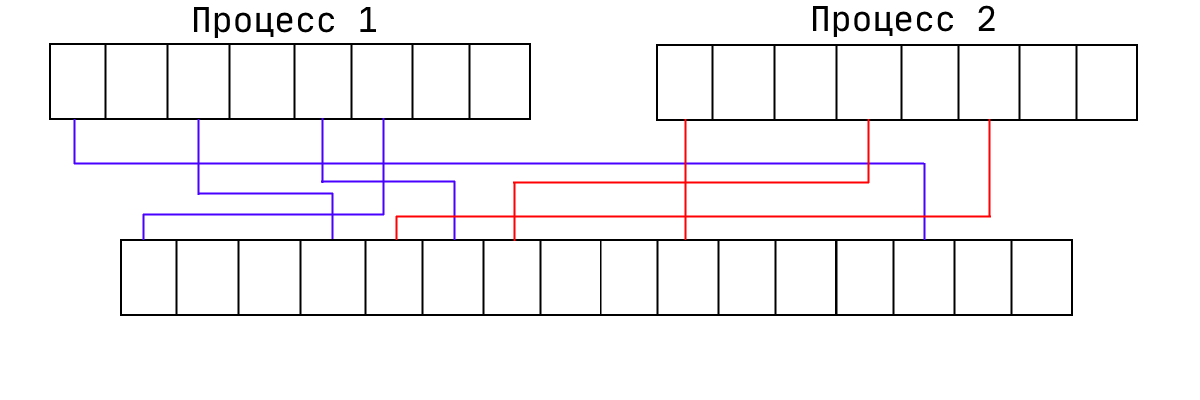
\includegraphics[scale=0.5, ]{virtual_memory1.png}
	\\Физическая память делится на блоки по 4КБ, каждый из которых имеет адрес, кратный 4КБ. Эти блоки сопоставляются блокам виртуальной памяти процессов. Адрес, используемый программой до обращения к памяти, называется виртуальным адресом. Мы можем так настроить трансляцию адресов, что два блока виртуальной памяти будут ссылаться на один и тот же блок физической. Понятно, что ничего хорошего не выйдет. Также не обязательно сопоставлять все виртуальные адреса физическим, некоторые можно пометить как невалидные. Обращение к отсутствующей странице приводит к передаче управления операционной системы. Для описания такого сопоставления используются записи следующего вида:\\\\
	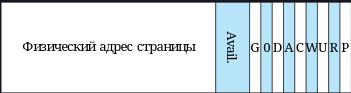
\includegraphics{virtual_memory_flags.png}\\
	В записях содержится информация о физическом адресе страницы, её валидности, разрешении на запись, привилегиях, работе с кэшем и т.д. Еще есть avail -- свободные биты для использования программой.
	\\\par Если хранить для каждой страницы такую запись отдельно, нам никогда не хватит памяти. Поэтому, в 32-х битном случае делают такую таблицу 1024х1024 (или дерево):\\
	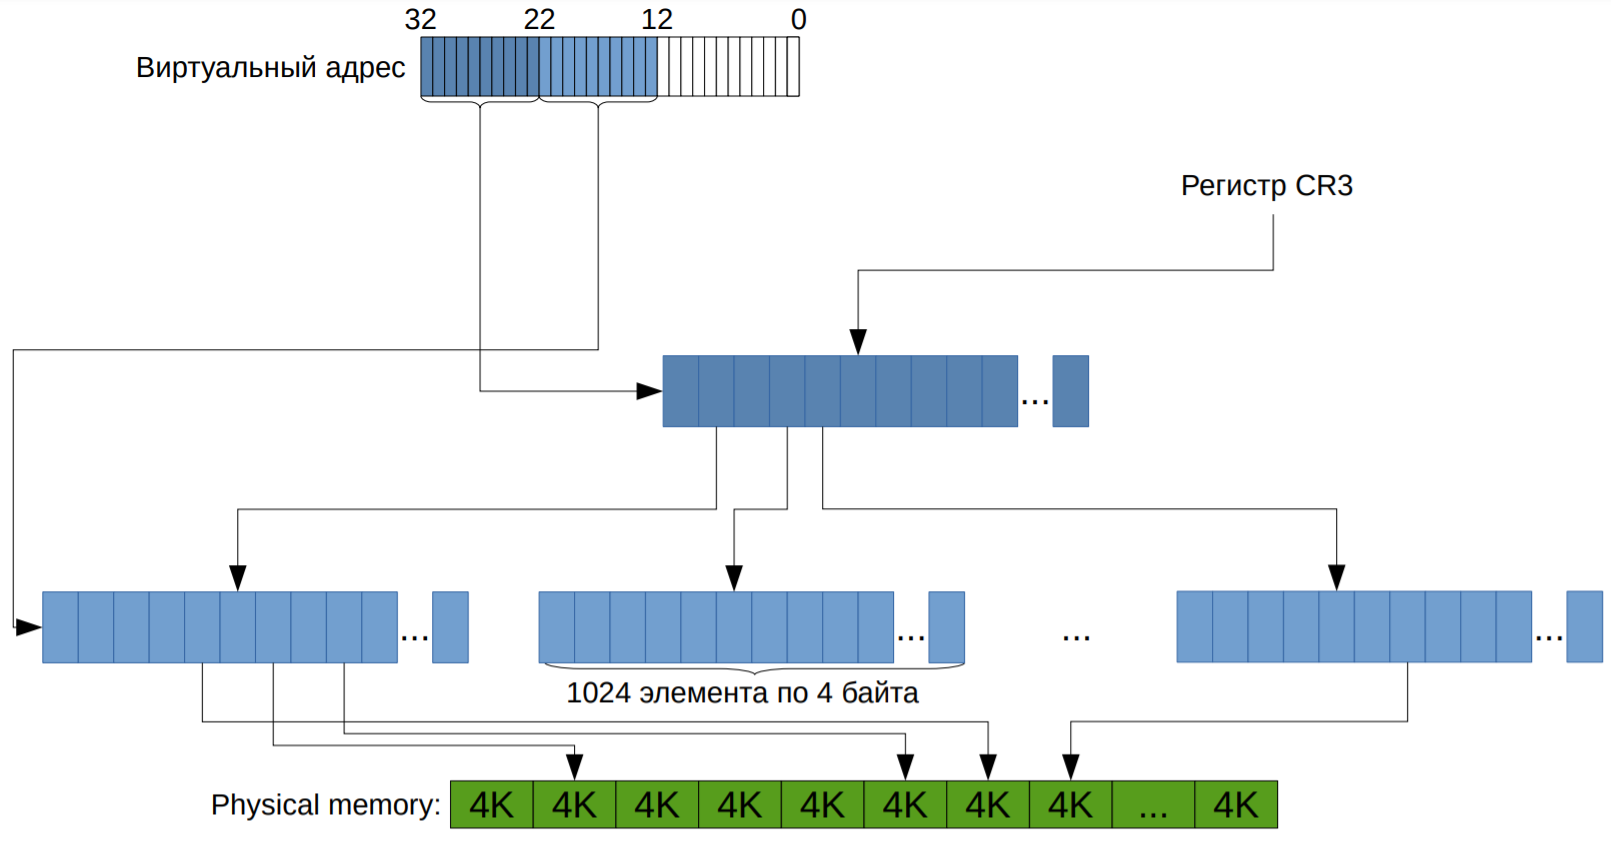
\includegraphics[scale=0.35]{virtual_memory_on_32.png}\\
	Верхний уровень называется каталог страниц. Первые десять битов адреса определяют позицию в каталоге. Вторые десять битов определяют уже сам номер страницы. Последние двенадцать используются для адресации внутри одной страницы. Подобная система не только хранит информацию о страницах компактнее, но также если есть невалидные 1024 страницы, идущие подряд, можно вообще для них ничего не хранить, а отметить их невалидными уже на верхнем уровне.
	\\\par В 32-х битных системах выбранные размеры очень хорошо сходятся. В 64-х битных уже плохо сходится. Там в страничной адресации используется больше уровней. При этом не все биты адреса используются для поиска в каталоге страниц, поэтому старшие белые биты по соглашению обязаны быть равны самому старшему желтому биту (см. картинку). Обращение к адресу, у которого это не выполняется, гарантировано приведет к ошибке. \\
	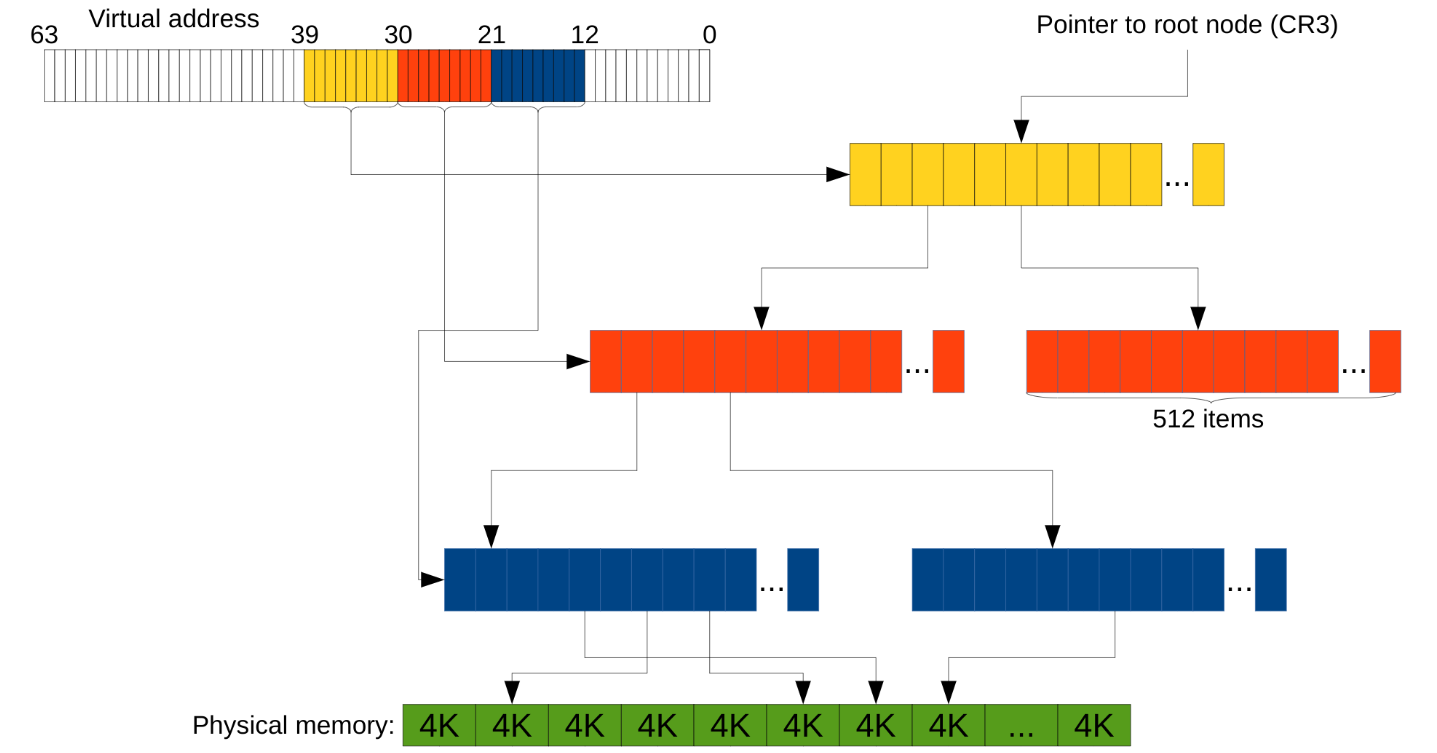
\includegraphics[scale=0.4]{virtual_memory_on_64.png}\\
	\par Как происходит выделение страниц для программы? Внтури мейна вызывается mmap, mmap запоминает, что должен выделить программе память, и выходит. Через некотрое время, когда мейн пытается обратиться к этой памяти, он наткнется на невалидную память и управление передастся операционной системе. Там посмотрят, что mmap обещал выделить память и обращение на самом деле валидное. Однако, просто так память отдать нельзя. Вдруг предыдущие процессы, которые ей владели, записали туда свои важные данные? Перед передачей памяти следующему процессу ее нужно почистить. Именно на это тратится большая часть времени при выделении страниц. Если же к запрошенной памяти не обращаться, она не будет почищена, и, следовательно, выделение будет быстрым.
	\\\par У страничной адресации есть несколько разных применений. Первое -- memory mapped files. Операционка как бы <<делает вид>>, что файл лежит в определенном месте в памяти. Благодаря этому этот файл можно подгружать не целиком, а постранично как обычную память.\\
	\textit{Замечание}. С помощью memory mapped files также можно достичь эффекта, когда виртуальной памяти больше физической. Если не хватает памяти, можно выкинуть какую-нибудь read-only страницу, продублированную на диске, и при необходимости прочитать ее снова. Для read-write страницы, в которую ни разу не писали, можно сделать то же самое. Для этого и предназначен бит Dirty.
	\par Еще одно применение -- shared memory. Две программы могут работать с одной и той же физической памятью, при этом в разной виртуальной памяти.
	\par Еще один способ сделать виртуальной памяти больше чем физической -- файл подкачки (swap file). Данные из страницы можно временно записать на диск и отдать страницу кому-нибудь другому, а в случае обращения вернуть страницу с диска.
	\par Также можно осуществить copy-on-write с помощью страничной адресации. Если нужно отредактировать маленькую часть большого файла, весь файл копироваться не будет, а можно скопировать только несколько страниц и отредактировать их. Через это, в частности, работают библиотеки.
	\\\textit{Замечание}. Можно посмотреть, сколько памяти использует каждая программа, с помощью process explorer. Память там описывается разными числами: virtual size -- общий размер памяти, с которой может работать программа, private bytes -- сколько памяти было выделено лично ей (private памятью, в отличие от shared, пользуется только один процесс). Working set -- объем памяти, к которому реально происходят обращения, а private working set -- понятно что.
	\\\par Немного про стек: на самом деле это всего лишь отмепленный кусок памяти в режиме read-write. Что произойдет, если мы случайно переполним его и выйдем за границу? У операционок обычно есть защита от этого: перед стеком резервируют одну страницу, которая никогда не бывает отмеплена и при обращении к ней происходит SIGSEGV. Программа, однако, может перескочить эту страницу и обратиться к памяти за ней, поэтому в линуксе недавно вместо страницы в 4КБ сделали размер этой защиты 1МБ. Стандартный размер стека 8МБ, поэтому попытка завести больше 1МБ локальных переменных в функции это редкий случай. На винде к этой проблеме подошли по-другому: стек -- это такая особая часть памяти, что page fault должен происходить на подряд идущих страницах, то есть если программа создала больше 4КБ локальных переменных, компилятор обязан сгенерировать код, который пройдет по всем страницам подряд до той, которая используется, чтобы наткнуться на guard page в случае переполнения.
	\subsection{Кэш}
	Рассмотрим два примера кода:
	\begin{minted}[tabsize=4, autogobble]{C++}
		// variant A
		char a[N][N];
		
		for (size_t i = 0; i != N; i++)
		    for (size_t j = 0; j != N; j++)
		        a[i][j] = 0;
		
		// variant B
		char a[N][N];
		
		for (size_t i = 0; i != N; i++)
		    for (size_t j = 0; j != N; j++)
		        a[j][i] = 0;
	\end{minted}
	В первом случае код будет работать намного быстрее благодаря кэшу. Дело в том, что скорость обращения к памяти намного хуже чем скорость арифметических операций. Для этого между процессором и оперативкой находится мини оперативка: кэш. Это устройство сохраняет несколько подряд идущих ячеек памяти, к которым идет обращение, в кэш-линии. Подробнее про кэши в курсе ЭВМ. Смысл примера в том, что в варианте А обращения к памяти идут последовательно, а значит каждое следующее обращение скорее всего попадет в ту же кэш-линию, что и предыдущее, а значит память в этом месте будет уже закэширована и обращение будет к кэшу, а не к памяти.
	\par Если процессор понимает, что обращения к памяти последовательные, он может заранее начать читать данные в кэш еще до обращения к ним. Это называется префетчинг.
	\\\par Обычный кэш кэширует по физическим адресам, но у нас есть виртуальная память. В таком случае для кэширования результатов трансляции из виртуального адреса в физический используется TLB кэш.
	\par Даже при наличии TLB кэша может случиться кэш-промах, и тогда придется проходить всё это дерево адресации из 4-5 уровней. В процессоре на этот случай есть оптимизация huge pages: специальный бит S указывает, что мы, находясь на красном уровне, не хотим спускаться дальше по дереву, а сразу искать большую страницу размером 2MБ. Из-за меньшего числа преобразований адреса мы экономим место TLB кэша. Также можно взять огромную страницу на еще более высоком уровне, тогда она будет размером 1ГБ.
	\subsection{Предсказание переходов}
	В упрощенном варианте работу процессора можно рассматривать как конвеер из нескольких этапов. Инструкции загружаются на конвеер последовательно. Следующая инструкция загружается, когда предыдущая проходит первый этап, и таким образом они движутся по конвееру. Здесь, однако, проблему создают условные переходы. Из-за них мы не знаем, какую инструкцию выполнять следующей, пока не посчитаем предыдущую команду полностью. Для этого процессор может попытаться угадать наличие перехода и сделать все необходимые инструкции в зависимости от этого, а в случае чего отменить их.
	\par Понятно, что если предсказание переходов плохо работает, это сильно замедляет программу. Например, если выполнение условия зависит от результата в линейном сдвиговом регистре с обратной связью, переходы будут плохо предсказываться, так как LFSR это почти рандом. Избавление от условного перехода ускорит код.
	\begin{minted}[tabsize=4, autogobble]{C++}
		// with branch
		unsigned lsb = lfsr & 1;
		lfsr >>= 1;
		if (lsb)
			lfsr ^= 0xB400;
		
		// no branch
		unsigned lsb = lfsr & 1;
		lfsr >>= 1;
		lfsr ^= 0xB400 * lsb;  // 0xB400 & -lsb even faster
	\end{minted}
	В коде выше можно подумать, что код с ветвлением будет работать медленнее. Однако, компилятор соптимизирует условный переход в первом коде, заменив его на команду cmovne. В общем случае ветвление действительно замедляет код. Если бы тело if было сложнее, компилятор бы не смог вставить cmovne.
	\\\textit{Замечание}. Компиляторы стараются как можно сильнее уменьшить количество зависимостей между последовательными инструкциями. Например, вместо умножения четырех интов последовательно, сгенерируется код, умножающий первые два, потом последние два и потом два полученных результата.
	\section{Введение в C++ (8 -- 9)}
	\subsection{Типы}
	Несколько моментов, касающихся обычных типов:
	\begin{itemize}
		\item char, signed char и unsigned char -- это три разных типа, в отличие от знакового и обычного инта. Проверить, являются ли типы разными, можно с помощью перегрузки.
		\item Битность некоторых типов, например long, зависит от ОС и битности системы. Поэтому, стоит использовать типы, у которых размер указан прямо в названии.
		\item Для индексации в массиве нужно использовать тип size\textunderscore t, размер которого зависит от битности системы.
		У size\textunderscore t есть знаковый вариант ptrdiff\textunderscore t, который нужен для разности указателей.
	\end{itemize}
	\par Кроме обычных типов также можно создать пользовательский тип, воспользовавшись enum class:
	\begin{minted}[tabsize=4, autogobble]{C++}
		enum class color {
			red,
			green,
			blue,
		};
		
		void draw(color);
		
		int main() {
			draw(color::green);
		}
	\end{minted}
	Преимущество enum перед обычными константами во-первых в том, что константы, обозначающие разные вещи, но имеющие все один тип, было бы легко перепутать, а еще enum как бы группирует константы и становится понятно, какие из них друг с другом связаны.
	\par По умолчанию все enum внутри себя содержат инты, но можно указать явно тип, на основе которого будут задаваться значения, а также в явном виде указать эти значения (например, если мы хотим сделать битовую маску):
	\begin{minted}[tabsize=4, autogobble]{C++}
		enum class color : uint64_t {
			red   = 1,
			green = 2,
			blue  = 4,
		};
	\end{minted}
	\textit{Замечание}. Помимо enum class есть обычные enum из С, для которых нельзя задать тип. Также для enum из С не надо квалифицировать имя (писать color:: в данном случае), а также они неявно конвертятся в числовые значения, а enum class так не может. Арифметические операции также не работают для enum class, но их можно перегрузить, использовав static cast.
	\subsection{Указатели, массивы и функции}
	Указатель -- это адрес переменной в памяти (виртуальной, естесственно). Помимо места указатель также хранит в себе информацию о типе. Доступ к элементу по указателю осуществляется с помощью разименовывания. Размеры всех указателей одинаковы и равны битности системы (так как это адрес). Если в программе используется указатель на переменную, эту переменную нельзя разместить в регистре, только в стеке или динамической памяти. Если время жизни переменной закончилось, указатель на нее нельзя разименовывать. Если у нас есть указатель на структуру, обращение к ее мемберам имеет сокращенную запись через оператор стрелку. Структура из char и int занимает 8 байт, а не 5, так как выравнивание требует, чтобы адреса были кратны 4. Структура из int и char тоже занимает 8 байт, так как выравнивание должно соблюстись также когда мы положим эту структурку в массив.
	\\\par Массивы и указатели это разные типы, но у них есть неявное преобразование из массива в указатель. Такая конверсия берет указатель на первый элемент массива. Дело в том, что сишные массивы не копируются, поэтому при передаче массива в функцию тип аргумента неявно приводится к указателю, это называется decay. Из-за всех этих неудобств вместо сишных массивов лучше использовать std::array. С указателями на элементы массивов можно делать арифметику указателей: прибавление и вычитание числа, сравнение, разность указателей.
	\\\par Немного приколов синтаксиса:
	\begin{minted}[tabsize=4, autogobble]{C++}
		int* ptr;       // pointer to int
		int arr[10];    // array of 10 ints
		int* arr[10];   // array of 10 pointers to int
		int* (arr[10]); // same as previous
		int (*arr)[10]; // pointer to array of 10 ints
	\end{minted}
	Чтобы правильно читать такие штуки в общем случае, нужно помнить, что суффиксные деклараторы, как и операторы, имеют больший приоритет.
	\\\textit{Замечание}. Любые, даже самые сложные типы, можно легко тайпдефать:
	\begin{minted}[tabsize=4, autogobble]{C++}
		// how to typedef this?
		int *** (*** (*** xyz[10][20][30]) [40][50][60]) [70][80][90];
		// xyz -> type
		typedef int *** (*** (*** type[10][20][30]) [40][50][60]) [70][80][90];
		type xyz;
	\end{minted}
	\par Функции довольно похожи на массивы, к ним тоже можно обращаться по указателю:
	\begin{minted}[tabsize=4, autogobble]{C++}
		void print_foo() {
		    std::cout << "foo\n";
		}
		
		int main() {
			void (*func)();
			func = &print_foo;
			func();
		}
	\end{minted}
	\subsection{Lvalue и rvalue}
	Каждое выражение является либо lvalue, либо rvalue. Rvalue -- временный объект, который не может стоять слева от знака присваивания, например 2 + 2. Lvalue это, например, имя переменной.\\
	\textit{Замечание}. Временные объекты (те, у которых нет имени) живут до перехода на следующую строчку.
	\\\par Немного синтаксических приколов (суффиксный и префиксный инкремент принимают lvalue, присваивание правоассоциативно):
	\begin{minted}[tabsize=4, autogobble]{C++}
		a++++; // error, a++ is rvalue
		++++a; // ok, ++a is lvalue
		+++a;  // same as ++(+a), error (+a is rvalue)
		++a++; // same as ++(a++), error (a++ is rvalue)
		a = 5 = 6;   // same as a = (5 = 6), error
		(a = 5) = 6; // ok
	\end{minted}
	\subsection{Константы}
	Рядом с типом можно написать const: это означает, что переменную нельзя менять. Как в таком случае работают указатели? Они, на самом деле, сохраняют информацию о константности, и при разименовывании в них нельзя писать.
	\begin{minted}[tabsize=4, autogobble]{C++}
		int const PI = 3;
		int* q = &PI; // error, wrong type
		int const* p = &PI; // ok
		*p = 4; // error, pointer to const
	\end{minted}
	\section{Компиляция программ (10 -- 12)}
	Обычно программа компилируется командой g++, но сама команда ничего не делает, только запускает другие команды. На самом деле процесс компиляции состоит из нескольких этапов.
	\\\par Первый этап -- \textbf{препроцессирование}. На этом этапе раскрываются директивы препроцессора (то что начинается с решетки, например include) и подставляются в код. Обычно файлы, полученные препроцессированием, имеют расширение .i.
	\\\par Второй этап -- \textbf{трансляция}. На этом этапе код компилируется в ассемблерный. Все основные оптимизации делаются на этом этапе.
	\\\par Третий этап -- \textbf{ассемблирование}. На этом этапе ассемблерный код компилируется в бинарник в каждом из файлов.
	\\\par Последний этап -- \textbf{линковка}. На этом этапе все единицы трансляции собираются в один исполняемый файл.
	\\\par Рассмотрим компиляцию двух единиц траснляции: 
	\begin{minted}[tabsize=4, autogobble]{C++}
		// a.cpp
		int main() {
			f(42);
		}
		
		// b.cpp
		#include <stdio.h>
		
		void f() {
			printf("Answer: %d\n", a);
		}
	\end{minted}
	В этой программе ошибка, которая возникает на этапе трансляции. Первая единица трансляции ничего не знает про функцию f и не может проверить тип f, но в зависимости от типа аргумента в f ей нужно генерировать разный код, поэтому она не может скомпилироваться. Чтобы она знала о типе f, ей нужно написать в начале объявление функции f.
	\begin{minted}[tabsize=4, autogobble]{C++}
		// a.cpp
		void f(int);
	\end{minted}
	Еще один вариант, когда может понадобиться объявить функцию -- если ее тело находится ниже места ее использования. Это может быть необходимо, если у нас две вызывающие друг друга функции.
	\par Если в одной единице трансляции объявлена функция, а в двух других есть две реализации этой функции, произойдет ошибка линковки.
	\\\par Есть способ пометить функцию локальной, чтобы ее не было видно из других единиц трансляции. Для этого ее нужно пометить static. С глобальными переменными работают все те же правила.
	\begin{minted}[tabsize=4, autogobble]{C++}
		void f(int);        // declaration
		void f(int) {}      // definition
		
		static void f(int) {}
		
		extern int a;       // declaration
		int a;              // definition
		
		static int b;
	\end{minted}
	\textit{Замечание}. Main нельзя вызывать как функцию.\\
	\textit{Замечание}. Даже если ничего не написать в качестве значения глобальной переменной, она всё равно будет инициализирована при запуске программы.
	\\\par В языке С функции при компиляции сохраняли свои имена. В С++ они мэнглятся: к имени добавляются части, позволяющие определить, что это за перегрузка. Из-за этого могут возникнуть трудности с линковкой единиц трансляции, которые написаны на разных языках, так как программа на С ищет одно имя, а программа на С++ предоставляет другое. Чтобы сказать компилятору не мэнглить функцию, надо написать extern "C". Тогда она получит имя по правилам языка С, но ее нельзя будет перегружать.\\
	\textit{Замечание}. Мэнглинг имен учитывает типы аргументов, но не учитывает возвращаемое значение (в GCC).\\
	\textit{Замечание}. В библиотеках, которые пришли из С, написан extern "C".
	\\\par Любопытный файл: если нам нужна функция printf, нам не обязательно инклюдить сишный хэдер, а достаточно написать extern "C" и объявление printf, и это будет работать. Хэдеры -- это файл с расширением .h, которые в процессе компиляции за единицу трансляции не считаются, а их содержимое подставляется туда, где их заинклюдили. Дело в том, что хэдеры содержат только объявления функций, а сами функции подключаются вместе с библиотекой на этапе линковки. Например, ключ -lc при линковке говорит <<линкуйся с сишной стандартной библиотекой>>. На самом деле, по такому принципу работают почти все хэдеры: в них содержатся только объявления функций, а сами функции  находятся в соответствующем cpp файле. При этом те файлы, которые хотят использовать функции, должны инклюдить хэдер, а не cpp. Если по ошибке заинклюдить cpp, получется ошибка multiple definitions очевидно почему (тело из cpp подставится в еще один файл и будут два определения).
	\\\textit{Замечание}. Для инклюда используются два варианта синтаксиса: <<ёлочки>> и "лапки" (официальное название, да). Ёлочки (треугольные скобки) ищут во всех каталогах и нужны для инклюдов из, например, стандартной библиотеки. Лапки (кавычки) ищут в текущем каталоге.
	\par Писать определения функций в хэдерах тоже плохо, так как потом если этот хэдер заинклюдят несколько файлов, во все из них вставится определение одной и той же функции и мы проиграем.
	\\\par В отличие от функций и переменных, структуры не участвуют в линковке. Они могут влиять на генерируемый код в плане всяких смещений в памяти, но сами по себе код не генерируют (имеются в виду структуры без методов), поэтому их считают декларациями. Их обычно пишут в хэдерах. Что если у нас есть структура x в b.h, c.h и d.h инклюдят b.h, а a.h инклюдит c.h и d.h? Получится multiple definition структуры x, так как она подставится два раза. Чтобы этого избежать, хэдеры пишут особым образом:
	\begin{minted}[tabsize=4, autogobble]{C++}
		// b.h
		#ifndef B_H
		#define B_H
		struct x {
			int a, b;
		};
		#endif
	\end{minted}
	Читается следующим образом: если имя макроса B\textunderscore H не определено, дефайним его и объявляем нашу структуру. Слишком громоздко, не так ли? Поэтому в компиляторе есть специальная прагма:
	\begin{minted}[tabsize=4, autogobble]{C++}
		// b.h
		#pragma once
		struct x {
			int a, b;
		};
	\end{minted}
	\par Рассмотрим такие <<рекурсивные>> структуры:
	\begin{minted}[tabsize=4, autogobble]{C++}
		// a.h
		#ifndef A_H
		#define A_H
		#include "b.h"
		struct a {
			b* bb;
		};
		#endif
		
		// b.h
		#ifndef B_H
		#define B_H
		#include "a.h"
		struct b {
			a* aa;
		};
		#endif
	\end{minted}
	Если бы не было ifndef, препроцессирование бы превратилось в бесконечный цикл, но с ifndef в b.h инклюд a.h раскроется в пустоту, так как A\textunderscore H уже задефайнен. Из-за этого у нас просто не будет структуры a в b.h. Чтобы починить ошибку, нужно сделать forward декларацию: вместо инклюдов написать объявление желаемой структуры.
	\begin{minted}[tabsize=4, autogobble]{C++}
		// a.h
		#ifndef A_H
		#define A_H
		struct b;     // the same in b.h
		struct a {
			b* bb;
		};
		#endif
	\end{minted}
	\par Вот мы написали в хэдере класс и инклюдим его в другие файлы, и в каждом файле у нас есть декларация этого класса. Но что если у нас в разных cpp файлах будут разные декларации одного и того же класса? Это считается ошибкой, однако простые классы до линковки не доживают, поэтому эту ошибку компилятор не ловит. Если всё же допустить такую ошибку, функция, работающая со структурой, будет думать что структура устроена по-другому, и из-за выравнивания будет неправильно с ней работать. 
	\\\par Небольшие функции компилятор не выделяет в ассемблерном коде, а сразу подставляет их тело в места использования, что позволяет применять оптимизации. Это называется инлайн. Однако есть проблемка. Компилятор не может сам инлайнить функции между единицами трансляции, так как на этапе, где происходит инлайн, единица ничего не знает о других единицах. Чтобы сказать компилятору инлайнить функцию в других единицах трансляции, нужно использовать специальное слово inline. Функцию определяют прямо в хэдере и дописывают к ней inline. При этом тело функции подставится во все места использования, но проблемы с multiple definition не будет, так как компилятор пометит такие функции особым образом, т. е. у них много определений, но все они одинаковые. Здесь нужно понимать, что инлайн функций -- это оптимизация, которую компилятор делает по своему желанию, а ключевое слово inline по сути говорит, что у функции может быть несколько определений в разных единицах трансляции, но все они одинаковые. При это компилятор может это соптимизировать, подставив эти определения прямо в код. Если же мы скажем, что определения одинаковые, но на самом деле они будут разными, получится Undefined Behavior.
	\\\par Здесь уже упоминалась директива define. Она подставляет вместо каждого вхождения одного токена другой токен, например \#define PI 3.14 подставит вместо каждого вхождения PI 3.14. Подстановка происходит на этапе препроцессинга. С дефайнами, однако, нужно быть аккуратнее: если кто-то попытается объявить переменную с таким именем, произойдет что-то очень нехорошее, причем ошибка может выглядеть очень странно. Лучше по возможности пользоваться константами. Если мы все-таки хотим использовать дефайн, но при этом чтобы он не поломал случайно другой код, можно написать дефайн перед кодом, в котором он будет использоваться, и в конце написать undef. Помимо обычных дефайнов можно еще использовать function-like дефайны:
	\begin{minted}[tabsize=4, autogobble]{C++}
		#define max(a, b) (a > b ? a : b)
	\end{minted}
	Function-like макрос нужно обернуть в скобки, потому что иначе может поломаться приоритет операций. Однако, такой макрос все равно может не работать, например если операнды являются тернарниками или вызовами функций, поэтому лучше вообще такими макросами не пользоваться.
	\par Еще есть макросы условной компиляции, такие как if, ifdef, ifndef, else, elif, endif. If позволяет включить в компиляцию кусок кода в зависимости от всяких вещей вроде операционной системы, ifdef эквивалентен if defined, ifndef соответственно if not defined.
	\section{Классы (13 -- 15)}
	\subsection{Инвариант класса, модификаторы доступа}
	В C при создании своего класса (структуры) функции, которые с ней работают, можно было писать только снаружи. Для того, чтобы как-то изменить объект, приходилось передавать указатель на этот объект в функцию, которая его меняла. В C++ появилась возможность писать функции для работы с объектами какого-то класса прямо в теле класса. В эти функции больше не надо передавать указатель на объект: можно считать, что у них есть неявный параметр *this, т. е. указатель на экземпляр класса. Внутри класса можно обращаться к мемберам через this-> (например если есть локальная переменная с таким же именем), а можно ничего не писать. Одна из главных причин написания функций внутри класса -- модификаторы доступа. Они позволяют указать, кто может видеть мемберы класса. Если пометить их как private, с ними смогут работать только внутренние функции класса. Поэтому есть правило: функции, которые не обращаются к приватным мемберам, принято делать внешними, в противном случае внутренними.\\\par 
	По какому принципу расставлять модификаторы доступа? Существует такое понятие, как инвариант класса. Это набор свойств, которые должны сохраняться во время работы с объектом, например, у класса рациональной дроби знаменатель всегда должен быть больше нуля. Тогда действует следующее правило: если изменение мембера или вызов какой-либо функции может нарушить инвариант класса, то этот мембер или функция должен быть private.\\
	\textit{Замечание}. Инварианты могут быть довольно неочевидными. Например, у класса строки, содержащей размер, capacity и указатель на буфер, есть инвариант, что указатель ссылается на выделенную память размера capacity, а так же что ячейки этой памяти с 0 по size - 1 проинициализированы.\\\par 
	Еще одна причина использовать модификатор private -- чтобы иметь возможность менять детали реализации, не ломая старые программы, которые на эти детали полагались. Например, в классе комплексного числа стоит скрыть мемберы, отвечающие за представление числа, на случай если оно поменяется.
	\\\textit{Замечание}. Разница между class и struct как раз в модификаторах доступа. В class по умолчанию всё private, в struct -- public.
	\subsection{Конструкторы и деструкторы}
	\par
	Существует проблема, связанная с инвариантами класса: при создании объекта, когда его поля не проинициализированы, инвариант может быть нарушен. Для этого существуют специальные функции -- конструкторы, которые вызываются при создании объекта:
	\begin{minted}[tabsize=4, autogobble]{C++}
		struct string {
			string(char const* str) {
				size = strlen(str);
				capacity = size;
				data = static_cast<char*>(malloc(capacity + 1));
				memecpy(data, str, size + 1);
			}
			private:
			char* data;
			size_t size;
			size_t capacity;
		};
	\end{minted}
	\par Чтобы вызвать конструктор, достаточно указать при создании объекта в круглых скобках аргументы конструктора. При этом, если не написать скобки, вызовется конструктор без аргументов, который называют дефолтным. То же самое будет если написать пустые скобки.
	\par Чтобы использовать объект, необязательно при создании давать ему имя. Например, можно сразу создать его как аргумент функции, вызвав конструктор:
	\begin{minted}[tabsize=4, autogobble]{C++}
		void foo(complex z) {}
		
		int main() {
			foo(complex(1., 2.));
			return 0;
		}
	\end{minted}
	\par Конструкторы, принимающие один параметр, играют особую роль: они называются converting конструкторы и используются для неявного приведения типов. Например, если у complex есть конструктор от double, следующие две строчки делают абсолютно одно и то же:
	\begin{minted}[tabsize=4, autogobble]{C++}
		foo(complex(42.));
		foo(42.); // calls converting ctor
	\end{minted}
	\textit{Замечание}. Если у функции foo будет перегрузка непосредственно от double, вторая строчка вызовет именно ее. Если будут перегрузки от двух типов, не являющихся double, но имеющих конструктор от него, компилятор не сможет выбрать между ними и произойдет ошибка.
	\\\par Иногда мы не хотим, чтобы конструкторы от одного аргумента использовались для неявных преобразований типов, например конструктор вектора от размера не должен работать как преобразование числового типа в vector. Чтобы этого избежать, конструктор надо пометить как explicit.
	\par Немного примеров явных и неявных приведений типов:
	\begin{minted}[tabsize=4, autogobble]{C++}
		string s("Hello");     // explicit
		foo(string("Hello"));  // explicit
		
		string t = "Hello";    // implicit
		foo("Hello");          // implicit
	\end{minted}
	\par Converting конструктор необязательно принимает строго один аргумент. Он может быть использован для конверсий если в него можно передать один аргумент, например, если у других аргументов есть значения по умолчанию. Следующий конструктор может быть использован и как конструктор от двух аргументов, и как converting, и как дефолтный:
	\begin{minted}[tabsize=4, autogobble]{C++}
		complex(double re = 0., double im = 0.) {
			this->re = re;
			this->im = im;
		}
	\end{minted}
	\par Мы можем преобразовывать не только другие типы в наш, но и наоборот с помощью operator:
	\begin{minted}[tabsize=4, autogobble]{C++}
		struct foobar {};
		
		struct convertible_to_foobar {
			operator foobar() const {}
		};
	\end{minted}
	Не стоит, однако, злоупотреблять такими конверсиями, и вот почему. Например, у нас есть конверсия из mytype в int и наоборот, и мы сравниваем на равенство объект mytype с объектом int. Тогда компилятор просто не сможет понять, что конвертировать: mytype в int или int в mytype.
	\\\par Помимо конструкторов есть еще деструкторы. Они вызываются, когда объект становится не нужен и удаляется, в частности, при завершении программы. В отличие от конструкторов, деструкторы всегда без параметров.
	\begin{minted}[tabsize=4, autogobble]{C++}
		~string() {
			free(data);
		}
	\end{minted}
	\textit{Замечание}. free может освобождать только память, выделенную malloc'ом.
	\\\par Небольшой момент, связанный с функциями класса: у функций класса есть неявный аргумент this -- указатель на наш объект, но мы можем хотеть передать его как константу, чтобы функция класса не могла его изменять. Поскольку аргумент неявный, написать ему тип const мы не можем, поэтому можно написать const после круглых скобок:
	\begin{minted}[tabsize=4, autogobble]{C++}
		void bar() const {}; // string const* this
	\end{minted}
	Это важно, если наш объект был создан как константа, так как в таком случае мы обязаны его не изменять.
	\subsection{Перегрузки операторов и ссылки}\par При написании своего класса, мы можем хотеть написать для него операторы, и было бы удобно, если бы для вызова этих операторов можно было использовать привычный синтаксис, например a + b вместо add(a, b). Для этого существуют перегрузки операторов:
	\begin{minted}[tabsize=4, autogobble]{C++}
		complex operator+(complex a, complex b) {
			return {a.real + b.real, a.imag + b.imag};
		}
	\end{minted}
	\textit{Замечание}. Эта перегрузка -- полноценная функция, и её можно вызывать соответствующе, написав operator+(a, b) вместо a + b.\\\par
	Но что будет, если мы захотим перегрузить оператор +=? Как нам передать туда объект, чтобы оператор мог его поменять и при этом мы могли бы написать стандартное a += b без амперсанда перед a? Для этого создали специальный тип: ссылочный.
	\begin{minted}[tabsize=4, autogobble]{C++}
		void operator+=(complex& a, complex b) {
			a.real += b.real;
			a.imag += b.imag;
		}
	\end{minted}
	\par Таблица сравнения указателей и ссылок: создание, обращение к объекту, обращение к мемберу и перенаправление указателя (для ссылок этого нет, они неизменяемые).
	\begin{minted}[tabsize=4, autogobble]{C++}
		pointer                 reference
		
		T* p = &a;              T& r = a;
		*p                      r
		p->foo                  r.foo
		p = &b;                 N/A
	\end{minted}
	\textit{Замечание}. Есть такое правило: когда вы инициализируете ссылку, она должна ссылаться на валидный объект, в отличие от указателя, который может быть nullptr.
	\\\par Ссылки также позволяют не копировать объект в функцию, поэтому их часто используют для больших объектов:
	\begin{minted}[tabsize=4, autogobble]{C++}
		complex operator+(complex const& a, complex const& b) {
			return {a.real + b.real, a.imag + b.imag};
		}
	\end{minted}
	\textit{Замечание.} Компилятор транслирует указатели и ссылки в один и тот же объект.
	\\\par Рассмотрим такую перегрузку оператора []:
	\begin{minted}[tabsize=4, autogobble]{C++}
		char operator[](size_t index) const {
			return data_[index];
		}
	\end{minted}
	Значение, полученное с помощью этого оператора, можно использовать как rvalue, но не как lvalue. Это логично, учитывая то, что возвращаемый char является копией символа строки. Чтобы можно было использовать его как lvalue, нужно возвращать ссылку на символ. Однако, этого недостаточно: нужно еще убрать const. Почему? Дело в том, что в функцию с const можно передать константную строчку, а затем получить ее символ как lvalue, то есть иметь возможность изменить символ константной строки, а это очень плохо.
	\begin{minted}[tabsize=4, autogobble]{C++}
		char& operator[](size_t index) {
			return data_[index];
		}
	\end{minted}
	Однако, возникла следующая проблема: теперь мы не можем обратиться к символу константной строки, просто чтобы на него посмотреть. Решение -- завести еще одну перегрузку для константных строк:
	\begin{minted}[tabsize=4, autogobble]{C++}
		char const& operator[](size_t index) const {
			return data_[index];
		}
	\end{minted}
	\par Выше был пример перегрузки оператора +=, который возвращал void. Однако, принято, чтобы этот оператор возвращал lvalue. Поэтому лучше будет написать его так: 
	\begin{minted}[tabsize=4, autogobble]{C++}
		complex& operator+=(complex& a, complex b) {
			a.real += b.real;
			a.imag += b.imag;
			return a;
		}
	\end{minted}
	\par Операторы * и -> тоже можно перегружать. Делается это так:
	\begin{minted}[tabsize=4, autogobble]{C++}
		struct pointer_to_mytype {
			my_type& operator*() const { return *inner };
			my_type* operator->() const { return inner };
			
			private:
			my_type* inner;
		}
	\end{minted}
	Почему -> возвращает указатель? Всё дело в том, что оператор -> является по сути унарным (то что стоит справа это не операнд, а просто имя). Поэтому в выражении p1->x компилятор сначала возьмет p1, применит к нему оператор ->, получит указатель, дальше опять применит к этому указателю -> и получит ->x.\\
	\textit{Замечание}. Если в операторе -> вернуть не указатель, а ссылку, при вызове оператора произойдет бесконечная рекурсия.\\
	\textit{Замечание}. Почему эти два оператора принимают константы, но при этом не возвращают константы? Причина в том, что константность здесь относится к переданному в оператор указателю, а не к объекту, на который он указывает. Поскольку оператор -> возвращает другой указатель, этот новый указатель не обязан быть константным. Если же убрать const, не получится разименовывать константные указатели.
	\subsection{Конструктор копирования и оператор =}
	Рассмотрим класс string и код, взаимодействующий с объектами этого класса:
	\begin{minted}[tabsize=4, autogobble]{C++}
		struct string {
			string() {
				data = strdup("");
				size = 0;
				capacity = 0;
			}
			
			string(char const* str) {
				size = strlen(str);
				capacity = size;
				data = static_cast<char*>(malloc(capacity + 1));
				memcpy(data, str, size + 1);
			}
			
			~string() {
				free(data);
			}
			
			private:
			char* data;
			size_t size;
			size_t capacity;
		};
		
		int main() {
			string a = "test";
			string b = a;
		}
	\end{minted}
	Такой код упадет с ошибкой из-за повторного free на уже удаленной памяти. Причина этого в том, что строки b и a хранят указатель на один и тот же буфер, и на выходе из программы, когда вызовутся их деструкторы, они будут удалять одну и ту же память. Как так вышло? Дело в том, что при отсутствии в классе копирующего конструктора и оператора присваивания, они создаются автоматически. В таком случае они будут просто копировать/присваивать все поля класса, и у нас будут два экземпляра строки с указателями на одну и ту же память. Здесь нарушился один из инвариантов нашего класса: два объекта не должны хранить указатель на одну память. Чтобы решить проблему, нужно переопределить конструктор копирования и оператор присваивания, чтобы они копировали/присваивали саму память, а не указатель.  
	\\\par Принципиальная разница между конструктором копирования и оператором присваивания заключается в том, что конструктор создает объект, а оператор присваивания меняет существующий объект. \\
	\textit{Замечание}. В конструктор копирования объект передается только по ссылке. Компилятор запрещает передавать его по значению, так как чтобы передать что-то по значению, нужно создать от него копию, а для этого понадобится копирующий конструктор.
	\\\par Рассмотрим такой код дефолтного конструктора:
	\begin{minted}[tabsize=4, autogobble]{C++}
		struct person {
			person() {
				name = "Eric";
				surname = "Addams";
			}
			
			private:
			string name;
			string surname;
		};
	\end{minted}
	Сколько аллокаций произойдет при вызове этого дефолтного конструктора? Кажется, что две, но на самом деле шесть. Во-первых, "Eric" это не строка, а строковый литерал, поэтому вызовется конструктор string. Во-вторых, собственно, оператор присваивания. Откуда третья аллокация? Как было сказано ранее, оператор присваивания изменяет уже существующий объект, поэтому name уже должен существовать на момент присваивания, но когда он был создан? Дело в том, что конструкторы перед выполнением кода в своем теле еще дополнительно вызывают дефолтные конструкторы всех мемберов класса. Поэтому перед присваиванием конструктор сначала создаст name как пустую строку, отсюда третья аллокация.
	\\\par Есть способ указать, какие именно конструкторы должны вызываться у мемберов класса перед заходом в конструктор самого класса:
	\begin{minted}[tabsize=4, autogobble]{C++}
		person() 
		: name("Eric")
		, surname("Addams")
		{}
	\end{minted}
	Это также работает в том случае, когда мы инициализируем мемберы переданными в конструктор параметрами:
	\begin{minted}[tabsize=4, autogobble]{C++}
		person(std::string const& name, std::string const& surname) 
		: name(name)
		, surname(surname)
		{}
	\end{minted}
	\textit{Замечание}. Из примера видно, что дефолтный конструктор должен по возможности избегать аллокаций (например в классе string нужно разрешить указателю на буфер быть nullptr для пустой строки). Обычно дефолтный конструктор вызывается, чтобы потом в этот объект что-то присвоить, и мы не хотим иметь здесь лишнюю аллокацию.
	\\\par Итого, существуют четыре функции, которые могут генерироваться автоматически: дефолтный конструктор, деструктор, копирующий конструктор и оператор присваивания. Сгенерированный деструктор ведет себя как деструктор с пустым телом: вызывает деструкторы всех мемберов в обратном порядке. Все функции кроме дефолтного конструктора генерируются в случае их отсутствия. Дефолтный конструктор генерируется в том случае, если не написан ни один другой конструктор (копирующий не в счет).
	\\\par Иногда нужно создать класс, для которого копирование и присваивание не определено, и при этом не хочется, чтобы существовали дефолтные функции для них, например класс, содержащий хендл файла. Тогда можно запретить соответсвтующие функции с помощью delete:
	\begin{minted}[tabsize=4, autogobble]{C++}
		file(file const&) = delete;
		file& operator=(file const&) = delete;
	\end{minted}
	\par Существует <<обратная>> к delete операция -- default. Это означает, что конструктор должен генерироваться автоматически. На первый взгляд кажется, что это избыточный синтаксис, но он служит для двух целей: во-первых, при отсутствии автогенерируемых функций, можно подумать, что про них просто забыли, тогда default -- способ показать, что их не стали писать сознательно, и то, что генерируется автоматически, нам подходит. Во-вторых, дефолтный конструктор не будет генерироваться при наличии других конструкторов, поэтому его можно заставить сгенерироваться таким способом.
	\begin{minted}[tabsize=4, autogobble]{C++}
		int32_range() = default;
		int32_range(int32_range const&) = default;
	\end{minted}
	\subsection{Создание с помощью new}
	Иногда нам не подходит то время жизни объекта, которое мы можем получить, используя временные объекты и локальные переменные, мы хотим создавать и удалять объект в тот момент, когда захотим. Для этого используется new:
	\begin{minted}[tabsize=4, autogobble]{C++}
		int* p = new int(42);
		delete p;
	\end{minted}
	Например, это может использоваться для узлов дерева, так как они не должны быть привязаны к стеку или какому-то месту в программе. New сначала выделяет память нужного размера с помощью operator new (о нем будет сказано позже), а потом на этой памяти вызывает конструктор объекта.
	\section{Исключения (15 -- 16)}
	\subsection{Работа с исключениями}
	Исключения -- удобный способ сообщить о том, что в программе произошла исключительная ситуация. Все другие способы это сделать, такие как установка флага или возврат кода ошибки, довольно сильно увеличивают объем кода, так как после каждой строчки, где потенциально могла произойти ошибка, надо проверять наличие этой ошибки, чтобы в случае чего выйти из функции. К тому же, если мы возвращаем код ошибки, это ограничивает нашу функциональность, так как мы не можем вернуть вместо этого что-то полезное.
	\par Работа с исключениями осуществляется с помощью конструкций throw и try-catch. Первая позволяет бросить исключение, вторая -- обработать его. При возникновении исключения код без try-catch остановит работу и передаст управление выше, пока не встретится блок catch, обрабатывающий это исключение. 
	\begin{minted}[tabsize=4, autogobble]{C++}
		void f() {
			if (true) {
				throw error();
			}
		}
		
		int main() {
			try {
				f();
			} catch (error const& e) {
				std::cout << "error\n";
			}
		}
	\end{minted}
	\textit{Замечание}. При возникновении исключения управление переходит наверх не моментально: сначала у функции, где выкинулось исключение, вызываются все дестркуторы локальных переменных в обратном порядке.
	\par Существует специальная конструкция, позволяющая поймать исключение люого типа: catch(...). Важный момент: не все исключения предназначены для того, чтобы их ловили, поэтому при использовании такой конструкции нужно обязательно пробросить исключение дальше с помощью throw с точкой с запятой. Эта специальная форма throw позволяет пробросить дальше текущее исключение, каким бы оно ни было.
	\begin{minted}[tabsize=4, autogobble]{C++}
		int main() {
			try {
				f();
			} catch (...) {
				std::cout << "f threw an exception\n";
				throw;
			}
		}
	\end{minted}
	\textit{Замечание}. При создании своего исключения надо наследовать его от exception. Также catch(...) слишком общая вещь, лучше ловить конкретный тип исключений, если он известен.
	\\\par Типичная ошибка, возникающая при работе с исключениями -- ловить их по значению. В таком случае создается лишняя копия.
	\begin{minted}[tabsize=4, autogobble]{C++}
		catch (std::runtime_error e) {} // extra copy
		catch (std::runtime_error const& e)
	\end{minted}
	Еще одна ошибка -- пробрасывание того же исключения с указанием его имени, тоже приводит к лишней копии.
	\begin{minted}[tabsize=4, autogobble]{C++}
		throw e; // extra copy
		throw;
	\end{minted}
	Последняя ошибка -- некоторые люди создают исключение через new как в Java. В таком случае это, во-первых, лишняя аллокация, во-вторых, ловить теперь нужно указатель, а не само исключение, и, в-третьих, этому исключению придется где-то сделать delete.
	\subsection{Механизм исключений}
	\par Что происходит в программе, когда мы хотим поймать исключение? На самом деле, если взять две почти идентичные функции, одна из которых дополнительно делает try-catch, для них сгенерируется одинаковый ассемблерный код. Из этого можно сделать вывод, что вход в try-catch является бесплатным. Такая стратегия реализации называется zero cost exception. Почему же тогда код с исключениями считается медленным, даже если само исключение не произошло? Рассмотрим такой код:
	\begin{minted}[tabsize=4, autogobble]{C++}
		a = 1;
		foo();
		a = 2;
		foo();
		a = 3;
	\end{minted}
	Если функция foo небросающая, компилятор знает, что a должно быть равно 3 в любом случае и может соптимизировать. В противном случае у него меньше возможностей для оптимизации, так как появляются новые случаи.
	\par Если внутри функции не генерируется код для try-catch, то как же тогда это работает? В ассемблерном коде генерируется таблица, которая сопоставляет место в функции, где произошло исключение, с соответствующим catch блоком.
	\par Если исключение всё же произошло, это довольно сильно замедляет программу. Первая проблема, замедляющая работу с исключениями, это lock contention. Когда бросается исключение, мы хотим знать последовательность вызовов функций, которая привела к этому исключению. Это делается с помощью специальных таблиц, которые говорят, как нужно раскручивать стек вызовов. Эти таблицы могут находиться в различных shared object'ах (загруженных библиотеках), поэтому unwinder'у приходится смотреть на все из них, а они могут еще динамически подгружаться. И если у нас при этом многопоточка, возникает как раз этот lock contention. Вторая проблема -- медленный unwinder. По сути, в unwinder'е находится вся языконезависимая поддержка исключений. Он должен уметь отвечать на запрос: в каком состоянии окажется программа после выхода из функции? Механизм исключений делает такие запросы, но дополнительно спрашивает, не нужно ли сделать в том или ином месте try-catch. Почему же unwinder такой медленный? Дело в том, что его могут вызвать на любой инструкции, в том числе и на тех, которые обращаются к памяти. Из-за этого у него есть ряд ограничений, например невозможность аллоцировать память, вследствие чего он не может использовать никакие структуры данных. Поэтому единственный способ для него понять, как раскручивать стек -- смотреть в файл, где это написано, но в этом файле данные оптимизированы не под то, чтобы их читал unwinder, а под то, чтобы они занимали меньше места. Поэтому unwinder тратит много времени на развертывание стека. Третья проблема -- поддержка resumable исключений. Это возможность при попадании в catch возобновить работу программы с того места, в котором произошло исключение. Однако, как мы знаем, при возникновении исключения вызываются все деструкторы, и здесь они не должны вызваться, чтобы мы могли продолжить работу программы. Поэтому приходится раскручивать стек вызовов дважды. Забавно, что сам C++ не позволяет писать resume, но для поддержки языконезависимых исключений должен его поддерживать.
	\subsection{RAII}
	Такой код создает утечку:
	\begin{minted}[tabsize=4, autogobble]{C++}
		int* p = new int(42);
		int* q = new int(43);
		
		delete q;
		delete p;
	\end{minted}
	Если второй new выкинет исключение из-за нехватки памяти, память, выделенная под p, так и останется неосвобожденной, что создаст утечку. На самом деле эта проблема касается не только утечек памяти: то же самое может произойти с незакрытыми файлами.
	\par Для решения этой проблемы применяется принцип RAII: Resource Acquisition is Initialization. Он гласит, что выделение ресурсов должно происходить только при инициализации (т. е. вызове конструктора). Это позволяет написать деструктор, который автоматически вызовется при возникновении исключения и освободит ресурсы, выделенные в конструкторе. Из этого понятно, что код выше некорректный с точки зрения RAII. Чтобы он стал корректным, нужно обернуть int* в структуру, для которой написать деструктор, вызывающий delete.
	\\\par RAII поелезен не только для исключений. Пусть мы хотим открыть файлы a, b и c при помощи fopen. Тогда если не открылся a, мы выходим из функции, если не открылся b, закрываем a и выходим, если не открылся c, закрываем a, b и выходим. Получается очень много лишнего кода. Если же использовать RAII, достаточно будет просто выйти из функции в каждом из этих случаев.\\
	\textit{Замечание}. Такая же логика используется при инициализации мемберов в конструкторах: если какой-то из них при попытке создания бросил исключение, все уже созданные удаляются, исключение пробрасывается наверх и объект считается несозданным.
	\\\par Помимо malloc и free для аллокации и освобождения памяти могут использоваться operator new и operator delete. Они отличаются тем, что operator new при нехватке памяти бросает исключение, а не возвращает nullptr, а так же он, в отличие от malloc, определен для случая, когда ему передают размер 0. Важно помнить, что если память была выделена с помощью malloc, освобождать ее надо именно с помощью free, а если она была выделена operator new, нужно использовать operator delete. Внутри operator new конечно может быть реализован через malloc, но полагаться на это нельзя, так как это implementation defined.
	\subsection{Гарантии безопасности}
	Рассмотрим такой код для оператора присваивания:
	\begin{minted}[tabsize=4, autogobble]{C++}
		string& operator=(string const& rhs) {
			if (&rhs == this) {
				return *this;
			}
			
			operator delete(data);
			data = static_cast<char*>(operator new(rhs.size + 1));
			size = rhs.size;
			capacity = rhs.size;
			memcpy(data, rhs.data, size + 1);
			return *this;
		}
	\end{minted}
	Представим, что operator new бросил исключение. Тогда мы не сможем выполнить присваивание, а data уже стерта, то есть неудачное присваивание испортит нам строчку. Что еще хуже, так это то, что у испорченной строчки в конце вызовется деструктор, который попытается освободить память второй раз. Мы хотим, чтобы в случае исключения во время присваивания строчка просто оставалась в исходном состоянии.
	\par Эта проблема решается с помощью swap trick: мы создаем временную копию нашей строчки с помощью констурктора копирования, а в конце свопаем нашу строчку с ней. Если копирование не удастся, у нас просто останется пустая временная строчка, которая благополучно удалится, а наша исходная строка не испортится.
	\begin{minted}[tabsize=4, autogobble]{C++}
		string& operator=(string const& rhs) {
			string(rhs).swap(*this);
			return *this;
		}
	\end{minted}
	\par Два примера кода для оператора присваивания, приведенные выше, демонстрируют различные гарантии безопасности исключений. Это своего рода контракт, который сообщает, на что может рассчитывать пользователь, если произойдет исключение (сохранится ли объект в валидном состоянии, не будет ли утечек и т. д.). Выделяют четыре типа гарантий:
	\begin{itemize}
		\item Nothrow -- функция не бросает исключения.
		\item Сильная гарантия -- в случае исключения объект останется в том состоянии, в котором был до входа в фукнцию (присваивание со swap trick дает такую гарантию).
		\item Слабая, или базовая гарантия -- если произошло исключение, объект может быть изменен, но должны сохраниться все его инварианты. Также не должны произойти никакие утечки ресурсов.
		\item Отсутствие гарантий.
	\end{itemize}
	\par Небросающими функциями чаще всего являются дефолтный конструктор, size, clear, begin, end, swap, деструктор.
	\\\par
	Существует модификатор, который позволяет указать, что функция не бросает исключения -- noexcept. Обычно его используют как есть, но есть специальный синтаксис, позволяющий указать условие, при котором работает noexcept.
	\begin{minted}[tabsize=4, autogobble]{C++}
		void foo() noexcept {}
		void foo() noexcept(cond) {}
	\end{minted}
	\par По умолчанию деструкторы все noexcept, но с помощью вышеупомянутого синтаксиса можно заставить их бросать исключения. Но что произойдет в таком случае? Проблема в том, что деструкторы могут вызываться в ответ на исключения, и если в них самих при этом произойдет исключение, непонятно, как должна вести себя программа в таком случае. В C++ это счиатется фатальной ошибкой и вызывается std::terminate. Еще одна причина никогда не бросать в деструкторе -- ограничения, накладываемые контейнером на хранящиеся в нём типы. Почти все контейнеры стандартной библиотеки требуют чтобы их элементы имели небросающий деструктор.\\
	\textit{Замечание}. Если у нас есть файловая структура, в деструкторе необходимо закрывать файл, но fclose может бросить исключение. Поэтому нам ничего не остается, кроме как вынести close отдельной функцией и писать ее в программе, когда файл становится нам не нужен.
	\section{Undefined behavior (17 -- 20)}
	\subsection{Введение и примеры UB}
	Рассмотрим такой код:
	\begin{minted}[tabsize=4, autogobble]{C++}
		void copy(char* dst, char const* src, size_t n) {
			for (size_t i = 0; i < n; ++i) {
				dst[i] = src[i];
			}
		}
	\end{minted}
	На первый взгляд кажется, что компиятор должен соптимизировать этот код, чтобы копирование было не побайтовым, а некоторыми порциями больше одного байта, ведь это эффективнее, и у нас есть типы, позволяющие хранить несколько байт. Однако, в сгенерированном ассемблерном коде можно найти побайтовое копирование. Зачем оно там? Дело в том, что компилятор в своих оптимизациях обязан учитывать все случаи, в том числе и тот, когда dst и src ссылаются на пересекающиеся области памяти. В таком случае говорят что указатели алиасятся. Понятно, что никто не будет использовать этот метод в таких целях, но язык дает возможность это сделать, а значит компилятор обязан это учитывать.
	\par Если слишком строго учитывать все подобные случаи, можно дойти до того, что компилятор не сможет сделать ни одной оптимизации. Например, можно завести функцию, которая принимает по ссылке short и long, и с таким подходом компилятор не оптимизирует даже это, так как ссылки могут ссылаться на одну область в памяти. Поэтому существует strict aliasing rule: правило, согласно которому с объектом определенного типа можно работать только используя указатель именно на этот тип. С учетом этого правила, компилятор имеет право полагать, что указатели на разные типы не алиасятся. Однако из этого правила есть исключения: char может алиасить любой другой тип и знаковые и беззнаковые типы алиасятся.
	\par Иногда мы можем гарантировать, что указатели не алиасятся, но компилятор этого не знает и не оптимизирует наш код. Чтобы заставить его оптимизировать, можно использовать ключевое слово restrict, которое говорит, что указатель не алиасится ни с каким другим.
	\begin{minted}[tabsize=4, autogobble]{C++}
		void sum(float* __restrict res, float const* arr, size_t n) {
			// ...
		}
	\end{minted}
	\textit{Замечание}. restrict отсутствует в C++.
	\\\par Что будет, если написать restrict, но передать алиасящиеся указатели? Произойдет так называемый undefined behavior. Это ситуация, когда результат программы непредсказуем и зависит от железа и других факторов. Примерами UB также являются: деление целочисленного типа на ноль, переполнение знакового целого числа, сдвиг на отрицательное число, разыменование nullptr. Последний пример является UB, так как в некоторых архитектурах адрес 0 может быть валидным адресом памяти, а еще бывает такое, что обращение к невалидному адресу памяти просто игнорируется, а не падает с SIGSEGV. А еще UB -- это сдвиг указателя на статический массив за край массива (исключение -- сдвиг на размер вправо, чтобы была возможность проходить циклом до последнего элемента).
	\begin{minted}[tabsize=4, autogobble]{C++}
		int arr[10];
		int* p = arr;
		int x;
		
		p = arr; // OK
		x = *p; // OK
		
		p = arr + 9; // OK
		x = *p; // OK
		
		p = arr + 10; // OK
		x = *p; // UB
		
		p = arr + 11; // UB
		p = arr - 1; // UB
	\end{minted}
	\par Компиляторы вполне себе знают о существовании UB и могут это использовать. Например, если написать функцию, проверяющую, что число является максимальным значением int, как a + 1 < a, компилятор увидит, что тут переполнение знакового типа, и заменит на функцию, которая всегда возвращает ноль, так как UB имеет право выдать любой результат.
	\\\par Еще один пример UB -- запись в константу. При этом, если объект изначально был не const, мы сделали его const, а потом сняли константность и поменяли объект, это разрешенный код, хоть и не очень хороший. Но если мы с помощью const cast получили ссылку на объект, который изначально был const, и изменили его -- это UB. При этом могут быть такие варианты поведения как нормальная работа, как будто const'а нет, изменение константы ни к чему не приводит (она уже захардкожена компилятором во все места использования), а так же SEGSEGV (если константа попадет в read-only data в ассемблере). Компилятор может сделать и другие варианты.
	\\\par В C++ есть специальное ключевое слово -- \textunderscore\textunderscore builtin\textunderscore unreachable, которое сообщает компилятору, что какое-то место в коде не должно достигаться. Если оно достигнется, произойдет UB. Это позволяет компилятору оптимизировать код. Например, если известно, что значение enum в switch может быть только от 1 до 3, в default можно написать \textunderscore\textunderscore builtin\textunderscore unreachable, чтобы он просто не рассматривался:
	\begin{minted}[tabsize=4, autogobble]{C++}
		switch(c) {
			case color::red:
			puts("red");
			break;
			case color::orange:
			puts("orange");
			break;
			case color::yellow:
			puts("yellow");
			break;
			default:
			__builtin_unreachable();
		}
	\end{minted}
	\textit{Замечание}. Деление от сдвига на 2 отличается только на отрицательных значениях, поэтому, если мы для случая a < 0 напишем unreachable, компилятор спокойно заменит деление на сдвиг.
	\subsection{Санитайзеры и valgrind}
	Для отлова UB можно использовать различные санитайзеры. Например, если обращаться к некорректному адресу, программа не особо пояснит, из-за чего именно произошел SIGSEGV, но если запустить с address sanitizer, он скажет, где именно произошло обращение к памяти, приводящее к UB, и даже где эта память была выделена. Также этот санитайзер ловит double free. Вот некоторые типы санитайзеров:
	\begin{itemize}
		\item address -- при аллокации и освобождении памяти помечает память как доступную или запрещенную. На каждые 8 байт хранит shadow byte, который обозначает, сколько из этих 8-ми байт доступны для обращения.
		\item leak -- подмножество address, проверяющий утечки памяти
		\item memory -- проверяет неинициализированную память
		\item thread -- проверяет, чтобы разные потоки в многопоточке не работали одновременно с одними переменными
		\item undefined -- комплект из различных проверок
	\end{itemize}
	Отличие memory санитайзера от предыдущих -- он не может быть запущен на какой-то части кода, только на всём коде целиком. Иначе, если какой-то код будет писать в память, но не отмечаться у санитайзера, может произойти ложное срабатывание (санитайзер подумает, что там неинициализирована память). То же самое относится к thread санитайзеру.
	\\\par Еще один инструмент для отлова ошибок -- valgrind. Он декомпилирует уже готовый бинарник и вставляет туда проверки. Плюс valgrind по сравнению с санитайзерами в том, что он видит все системные библиотеки, так как работает с уже скомпилированным бинарником. Valgrind, как и санитайзеры, использует shadow память. Из минусов valgrind -- он может проверять далеко не все UB.
	\\\par UB может возникать не только в самой программе, но и на уровне библиотеки. Например, попытка использования lower bound на неотсортированном массиве или обращение за пределы вектора. Есть ключи, которые проверяют UB в стандартной библиотеке, но не ловятся санитайзерами. Например, обращение за край контейнера std::list с помощью выхода за итератор end должно считаться ошибкой (по стандарту инкрементить за end нельзя), но поскольку list в стандартной библиотеке зациклен, без ключа для проверки UB в библиотеках санитайзеры это не поймают. Еще один пример подобного рода -- обращение к элементу вектора, который влезает в capacity, но его индекс превышает size. С точки зрения языка с этим нет проблемы, так как там находится выделенная память под наше распоряжение (например после reserve), но выход за size в контейнере это плохо и UB.
	\\\par В таких ситуациях может возникнуть желание сделать что-то такое со своим собственным кодом: если какое-то состояние правильное с точки зрения языка, но на более высоком уровне нарушает логику, надо как-то дать об этом знать. И это плавно подводит нас к следующей теме.
	\subsection{Ассерты}
	Ассерт -- встроенный механизм языка, позволяющий включить в код проверку на какое-то условие, которое должно соблюдаться. В случае провала проверки он печатает сообщение об ошибке и вызывает std::abort. Assert не бросает исключение, так как он пришел к нам из С, где не было исключений.
	\begin{minted}[tabsize=4, autogobble]{C++}
		interval(int32_t low, int32_t high) : low(low), high(high) {
			assert(low <= high);
		}
	\end{minted}
	\par Пример кода с ошибкой:
	\begin{minted}[tabsize=4, autogobble]{C++}
		FILE* f = fopen("1.txt", "rb");
		assert(f != nullptr);
		// ...
		fclose(f);
	\end{minted}
	Ошибка здесь в том, что assert можно отключить по желанию, а проверять, что файл открылся, нужно всегда. Это не тот случай, где нужно использовать ассерт. Правило здесь следующее: корректная программа без ассертов должна оставаться корректной.
	\par Использование ассертов может сильно замедлить работу программы, так как некоторые проверки даже с точки зрения асимптотики могут быть хуже самого кода. Поэтому, чтобы люди не пытались оптимизировать условия в ассертах, их сделали отключаемыми.
	\par Почему свои собственные ассерты лучше писать с std::abort, а не с исключениями? Здесь, как и выше, работает правило, что поведение кода не должно меняться в зависимости от включенных/выключенных ассертов. Также можно легко написать код, который нарушает exception safety, и исключения от ассертов сделают отладку труднее. Помимо исключений и abort можно также использовать логирование. Оно, в отличие от исключений, не меняет поведение программы, но люди могут игнорировать этот вариант, в отличие от abort (нельзя игнорировать нарушение условия, из-за которого программа падает).
	\\\par Ассерты нужны для проверки инвариантов класса, а также предусловий функций. Однако, есть функции, которые гарантированно выдают какой-то результат на любых переданных аргументах. Тогда говорят, что у функции широкий контракт (например at у вектора гарантированно бросит исключение, если индекс выходит за границы). В противном случае говорят, что у функции узкий контракт (оператор квадратных скобок у вектора может принимать только корректные индексы, а иначе UB).
	\\\par Ассерты хороши, если код, который их содержит, вызывается, иначе они никогда не будут проверены. Существует техника fuzzing для проверки работы кода: на вход подаются случайные данные и отслеживается, не упали ли какие-то ассерты.
	\subsection{Оптимизации malloc}
	Напомню, что память для использования программой выделяется порциями по 4 Кб командой mmap (постранично), а освобождается с помощью munmap. Поговорим, как на основе этих команд работают malloc и free. Для маллоков в повседневной жизни 4 Кб это очень много, плюс отмапить страницу -- дело небыстрое, так как перед использованием всю страницу нужно занулить, а освобожденную страницу нужно инвалидировать на всех ядрах. Поэтому, очевидно, выделять страницу на каждый маллок не очень хорошо. Если замерить время, можно увидеть, что один маллок в среднем стоит в 5 раз дешевле одного кэш-промаха. На самом деле аллокаторы мапят страницу, а затем выдают её по кусочкам пока она не кончится. Для маленьких объектов используется что-то вроде односвязного списка, где в свободных узлах хранится служебная информация. Это позволяет эффективно выделять память.
	\\\par Помимо оптимизаций самих аллокаций используются оптимизации количества аллокаций. Например, оптимизация copy on write позволяет в контейнере делать аллокацию только при запросе изменения (или при запросе, потенциально приводящем к изменению, например неконстантный оператор квадратные скобки). Делается это следующим образом: в структуре хранится ссылка на буфер, который может быть общий для нескольких структур. Копирующий конструктор в таком случае просто привязывает к буферу новую ссылку. Если же понадобилось изменить данные, создается копия буфера, а от старого отвязывается ссылка, и если на него больше никто не ссылается, он удаляется. Такая оптимизация может быть полезна, если делается много копирований.
	\par Также есть оптимизация, позволяющая хранить маленькие объекты без динамического выделения памяти. Вместо ссылки на данные теперь хранится union из ссылки и статического массива. Минусы small object оптимизации в том, что при каждом обращении приходится проверять, является ли наш буфер статическим.
	\section{Шаблоны (21 -- 27)}
	\subsection{Специализации шаблонов}
	В отличие от С, в С++ появились шаблоны, которые позволяют не копипастить код, отличающийся только типами данных, а также удобно писать функции, возвращаемый тип которых зависит от типа аргументов. До появления шаблонов использовался тип void* (указатель, который нельзя разименовывать), в который кастилось значение для использования в функции, а затем кастилось обратно. Он плох тем, что нарушает type safety (например каст int $\rightarrow$ void* $\rightarrow$ string выкинет ошибку во время исполнения, а не на этапе компиляции). Также void* обычно слишком общий тип и можно обойтись более конкретным.\\
	\textit{Замечание.} Не стоит полагаться на reinterpret\textunderscore cast, т. к. это implementation defined.\par
	Также можно обойтись без шаблонов при помощи макросов, которые просто сгенерируют нужный код и подставят туда имя типа. Однако, во-первых, это может не сработать с типом вроде long long, а во-вторых для двух обозначений одного и того же типа (int32\textunderscore t и int) сгенерируется лишний код. Также здесь может быть проблема с ODR.\\\par
	Пример использования primary template:
	\begin{minted}[tabsize=4, autogobble]{C++}
		template <typename T>
		struct vector {
			void push_back(T const&);
			T& operator(size_t);
			T const& operator[](size_t) const;
		};
	\end{minted}
	Подстановка вместо T имени типа называется инстанциация.\\\par 
	Шаблонный код можно переопределить для какого-то конкретного типа. Это называется explicit specialization:
	\begin{minted}[tabsize=4, autogobble]{C++}
		template <>
		struct vector<bool> {
			//...
		};
	\end{minted}
	\textit{Замечание}. std::vector для bool на самом деле переопределен. Это позволяет хранить данные в нем компактнее, но из-за этого его функционал ограничен по сравнению с вектором для других типов.
	\\\par Существует еще partial specialization -- специализация, которая сама является шаблоном:
	\begin{minted}[tabsize=4, autogobble]{C++}
		template <typename U>
		struct vector<U*> {
			//...
		};
	\end{minted}
	Здесь для типа U создается структура, которая хранит указатели на тип U.\\
	\par Если в коде несколько partial специализаций, подходящих под какой-то набор типов, компилятор выберет наиболее специализированная. Если есть несколько одинаково подходящих, произойдет ошибка. Пример кода, порождающего ошибку:
	\begin{minted}[tabsize=4, autogobble]{C++}
		template <typename U>
		struct vector<int, U> {};
		
		template <typename V>
		struct vector<V, int> {};
		
		vector<int, int> a;
	\end{minted}
	Если добавить специализацию <int, int>, код заработает.\\\\
	Лирическое отступление: тип <<указатель на функцию>>.
	\begin{minted}[tabsize=4, autogobble]{C++}
		foo<int (*)(double)> j; // using function pointer in template
		int (*z)(double); // declaration of function pointer
	\end{minted}
	\par Типы, которые можно передавать в шаблон, зависят только от того, как они используются внутри шаблона. Например, сам по себе тип void можно передать в шаблон, но если там создается переменная этого типа, произойдет ошибка.
	\subsection{Шаблонные функции}
	\par Шаблоны можно использовать как для классов, так и для функций. Их использование очень похоже, за исключением того что для функций необязательно указывать тип, который подставляется в шаблон: он определится автоматически.
	\begin{minted}[tabsize=4, autogobble]{C++}
		template <typename T>
		T const& my_min(T const& a, T const& b) {
			return a < b ? a : b;
		}
		
		int a = my_min(1, 2);
	\end{minted}
	\par Partial специализаций для функций не существует. Вместо них (а также обычно вместо explicit специализаций) используются обычные перегрузки функций. Однако, бывает такое, что explicit и перегрузка работает по-разному:
	\begin{minted}[tabsize=4, autogobble]{C++}
		template <typename T>
		void foo(T*) {}
		
		#if 1
		template <>
		void foo<int>(int*) {} // foo(nullptr) doesn't work
		
		#else
		void foo(int*) {} // foo(nullptr) works
		
		#endif
	\end{minted}
	\par Объяснение примера: при вызове функции компилятор ищет сначала подходящую перегрузку и только потом проверяет наличие подходящей специализации. В первом варианте компилятор находит только одну перегрузку, принимающую T*, которая ему не подходит (неизвестно какой тип T должен получиться), и поэтому происходит ошибка. Во втором случае у него две перегрузки, и из них подходит вторая.
	\\\textit{Замечание}. Если функция принимает аргумент самого типа T (top-level deduction), выводимый тип не будет const, даже если переданный аргумент const, так как при передаче по значению создается копия и нет смысла делать ее const. С ссылочными типами то же самое, так как типы дедьюсятся на основе типа выражения, а они не бывают ссылочными, в отличие от типов переменных.
	\subsection{Шаблонные параметры}\par В качестве шаблонных параметров можно использовать не только типы, но и другую информацию, например число, обозначающее размер:
	\begin{minted}[tabsize=4, autogobble]{C++}
		template <typename T, size_t N>
		struct array {
			T elements[N];
		};
	\end{minted}
	Важно, что число должно быть известно на этапе компиляции.
	\\\par Все специализации работают для non-type шаблонных параметров, чтобы предоставить одинаковый интерфейс. В примере выше понадобится специализация, чтобы переопределить array размера 0.
	\par Non-type шаблонные параметры можно использовать и для функций. Например, следующая функция принимает ссылку на массив, хранящий элементы типа T, и имеющий размер N:
	\begin{minted}[tabsize=4, autogobble]{C++}
		template <typename T, size_t N>
		size_t size(T (&)[N]) {
			return N;
		}
	\end{minted}
	\par Помимо типов и чисел шаблонные параметры могут сами быть шаблонами. В примере ниже структура foo хранит переменные типа Container, в которые можно передать тип T.
	\begin{minted}[tabsize=4, autogobble]{C++}
		template <typename T>
		struct vector 
		{};
		
		template <template <typename T> typename Container>
		struct foo {
			Container<int> a;
			Container<float> b;
		};
		
		foo<vector> a;
	\end{minted}
	\par Шаблонные параметры, как и параметры функций, можно задавать по умолчанию. Например, в std::set есть второй шаблонный параметр, помимо типа элементов -- компаратор. По умолчанию это std::less для переданного типа.
	\begin{minted}[tabsize=4, autogobble]{C++}
		template <typename T, typename C = std::less<T>>
		struct set
		{};
	\end{minted}
	\subsection{Зависимые имена и проверка типов}
	\par Иногда возникают ситуации, когда нельзя определить как интерпретировать выражение, пока компилятор не поймет, чем являются имена в нем. Например так:
	\begin{minted}[tabsize=4, autogobble]{C++}
		(a)-b; // cast -b to type a or subtract b from (a)
		a<b&&c>d; // (a<b) && (c>d) or template parameter b&&c
	\end{minted}
	Если это происходит внутри шаблонного кода, у компилятора нет способа понять, чем является выражение, на этапе его разбора, так как типы еще не выведены. 
	\begin{minted}[tabsize=4, autogobble]{C++}
		template <typename T>
		void test(int b) {
			(T::nested)-b;
		}
		
		struct foo {
			typedef int nested;
		};
		
		struct bar {
			static int const nested = 42;
		}
		int main() {
			test<foo>(1); // (int)-1?
			test<bar>(1); // (42)-1?
		}
	\end{minted}
	В данном случае имя nested называется зависимым (зависит от переданного шаблонного параметра).
	\par Чтобы дать компилятору понять, как именно интерпретировать зависимое имя (как тип или значение), есть правило: перед именем, которое должно означать тип, пишут typename. Отсюда видно, что в примере выше вызов test с шаблонным параметром foo даст ошибку, так как не написан typename и компилятор ожидает значение. Аналогично, чтобы показать, что имя является шаблоном (как в примере с символами <>, если мы хотим интерпретировать его как шаблон), надо написать перед ним template.
	\\\par По стандарту компилятор обзан проверять типы, например запрещать попытки создания переменной типа void или разыменовывания того, что не является указателем, однако при использовании шаблонов он не может это сделать до выведения типов. Поэтому используется two-phase name lookup: сначала проверяются типы, которые известны на момент определения, а потом типы, которые станут известны после подстановки.
	\begin{minted}[tabsize=4, autogobble]{C++}
		template <typename T>
		void test(T x, int y) {
			*x; // error at instantiation time
			*y; // error at definition time
		}
		
		int main() {
			test(1, 2);
		}
	\end{minted}
	\subsection{Полиморфизм и компиляция шаблонного кода}
	\par Возможность функции работать со значениями разных типов называется полиморфизм. Если функции известно, с чем она работает, только в рантайме (например передача указателя на функцию компаратора в функцию сортировки) -- это динамический полиморфизм, а если на этапе компиляции (тот же пример, но реализованный через шаблоны) -- то статический. Преимущество статического полиморфизма в том, что у компилятора намного больше возможностей для оптимизации кода, однако он не позволяет выбирать тип в зависимости от результатов в рантайме. Еще одна проблема статического полиморфизма -- генерация большого количества кода, и, как следствие, увеличение времени компиляции.
	\par Лирическое отступление: если в коде есть цикл, внутри которого каждый раз проверяется одно и то же условие, компилятор выносит это условие наружу. Такая оптимизация называется loop unswitching.\\\par
	У шаблонного кода может возникнуть проблема, если объявление и реализация шаблонного метода находятся в разных единицах трансляции:
	\begin{minted}[tabsize=4, autogobble]{C++}
		// max.h
		template <typename T>
		T const& max(T const& a, T const& b);
		
		// max.cpp
		template <typename T>
		T const& max(T const& a, T const& b) {
			return a < b ? b : a;
		}
		
		// main.cpp
		#include "max.h"
		max(1, 2);
	\end{minted}
	Когда мы компилируем main.cpp, мы не можем сгенерировать код для max(int, int), так как в хэдере нет тела функции. Когда мы компилируем max.cpp, мы знаем тело функции, но не знаем, для каких типов генерировать код. Здесь ситуация похожа на ситуацию с inline, когда мы не можем инлайнить функцию, которая находится в разных единицах трансляции. Решение проблемы -- писать тело функции по месту объявления.\\
	\textit{Замечание}. Если функция max(int, int) вызывается в нескольких единицах трансляции, компилятор умеет инстанцировать её таким образом, чтобы не нарушить ODR. Для этого он помечает её как inline для линковщика и тот выбрасывает все лишние копии функции.
	\par Способ писать шаблонные функции в разных файлах все же есть. Если известно, для каких конкретно типов нужно сгенерировать код, можно в явном виде заставить компилятор это сделать с помощью явного инстанцирования:
	\begin{minted}[tabsize=4, autogobble]{C++}
		// max.cpp
		template <typename T>
		T const& max(T const& a, T const& b) {
			return a < b ? b : a;
		}
		
		template int const& max(int const& a, int const& b);
	\end{minted}
	\par В библиотеках часто бывает такое, что какой-то тип используется в шаблоне намного чаще остальных, и очень невыгодно инстанцировать его в каждом месте, где он используется, потому что линковщик все равно выбросит лишнее копии и нет смысла изначально их создавать. Для решения этой проблемы существует способ подавить инстанцирование с помощью слова extern:
	\begin{minted}[tabsize=4, autogobble]{C++}
		// <string>
		template <typename Char>
		struct basic_string {
			// ...
		};
		
		using string = basic_string<char>;
		extern template struct basic_string<char>;
		
		// string.cpp
		#include <string>
		template struct basic_string<char>;
	\end{minted}
	\textit{Замечание}. Проблема с разными единицами трансляции касается только модели компиляции, в которой нельзя заглядывать в другие единицы трансляции. В C++20 появились модули, и для них эта проблема неактуальна.
	\subsection{Incomplete type}
	\par Если объявить тип и определить его позже, в коде между объявлением и определением он будет считаться incomplete типом. Тип становится complete по закрывающей фигурной скобке определения, что позволяет запрещать различные рекурсивные структуры (они плохи тем, что по сути имеют бесконечный размер). Шаблонные рекурсивные структуры тоже запрещены, код ниже выдаст ошибку компиляции по причине incomplete type:
	\begin{minted}[tabsize=4, autogobble]{C++}
		template <typename T>
		struct foo {
			foo<T> x, y;
		};
		
		foo<int> z;
	\end{minted}
	\par Для шаблонов, в которых есть сложные зависимости, может быть важен порядок инстанцирования. Например, следующий код скомпилируется, но если внутри foo вместо type1 написать type2, возникнет ошибка использования incomplete типа:
	\begin{minted}[tabsize=4, autogobble]{C++}
		template <typename B>
		struct foo {
			typename B::type1 y;
		};
		
		template <typename T>
		struct bar {
			typedef int type1;
			foo<bar<T>> x;
			typedef int type2;
		};
	\end{minted}
	Это связано с тем, что при объявлении поля x bar это все еще incomplete тип, и компилятор, осуществляя инстанцирование сверху вниз, уже увидел type1, но не type2.
	\\\par Важный момент: компилятор инстанцирует функции по запросу, то есть он не будет инстанцировать функцию типом, если она с этим типом нигде не используется. Более того: он обязан так делать. По этой причине, например, можно пользоваться вектором, у которого есть оператор меньше, передав ему в качестве параметра тип без оператора меньше, если не вызывать этот оператор.
	\\\par Чтобы не перекомпилировать код лишний раз, создатели библиотек часто пользуются приемом под названием pointer impl, где хранят в структуре вместо мемберов указатель на другую структуру, которую определяют в файле .cpp:
	\begin{minted}[tabsize=4, autogobble]{C++}
		// mytype.h
		#pragma once
		#include <memory>
		
		struct mytype {
			struct impl;
			private:
			std::unique_ptr<impl> pimpl;
		};
		
		// mytype.cpp
		struct mytype::impl {
			int foo;
			int bar;
		};
		
		// main.cpp
		int main() {
			mytype x;
		}
	\end{minted}
	Однако, если попытаться скомпилировать код выше, причем именно main, и только в том случае, если в main используется mytype, произойдет ошибка: попытка удаления incomplete типа. Это связано с тем, что для mytype не определены implicit мемберы, такие как дефолтный конструктор и деструктор, и компилятор попытается сгенерировать их самостоятельно, в результате чего произойдет ошибка. Эта ошибка возникает из-за того, что implicit мемберы генерируются внутри определения mytype, где impl еще incomplete, а значит неясно, как вызвать на нем delete. Если же написать пустые конструктор и деструктор в .cpp, impl, определенный там же, уже не будет incomplete, и программа скомпилируется.\\
	\textit{Замечание}. Если написать пустой дефолтный конструктор, он всё равно будет что-то делать, а именно вызывать конструктор у всех мемберов, причем если произошло исключение, ему придется удалить все созданные мемберы и пробросить исключение дальше. Аналогично пустой деструктор будет вызывать деструктор от всех мемберов.
	\subsection{STL}
	STL -- это подмножество стандартной библиотеки, состоящее из контейнеров, алгоритмов, итераторов и другого.
	
	\par Контейнеры делятся на два типа: последовательности (vector, list, deque) и ассоциативные контейнеры (map, set, multimap, multiset и др.). В первых можно вставить элемент на конкретную позицию, во вторых контейнер сам решает, куда вставляется элемент.
	\par Что такое итераторы? Рассмотрим vector и list, точнее обход их элементов в цикле. И там и там цикл будет почти одинаковый, за исключением того, что в векторе мы будем ходить по индексам, а в листе по указателям на узел списка. Итераторы предоставляют инструмент, который позволяет сделать подобный код общим для разных контейнеров. По сути итератор это то, чем мы итерируемся в цикле: он ссылается на какой-то элемент, а также знает, какой элемент идет за ним. Таким образом, можно добавлять новые контейнеры с написанными итераторами, и все существующие алгоритмы будут для них работать.
	\par Итераторы делятся на разные категории в зависимости от количества операций, которые они поддерживают:
	\begin{itemize}
		\item Самым крутым является \textbf{random access iterator}: он позволяет переходить на n элементов вперед или назад, считать количество элементов между итераторами и прочее, причем вычислительная сложность этих операций должна быть O(1). Таким, например, является итератор вектора или обычный указатель. Его требуют различные сортировки и бинпоиски, которым надо прыгать через элементы.
		\item \textbf{bidirectional iterator}, в отличие от предыдущего, не может обращаться к произвольному элементу, но может перемещаться к предыдущему и следующему. Его требует, например, reverse (достаточно вспомнить, как он работает).
		\item \textbf{forward iterator} умеет еще меньше предыдущего: копирование, присваивание, разыменовывание и переход к следующему элементу. Некоторым алгоритмам, однако, этого достаточно, например partition и remove.
		\item \textbf{input iterator} умеет всё то же, что и предыдущий итератор, но ему разрешается пройти по последовательности только один раз и прочесть что-то из неё. \textbf{output iterator} делает то же самое, но записывает в последовательность. Они используются алгоритмом копирования.
	\end{itemize}
	\par У каждого контейнера есть итератор на первый элемент -- begin -- и итератор на элемент после последнего -- end. Можно также интерпретировать это так, что итераторы ссылаются между элементами, например, так удобно говорить в случае вставки или удаления элементов.
	\par Существуют еще reverse итераторы, которые двигаются в обратную сторону. У них есть метод base, который позволяет получить из reverse итератора обычный. Однако, здесь нужно думать об итераторе как будто он ссылается между элементами, потому что элемент reverse итератора не будет совпадать с элементом base.
	\\\par Как нам удалить все элементы, не подходящие под предикат, если мы имеем только итераторы? Если делать это самым тупым способом, просто вызывая erase на каждом плохом элементе, мы проиграем в асимптотике для вектора (но выиграем для списка). Для этого есть трюк remove\textunderscore if, который перегоняет все плохие элементы в конец и возвращает итератор на разделение между хорошими и плохими элементами. Это будет работать за линейное время для любого контейнера.
	\\\par До С++20 в сортировку приходилось передавать и begin, и end, так как она знала только итераторы и не умела брать нужные итераторы по контейнеру. В C++20 сделали std::ranges::sort, который принимает только контейнер и сам берет у него begin и end. Также в С++20 добавили концепты, которые позволяют наложить ограничения на тип в шаблоне.
	\\\par При выборе между стандартными алгоритмами и своими форами следует отдавать предпочтение первым, так как это делает код читабельнее (вместо непонятных форов название алгоритма, который понятно что делает).
	\subsection{Traits}
	Рассмотрим поподробнее случай, когда нам могут понадобиться ограничения на шаблоны:
	\begin{minted}[tabsize=4, autogobble]{C++}
		template <typename T>
		struct vector {
			void assign(size_t n, T const& element);
			
			template <typename Iterator>
			void assign(Iterator first, Iterator last) {
				// ...
			}
		};
		
		void test() {
			vector<int32_t> v;
			v.assign(10, -1);
		}
	\end{minted}
	В данном примере вместо каста к size\textunderscore t выберется перегрузка с итераторами, потому что Iterator здесь всего лишь обозначение, а не реальный итератор. Как же дать компилятору понять, что в качестве итератора нам нужен тип, обладающий нужными характеристиками?
	\par Первый способ -- использование associated type. Например, у всех контейнеров есть associated type iterator, а у самих итераторов value type.
	\begin{minted}[tabsize=4, autogobble]{C++}
		template <typename T>
		struct vector {
			using iterator = T*;  
		};
		
		template <typename T>
		void test() {
			typename vector<T>::iterator it;
		}
	\end{minted}
	Этот способ плох тем, что он не позволяет использовать типы, у которых нет этого associated type, но которые, тем не менее, могут использоваться с такими же целями, например указатель прекрасно может быть использован в качестве итератора, но у него нет value type. Чтобы это исправить, используют traits:
	\begin{minted}[tabsize=4, autogobble]{C++}
		template <typename Iterator>
		struct iterator_traits {
			using value_type = Iterator::value_type;
		};
		
		template <typename T>
		struct iterator_traits<T*> {
			using value_type = T;  
		};
	\end{minted}
	В стандартной библиотеке есть куча трейтов, например is\textunderscore pointer, который обычно равен false, а для указателей равен true. Также можно писать свои трейты.
	\\\par Допустим мы пишем копирование для типов, которое вызывает у элементов контейнера конструкторы. Однако, для достаточно простых типов, таких как int, можно просто использовать memcpy. Нам хотелось бы опознавать случаи, когда memcpy достаточно. Наивно мы можем просто проверить нужный трейт с помощью ифа, но, например, если от этого трейта зависит вызов функции, которая в случае невыполнения трейта может отсутствовать, например разность итераторов, если они не random access, код просто не скомпилируется, хоть плохие итераторы в этот иф не зайдут. Чтобы обойти это, используется tag dispatching:
	\begin{minted}[tabsize=4, autogobble]{C++}
		template <bool Val>
		struct bool_const {};
		
		template <typename T>
		T* copy_impl(T const* first, T const* last, T* out_first, bool_const<false>) {
			// without memcpy
		}
		
		template <typename T>
		T* copy_impl(T const* first, T const* last, T* out_first, bool_const<true>) {
			// with memcpy
		}
		
		template <typename T>
		T* uninitialized_copy(T const* first, T const* last, T* out_first) {
			return copy_impl(first, last, out_first, 
			bool_const<std::is_trivially_copyable_v<T>>());
		}
	\end{minted}
	Мы создали тип, шаблонную структурку bool\textunderscore const, которая имеет разный тип в зависимости от булевого значения, и передаем её в функцию impl, чтобы по ней выбрать перегрузку, а основная функция просто перевызывает impl, передавая ей тот тип структурки, который соответствует is\textunderscore trivially\textunderscore copyable для типа. Структурка здесь играет роль тэга: мы разносим две ветки ифа на разные функции, и она отвечает за то, какую перегрузку выберет компилятор. Однако, есть и другой способ: можно пометить одну из веток constexpr, чтобы при компиляции в коде осталась только одна ветка (напомню, что constexpr обозначает неизменяющееся выражение, значение которого известно на момент компиляции).
	\begin{minted}[tabsize=4, autogobble]{C++}
		if constexpr (std::is_trivially_copyable_v<T>) {
			// memcpy
		} else {
			// no memcpy
		}
	\end{minted}
	\subsection{SFINAE}
	Рассмотрим функцию, которая принимает контейнер и указатель на него, и у нее есть перегрузка для массивов:
	\begin{minted}[tabsize=4, autogobble]{C++}
		template <typename C>
		void do_something(C& c, typename C::iterator pos) {}
		
		template <typename T, size_t N>
		void do_something(T (&c)[N], T* pos) {}
		
		int main() {
			int a[10];
			do_something(a, a + 5);
		}
	\end{minted}
	Обратим внимение, что для массива задедьюсятся обе перегрузки, но при попытке подставить в первую произойдет ошибка: попытка взять итератор у обычного массива. Однако, этот код всё равно компилируется, потому что иначе любое использование второй перегрузки приводило бы к ошибке в первой. Чтобы этого не происходило, в языке сделали специальное правило: substitution failure is not an error (SFINAE). Имеется в виду то, что если при попытке подстановки параметров в функцию происходит ошибка, компилятор не должен кидать ошибку, а должен просто не рассматривать эту перегрузку. С помощью абъюза SFINAE можно переделать наш пример с копированием:
	\begin{minted}[tabsize=4, autogobble]{C++}
		template <bool C, typename T = void>
		struct enable_if {};
		
		template <typename T>
		struct enable_if<true, T> {
			using type = T;
		};
		
		template <typename T>
		typename enable_if<!std::is_trivially_copyable_v<T>, T*>::type
		uninitialized_copy(T const* first, T const* last, T* out_first) {
			// ...
		}
		
		template <typename T>
		typename enable_if<std::is_trivially_copyable_v<T>, T*>::type
		uninitialized_copy(T const* first, T const* last, T* out_first) {
			// ...
		}
	\end{minted}
	Здесь при выборе перегрзуки выбирается тот случай, когда у enable if получилось взять type (только если выражение, отвечающее за bool в enable if, равно true).
	\\\par Всё это конечно ужасные костыли, теперь всё это делается очень быстро и красиво с помощью концептов.
	\subsection{Variadic templates}
	Иногда мы хотим использовать шаблон, в котором не какое-то конкретное число параметров, а сколько передадут. Например std::tuple может быть создан для произвольного числа параметров. Также есть функции, которые хотят принимать n аргументов, например printf. В С можно было написать произвольное число аргументов с помощью трех точек, но это было абсолютно не типобезопасно, то есть можно было передать туда любой тип. В отличие от printf, std::format использует variadic templates и типобезопасен. Вот пример синтаксиса variadic шаблона:
	\begin{minted}[tabsize=4, autogobble]{C++}
		template <typename... T>
		struct mytype {
			std::tuple<T...> x;
		};
		
		mytype<> z;
		mytype<int> x;
		mytype<char, int*> y;
	\end{minted}
	Этот не очень интеллектуальный пример просто создает структурку с произвольным количеством типов и сует эти типы в tuple.\\
	\par Пример, как можно реализовать tuple с помощью variadic template:
	\begin{minted}[tabsize=4, autogobble]{C++}
		template <typename... T>
		struct tuple;
		
		template <typename C, typename... Rest>
		struct tuple<C, Rest...> {
			C current;
			tuple<Rest...> rest;
		}
		
		template <>
		struct tuple<> {};
	\end{minted}
	Разберемся что здесь происходит: мы объявляем структуру tuple, использующую variadic. Дальше пишем для нее специализацию на случай, если у нас есть хотя бы один тип: создаем структуру из него и tuple от остальных типов (такая своеобразная рекурсия). Рекурсию надо где-то закончить, поэтому пишем специализацию для пустого шаблона. На самом деле такая структура будет занимать больше памяти чем могла бы из-за хранения пустых структур. Понятно, что std::tuple реализован не так.\\
	\textit{Замечание}. Первые две строчки могут показаться бессмысленными, но primary template обязательно должен быть, потому что он дает компилятору понять, как выглядит шаблон, для которого написаны специализации.
	\\\par Немного о трех точках: это не часть имени, а обозначение, призванное показать, что именно мы раскрываем в последовательность. В примере выше, например, это последовательность типов в шаблоне, а вот пример, показывающий разницу между тем, куда ставить три точки:
	\begin{minted}[tabsize=4, autogobble]{C++}
		f(g(args...)); // f(g(a0, a1, a2, ...))
		f(g(args)...); // f(g(a0), g(a1), g(a2), ...)
	\end{minted}
	Можно использовать несколько шаблонных паков, например два пака одинаковой длины можно раскрыть как последовательность пар типов:
	\begin{minted}[tabsize=4, autogobble]{C++}
		template <typename U, typename V>
		struct zip;
		
		template <typename... UElems, typename... VElems>
		struct zip {
			using type = std::tuple<std::pair<UElems, VElems>...>;
		};
	\end{minted}
	Чтобы не делать функцию от n параметров рекурсивно (создавать функции от n, n - 1, n - 2 и т. д. аргументов) можно использовать fold expression по оператору, тогда пак раскроется с операторами между членами последовательности.
	\begin{minted}[tabsize=4, autogobble]{C++}
		// bad, n^2
		template <typename A0, typename... Rest>
		void println(A0 const& a0, Rest const& ...rest) {
			cout << a0 << " ";
			println(rest...);
		}
		
		// good, uses fold expression
		template <typename... Args>
		void println(Args const& ...args) {
			(std::cout << ... << args); // std::cout << a0 << a1 << ...
			std::cout << "\n";
		}
	\end{minted}
	\textit{Замечание}. Можно пользоваться правилом расстановки точек: когда что-то объявляется, точки пишутся слева от имени, а когда используется -- справа. Эта странность существует по той причине, что в С было занято обозначение имени с тремя точками после него в объявлении функции.\\
	\textit{Замечание}. К паку нельзя обращаться по индексу, так как в языке не существует compile time фора, но можно узнать иъ количество с помощью sizeof.
	\\\par Non-type шаблонные параметры тоже могут быть использованы в variadic template. Например, мы можем хотеть завести функцию, принимающую произвольное количество интов. 
	\begin{minted}[tabsize=4, autogobble]{C++}
		template<typename... Ts>
		requires (std::is_same_v<Ts, int> && ...) // fold expr
		void foo(Ts ...) {}
	\end{minted}
	\section{Namespaces (27 -- 28)}
	Чтобы понять, зачем нужны неймспейсы, достаточно посмотреть на библиотеку С, где их нет. Все функции там должны начинаться с названия библиотеки, потому что, если использовать короткое название, оно может пересечься с названием функции из другой библиотеки. Из-за этого имена функций становились очень длинными. Вот вариант использования неймспейсов:
	\begin{minted}[tabsize=4, autogobble]{C++}
		namespace cairo { // library "cairo"
			struct surface { // class "surface"
				void finish(); // short function name
				void flush();
			};
		}
	\end{minted}
	Неймспейсы используются для двух целей: предотвращение конфликта имен и структурирование кода (группировка классов и функций, служащих для одной цели). Неймспейсы могут вкладываться друг в друга. Самый верхний уровень имеет название global namespace. Внутри неймспейса имя ищется поднятием по уровням вложенности: сначала в самом неймспейсе, потом в том, в который он вложен и т. д. Чтобы обратиться к имени в неймспейсе, который не является нашим или предком нашего, используется ::.
	\begin{minted}[tabsize=4, autogobble]{C++}
		struct point{};
		
		namespace lib1 {
			struct surface{};
			
			void test1(surface, point) {}; // sees both surface and point
		}
		
		void test2(lib1::surface, point);
	\end{minted}
	Структуры в этом плане тоже являются своего рода неймспейсами, и обращаться к их содержимому снаружи тоже нужно через ::. Если мы хотим использовать имя не из текущего, а из глобального неймспейса, нужно написать перед ним ::.
	\par Неймспейсам можно присвоить псевдоним:
	\begin{minted}[tabsize=4, autogobble]{C++}
		namespace fs = std::filesystem;
		fs::path p;
	\end{minted}
	С помощью using можно указать, какое полное имя будет подразумеваться под его сокращенной записью:
	\begin{minted}[tabsize=4, autogobble]{C++}
		struct n {
			void foo(int);
		};
		
		using n::foo;
		
		void test() {
			foo(); // n::foo
		}
	\end{minted}
	Using также позволяет объединить перегрузки функций из разных неймспейсов. Также можно написать using namespace n, чтобы использовать имена из неймспейса n. Он по сути говорит: <<я сейчас нахожусь в глобальном неймспейсе, а еще поищи в неймспейсе n>>. Using namespace, в отличие от просто using, это не декларация, а директива. Она отличается тем, что если написать using namespace n1 и using namespace n2, где в n1 и n2 есть конфликтующие имена, но они никак не используются, ошибки не будет, потому что using namespace это просто указание где искать используемые имена. Также using декларация может не сработать, если ссылается на структуру, которая в коде объявлена ниже, а using namespace сработает. Третье отличие в следующем коде:
	\begin{minted}[tabsize=4, autogobble]{C++}
		namespace n {
			int const x = 1;
			int const y = 2;
		}
		
		namespace m1 {
			int const x = 10;
			int const y = 20;
			
			namespace m2 {
				using n::x;
				using n::y;
				
				void test {
					std::cout << x << " " << y;
				}
			}
		}
	\end{minted}
	Что выведет код, если запустить test? Он выведет 1 и 2, так как поиск имен поднимется из test выше, а там using декларация скажет ему искать в неймспейсе n и он остановится. А если вместо декларации написать директиву, это всего лишь даст ему понять, что в n тоже можно искать, и он все равно пойдет на уровень выше, где будет сказано, что x = 10, y = 20. Уровень, на котором подключится поиск в n, будет в наименьшем общем предке нашего неймспейса и указанного в using, то есть в глобальном неймспейсе.\\
	\textit{Замечание}. Имя, в котором используется ::, называется квалифицированным.
	\\\par Учитывая все вышесказанное про неймспейсы, непонятно, как мы, например, складываем и свопаем объекты своих собственные классов, потому что перегруженный оператор сложения находится внутри класса и непонятно, как использовать его снаружи без using. Чтобы это было возможно, существует правило ADL (Argument Dependant Look-up). Оно гласит, что при поиске имени функции нужно также посмотреть в местах, связанных с ее аргументами (в случае сложения в классах аргументов, которые складываются). ADL также ответственно за работоспособность шаблонного кода, так как приходится знать перегрузку различных функций для какого-то шаблонного типа, который находится в неймспейсе шаблонного кода.
	\\\par В С классы были локальными в пределах своей единицы трансляции, поэтому к ним нельзя было применить static. В С++ у классов появились различные неявные мемберы, которые генерирует компилятор. Эти мемберы являются полноценными функциями, поэтому, хоть классы и локальные, для двух классов с одинаковым именем эти функции тоже будут иметь одинаковое полное имя, а значит, нарушат ODR. Хочется помечать локальными не только функции, но и классы. Для этого придумали анонимные неймспейсы. Он пишется как обычный namespace, но без имени. Всё, что находится внутри, как бы является локальным.
	\section{Наследование (28 -- 30)}
	В С++ можно указать что один класс наследуется от другого, указав этот другой класс через двоеточие при объявлении. Класс, который наследуется, называется производным, а тот, от которого наследуются -- базовым. Работает это следующим образом: производный класс имеет свои мемберы, а также мемберы базового класса. Также можно приводить производный класс к базовому. Ссылка/указатель на производный класс приводятся к ссылке/указателю на базовый. Понятно, что мемберы, принадлежащие только производному классу, теряются.
	\begin{minted}[tabsize=4, autogobble]{C++}
		struct vehicle {
			std::string registration number;
		}
		
		struct bus : vehicle {
			std::string next_stop;
		}
		
		int main() {
			bus b;
			b.registration_number = "a";
			b.next_stop = "b";
			
			vehicle& v = b;
			std::cout << v.registration_number;
		}
	\end{minted}
	\par Мемберам в базовом и производном классе разрешается иметь одинаковые имена. Чтобы при наличии имени в производном классе обратиться по такому же имени базового класса, достаточно указать квалификацию имени (та штука :: если кто забыл). Ну или можно скастовать в базовый класс и обратиться по имени. Для функций и переменных эти правила одинаковые.
	\\\par Мы можем создать функцию, которая будет принимать ссылку на базовый класс, и передавать в нее все классы, которые от него наследуются. Здесь есть два определения: статический тип это тот, который написан в функции, то есть тип базового класса, а динамический тип это тот, который мы туда передаем (этот же тип или тип наследника). Обычные функции учитывают только статический тип, но есть особые функции, виртуальные, которые выбираются в соответствии с динамическим типом.
	\begin{minted}[tabsize=4, autogobble]{C++}
		struct vehicle {
			virtual void print_name() {
				std::cout << "vehicle\n";
			}
		}
		
		struct bus : vehicle {
			void print_name() {
				std::cout << "bus\n";
			}
		}
		
		void log(vehicle& v) {
			v.print_name();
		}
	\end{minted}
	В примере выше, если бы функция print\textunderscore name не была помечена как virtual, в функции log всегда бы вызывалась она, даже если был передан наследник vehicle. Но с virtual для выбора реализации print\textunderscore name используется динамический тип, то есть, хоть ссылка и на vehicle, при передаче bus выведется bus.\\
	\textit{Замечание}. Если в базовом классе есть виртуальная функция, соответствующую реализацию в наследнике можно пометить как override, но будет работать и без этого.
	\\\par Поговорим о том, как виртуальные функции устроены изнутри. Создается таблица, куда помещаются виртуальные функции. Базовый класс хранит указатель на эту таблицу. Затем для каждого наследника создается собственная таблица, в которой хранятся ссылки на все функции этого наследника. При создании объекта, наследующегося от базового класса, указатель на общую таблицу заменяется указателем на таблицу производного класса.\\
	\textit{Замечание}. Для нескольких уровней иерархии в таблицах хранятся оверрайды самого высокого уровня (т. е. реализация функции у базового класса, который ближе всех к нашему в иерархии, или наш собственный оверрайд, если он есть). Это называется final override. Также в таблицах хранится информация о динамическом типе, поэтому нам нужно создавать таблицу для каждого производного класса.
	\\\par Существует ошибка, которую можно сделать при работе с виртуальными функциями. Пусть у нас есть класс base с виртуальной функцией get\textunderscore name и его наследник derived, реализующий get\textunderscore name:
	\begin{minted}[tabsize=4, autogobble]{C++}
		// no mistake
		derived d;
		base& b = d;  // reference to derived with static type base
		b.get_name(); // dynamic type is derived so derived name
		
		// mistake
		derived d;
		base b = d;   // copy
		b.get_name(); // dynamic type is base because its another obj
	\end{minted}
	В первом случае мы просто взяли ссылку типа base на объект типа derived, то есть динамический тип будет derived и реализация метода вызовется соответствующая. Во втором случае произошло следующее: мы по сути пытаемся создать объект типа base с помощью копирования/присваивания другого объекта. Копирование/присваивание принимает ссылку на объект того же типа, но у нас очень удачно имеется каст ссылки derived в ссылку base. Таким образом происходит копирование, и динамический тип b будет base, а не derived. Эта ошибка называется slicing. Ее можно починить, если запретить классу base иметь конструктор копирования и присваивания. 
	\\\par Что происходит, когда мы хотим удалить объект, у которого статический тип не совпадает с динамическим? Допустим у нас есть указатель типа base на объект типа derived, и мы вызываем в конце работы delete на указателе. Тогда сначала вызовется деструктор, но он вызовется не у того класса из-за типа указателя, получится UB. Из этого очевидно следует, что деструктор надо сделать виртуальной функцией. Еще один вариант -- просто запретить вызывать деструктор не у того класса, сделав деструктор базового класса protected. В таком случае снаружи его не будет видно, но наследники смогут его перевызывать.
	\\\par Иногда, когда мы используем виртуальную функцию, писать ее реализацию для базового класса не имеет никакого смысла. Тогда мы можем пометить ее как абстрактную, написав вместо тела = 0. Класс, содержащий такие функции, называется абстрактным. Создавать объекты такого класса нельзя.
	\\\par С++ поддерживает множественное наследование: базовые классы нужно указать через запятую. Однако, с этим есть проблема: классы, от которых наследуется наш класс, распологаются в памяти друг за другом, поэтому при касте в любой кроме первого нам нужно сдвигать указатель. Например, посмотрим на код на С++ и сгенерированный ассемблерный код:
	\begin{minted}[tabsize=4, autogobble]{C++}
		// cpp
		struct base1 {
			int x;
		};
		
		struct base2 {
			int y;
		}
		
		struct derived : base1, base2 {};
		
		base1& to_base1(derived& d) {
			return d;
		}
		
		base2& to_base2(derived& d) {
			return d;
		}
		
		// asm
		to_base1(derived&):
		mov     rax, rdi
		ret
		to_base2(derived&):
		lea     rax, [rdi+4]
		ret
	\end{minted}
	Здесь хорошо виден этот сдвиг на размер нашего класса. В случае, если каст написан после объявления derived, но до ее реализации, компилятор не знает, от кого она наследуется, а значит и на какой размер двигать указатель. Для каста в base1 все сработает, так как там не надо сдвигать указатель, но для каста в base2 указатель тоже не сдвинется, хотя должен. Аналогично с кастами из base2 в derived. C-style каст не сможет распознать эту проблему на этапе компиляции и просто сделает неправильный каст. Поэтому нужно использовать static\textunderscore cast, который распознает ошибку на этапе компиляции.
	\begin{minted}[tabsize=4, autogobble]{C++}
		struct derived;
		
		derived& to_derived(base2& b2) {
			// return (derived&)b2; C-style cast causes an error in runtime
			return static_cast<derived&> b2; // compile error
		}
		
		struct derived : base1, base2 {};
	\end{minted}
	\par Пусть мы хотим иметь класс, который может хранить один из нескольких вариантов объектов, и в зависимости от варианта у него будут разные поля. Один из способов это сделать -- через union, а другой с помощью хранения базового класса, который, в зависимости от варианта, будет представлять собой какую-то свою реализацию.
	\\\par Еще немного про модификатор protected: как нам уже известно, мемберы, помеченные как protected, видны только производным классам. Однако, если внутри производного класса есть указатель на объект базового класса, мы не сможем обратиться к protected мемберу этого объекта базового класса. Однако, если есть указатель на объект производного класса, обратиться к его protected мемберу будет возможно.
	\begin{minted}[tabsize=4, autogobble]{C++}
		struct base {
			protected:
			int x;
		};
		
		struct derived : base {
			static void test(base* b, derived* d) {
				b->x; // error
				d->x; // ok
			}
		}
	\end{minted}
	Это сделано для того, чтобы protected не превратили в public с помощью наследования и перевызова.\\
	\par Чтобы понять, что от чего можно наследовать, применяют принцип подстановки Лисков. Он заключается в том, что все операции, применимые к базовому классу, могут быть разумно реализованы в производном классе. Функции, которые используют базовый тип, должны иметь возможность использовать вместо него объекты производного типа, не зная об этом.
	\par Бывает такая ситуация, что классы В и С наследуются от А, а класс D наследуется от В и С одновременно. Тогда мы можем хотеть два разных варианта: в первом варианте мы считаем, что В наследуется от своего куска А и С наследуется от другого куска А. По умолчанию в языке так и есть. Тогда, если мы попытаемся взять у D мембер, который изначально принадлежит А, получится ошибка, так как неясно, чей именно А брать: у C или у B. Это можно решить, квалифицировав имя мембера, то есть указав буквально, С или В мы рассматриваем. Во втором варианте мы можем хотеть <<ромбик>>: класс А общий для В и С, а значит обращения из D к мемберам класса А определены однозначно. Для этого используется виртуальное наследование. Есть такое понятие как subobject, это можно считать принадлежащим производному классу куском базовго класса. Так вот, если написать virtual, subobject будет общим для всей иерархии, а если нет, будет собственный для каждого наследника.
	\begin{minted}[tabsize=4, autogobble]{C++}
		struct B : virtual A {};
		struct C : virtual A {};
	\end{minted}
	\textit{Замечание}. Конфликт subobject можно понимать так: в примерах выше мы обращались к мемберам базового класса с помощью каста ссылки в тип базового класса. Здесь же, когда мы хотим из D обратиться к мемберам А, у нас есть выбор: сделать промежуточный каст через В или через С.
	\par Что произойдет, если в таком случае множественного наследования попробовать обратиться к виртуальной функции класса А? Случай 1: виртуальное наследование не используется. Тогда, если мы сделаем реализацию виртуальной функции только в классе В или только в классе С, у второго класса не будет реализации и он будет считаться абстрактным. Наследник абстрактного класса не оверрайдит функцию, из-за которой его родитель абстрактный, значит он сам тоже абстрактный, значит у него нельзя вызвать функцию. В таком случае мы можем либо сделать оверрайд в D, либо написать реализацию и в В, и в С. Если сделать последнее, возникнет такая ситуация: в зависимости от каста (через В или через С) будут выбираться разные оверрайды функции. Случай 2: классы В и С наследуются от А виртуально. Теперь нам достаточно одной реализации (либо в В, либо в С). Однако, если реализация будет и там и там, будет ошибка <<no unique final overrider>>.
	\\\textit{Замечание}. Виртуальное наследование очень удобно использовать при составлении класса <<из кусочков>>: в одном базовом классе мы реализуем одни функции, а в другом другие.
	\\\par Рассмотрим следующий код:
	\begin{minted}[tabsize=4, autogobble]{C++}
		struct base {
			base() {
				foo();
			}
			
			void foo() {
				bar();
			}
			
			virtual void bar = 0;
		};
		
		struct derived : base {
			void bar() {
				std::cout << "Hello\n";
			}
		}
		
		int main() {
			derived d;
		}
	\end{minted}
	Эта программа не скомпилируется, так как <<pure virtual function called>>. При этом, если в конструкторе заменить foo на bar текст ошибки будет другой: <<undefined reference to base::bar>>. Давайте заменим абстрактную функцию bar на ее реализацию в классе base, которая будет выводить <<base>>. Функция виртуальная, у нее есть оверрайд в классе derived, мы конструируем класс derived, логично что вызовется оверрайд и выведется Hello, но на самом деле выведется base. Что случилось? Компилятор забыл про существование оверрайда виртуальной функции? Проблема в том, что функция вызывается в конструкторе. Как мы помним, конструктор derived сначала вызывает конструктор base, который внутри себя вызовет bar. Это всё еще не объясняет, почему нельзя вызать оверрайд bar в конструкторе base, мы же помним какой у нас тип. А все дело в том, что если у нашего derived были другие мемберы, которые отсутствуют в base, и оверрайд bar бы их использовал, мы бы не смогли воспользоваться оверрайдом. Почему? Да потому что мы в конструкторе, где эти мемберы еще не инициализированы! Вот и все объяснение. Теперь надо понять, как это реализовано в языке. А очень просто! Мы не хотим во время создания базы вызывать оверрайд из производного класса, значит просто скажем, что пока создается база, наш объект тоже база, и так, по мере конструирования, будем менять динамический тип. Тогда будут вызываться только оверрайды тех классов, которые уже инициализированны на этом этапе.
	\par Такая механика объясняет, почему мы не смогли тогда вызвать оверрайд абстрактной функции. На том моменте, когда мы его вызывали, наш объект был базой, а значит этого оверрайда просто не было и мы вызывали абстрактную функцию. Для деструкторов, кстати работает такая же механика изменения динамического типа, только в обратном порядке по мере уничтожения мемберов.
	\\\par Рассмотрим еще пример (сил тому, кто будет готовиться по этому конспекту): пусть мы хотим вызвать внутри нашего оверрайда реализацию виртуальной функции из базы.
	\begin{minted}[tabsize=4, autogobble]{C++}
		struct base {
			virtual void foo() {}
		};
		
		struct derived : base {
			void foo() override {
				base::foo();
			}
		}
	\end{minted}
	Если бы язык был реализован по тупому, при попытке вызвать foo базового класса начался бы спуск по таблице виртуальных функций и мы бы попали в рекурсию. Поэтому, есть правило: функции, для которых указана квалификация, в табличке виртуальных функций не ищутся.\\
	\textit{Замечание}. Конструкторы и деструкторы в этом плане, как мы помним, особенные, поэтому там необязательно квалифицировать имена функций.
	\par Возвращаясь к примеру с вызовом абстрактной функции из конструктора, все еще непонятно, почему это ошибка линковки а не на этапе компиляции. Дело в том, что тот вызов bar в конструкторе не обращается к таблице виртуальных функций и на этапе компиляции не знает, что там может быть абстрактная функция. Если бы мы написали реализацию bar для базы где-нибудь снаружи, ее бы нашли и все бы было хорошо.
	\\\par Немного про взаимодействие наследования с исключениями: имейте в виду, что если использовать множественное наследование без virtual для исключений и попытаться поймать исключение самого базового класса, исключение производного класса не словится, так как catch работает только в том случае, если у него есть уникальное приведение к родительскому классу, а тут родителей двое и непонятно к какому из них приводить.
	\begin{minted}[tabsize=4, autogobble]{C++}
		struct input_error : io_error {};
		struct output_error : io_error {};
		struct file_open_error : input_error, output_error {};
		
		int main() {
			try {
				throw file_open_error();
			} catch (io_error const& e) { // error isn't caught!!!
				std::cout << "Hello\n";
			} 
		}
	\end{minted}
	Еще один момент, связанный с исключением, это важность использования throw без аргументов. Если написать проброс конкретного исключения, оно не только скопируется вместо нормальной передачи по ссылке, но к тому же, если мы ловили не конкретно его тип, а родительский, оно растеряет свой динамический тип.
	\section{Rvalue ссылки}
	\subsection{Мотивация}
	Рассмотрим добавление объекта в вектор:
	\begin{minted}[tabsize=4, autogobble]{C++}
		v.push_back(std::string("Hello"));
	\end{minted}
	В старых стандартах С++ можно было сказать, что здесь произойдет копирование строчки Hello при передаче её в качестве аргумента в функцию. Однако, нет особого смысла копировать временный объект, который все равно будет использован только один раз и потом уничтожен. Раньше эта проблема внутри векторов решалась созданием пустого объекта и свопа с ним, в случае если тип дорого копируется но дешево свопается. Куда более серьезная проблема возникает, когда тип не копируется. Эта проблема может быть решена с помощью аллокаций на хипе и работы с указателями, но тогда нужно думать про RAII.
	\subsection{Оптимизации количества копирований}
	\begin{minted}[tabsize=4, autogobble]{C++}
		void f(std::string);
		std::string g();
		
		void foo() {
			f(g());
		}
	\end{minted}
	Распространенное заблуждение -- в этом коде копирование при каждой передаче в функцию строки, так как передача по значению. Однако, во-первых, для некоторых типов calling convention работает по-другому. Например, по-особому передаются инты (в регистрах) и структуры, содержащие один инт. Подобные типы называются тривиально копируемыми. Во-вторых, расссмотрим механизм передачи по значению в общем случае. Здесь может быть два варианта: либо мы сначала копируем, а потом вызываем функцию с этой копией, либо передаем сам объект, и функция сама делает копию внутри. Компиляторы С/С++ используют первый вариант, потому что иначе каждый вызов функции будет приводить к копированию. Иногда как раз бывают ситуации, когда это копирование не нужно, например, если мы передаем в функцию временный объект, который будет сразу же уничтожен после использования. Этот объект в языке носит название rvalue :)
	\begin{minted}[tabsize=4, autogobble]{C++}
		void f(mytype);
		mytype& h();
		mytype g();
		
		int main() {
			mytype a;
			f(a);        // copy, a -- lvalue
			f(mytype()); // no copy, mytype() -- rvalue
			f(h());      // copy, h() -- lvalue
			f(g());      // no copy, g() -- rvalue
		}
	\end{minted}
	Как видим, rvalue и так временный объект, поэтому он не копируется лишний раз. Даже если этот временный объект как-то меняется внутри функции, он нам все равно больше не понадобится, так как мы можем использовать rvalue только один раз. C передачей по значению разобрались, но что насчет возврата по значению?
	\begin{minted}[tabsize=4, autogobble]{C++}
		mytype g() {
			return mytype(1, 2, 3);
		}
		
		int main() {
			mytype a = g();
		}
	\end{minted}
	Как работает возврат по значению? Функция g знает, что возвращает объект типа mytype, поэтому она резервирует кусок памяти размера mytype и записывает туда возвращаемое значение. В наивной реализации нужно было бы сначала вызвать конструктор на временном объекте типа mytype, а потом скопировать этот объект в возвращаемое значение, но умные компиляторы знают, что копировать временный объект глупо, поэтому вызывают конструктор сразу на возвращаемом значении. Это называется оптимизация RVO (Return Value Optimisation). Начиная с C++17 компиляторы обязаны ее делать.\\
	Подводя итог, можно сказать, что в обоих случаях копия делается в случае lvalue и не делается в случае rvalue. Причем в случае с rvalue гарантировано нет копии, а в случае lvalue бывают исключения.\\
	\textit{Замечание.} Вызов функции внутри другой функции называется хвостовым, если это последняя команда, которая исполняется в текущем вызове. Хвостовой вызов называется sibling call, если вызываемая функция сопоставима с вызывающей, то есть имеет такие же аргументы и возвращаемое значение. Это позволяет не добавлять на стек новые аргументы, а работать с уже имеющимися, заменив call на jump.\\
	\par Мы рассматривали пример, когда конструктор вызывался сразу на возвращаемом значении, однако это не единственное, что можно сделать. Например, мы можем создать именованный объект специально чтобы вернуть его, и тогда тоже имеет смысл сразу создавать его как возвращаемое значение.
	\begin{minted}[tabsize=4, autogobble]{C++}
		void foo() {
			std::string res;
			res += "H";
			res += "i";
			res += "!";
			return res;
		}
	\end{minted}
	Такая оптимизация называется NRVO (Named Return Value Optimization). В отличие от RVO она не гарантируется, так как для ее осуществления компилятор должен быть уверен, что локальная переменная будет возвращаться. Так же, начиная с C++17, появилась еще одна оптимизация, которая называется copy elision.
	\begin{minted}[tabsize=4, autogobble]{C++}
		mytype a = mytype(); // no copy
		mytype b = mytype(mytype(mytype())); // no copy
	\end{minted}
	\textit{Замечание}. В некотором смысле можно считать, что с точки зрения copy elision throw работает как return.
	\subsection{Move}
	Допустим, нам нужно получить копию значения, чтобы, например, сделать push back, но при этом старое значение нам не нужно и его можно удалить. Эта операция называется move. Обычно мы хотим делать такое с rvalue, поэтому для ее реализации придумали rvalue ссылки, которые позволяют различать, передано нам lvalue или rvalue.
	\begin{minted}[tabsize=4, autogobble]{C++}
		mystring(mystring const&);  // copy ctor
		mystring(mystring&&);       // move ctor
		mystring& operator=(mystring const&); // copy assignment
		mystring& operator=(mystring&&);      // move assignment
	\end{minted}
	\textit{Замечание}. Теперь вместо четырех основных функций класса у нас их шесть.\\
	Теперь мы можем перегрузить некоторые функции, чтобы они могли принимать rvalue и мувать его:
	\begin{minted}[tabsize=4, autogobble]{C++}
		template <typename T>
		struct vector1 {
			void push_back(T const&); // normal copying push back
			void push_back(T&&);      // overload for rvalue references with move
		};
		
		int rvalue();
		int& lvalue();
		
		void foo() {
			int& a = lvalue();
			int&& b = rvalue();
		}
		
		int main() {
			vector1<int> v;
			v.push_back(rvalue()); // move
			v.push_back(lvalue()); // copy
		}
	\end{minted}
	Даже если мы не используем у себя в программе rvalue ссылки, контейнеры из стандартной библиотеки потенциально используют мувы в своих методах:
	\begin{minted}[tabsize=4, autogobble]{C++}
		mystring g();
		
		void foo(std::vector<mystring>& v) {
			v.push_back(g()); // move
		}
	\end{minted}
	Мы можем хотеть использовать мув не только на rvalue, но и на lvalue, например, если у нас некопируемый тип. Для этого мы можем скастить lvalue к rvalue. Можно использовать функцию move для этого.
	\begin{minted}[tabsize=4, autogobble]{C++}
		v.push_back(std::move(file));
	\end{minted}
	\textit{Замечание.} Эта функция ничего не копирует, а просто делает из ссылки rvalue.\\
	Вот так выглядит примерная реализация std::move (пример функции, возвращающей rvalue ссылку):
	\begin{minted}[tabsize=4, autogobble]{C++}
		template <typename T>
		T&& move(T& obj) {
			return static_cast<T&&>(obj);
		}
	\end{minted}
	Существует распространенная ошибка, связанная с rvalue ссылками: можно подумать, что в примере ниже name, переданный в конструктор name, будет rvalue и вызовется move, но на самом деле именованные переменные это всегда lvalue.
	\begin{minted}[tabsize=4, autogobble]{C++}
		// bad rvalue ctor
		struct person {
			person(std::string&& name) : name(name) {} // copy!! 
		};
		// good rvalue ctor
		struct person {
			person(std::string&& name) : name(std::move(name)) {} // no copy 
		};
	\end{minted}
	Мы хотим, чтобы если в качестве параметра передавался lvalue, делалось копирование, а если rvalue -- мув. Оказывается, такая штука в языке уже есть, и это обычная передача по значению.
	\begin{minted}[tabsize=4, autogobble]{C++}
		struct person {
			person(std::string name) : name(std::move(name)) {}
		};
	\end{minted}
	\textit{Замечание}. Иногда имеет смысл сделать две перегрузки -- для lvalue и rvalue, но только в том случае, если объект дорого мувать.\\
	\textit{Замечание}. Даже если написан мув, но его нет у класса, будет использовано копирование.
	\\Распространенная ошибка (не делайте так):
	\begin{minted}[tabsize=4, autogobble]{C++}
		std::string&& foo() {
			std::string res;
			res += "Hello";
			return std::move(res);
		}
	\end{minted}
	Объясняем: rvalue ссылка это всё равно ссылка на именованный объект, в данном случае на локальную переменную, что не имеет никакого смысла. Без std::move в конце это даже не будет компилироваться, но с std::move компилятор не сможет увидеть, что возвращается локальная переменная и не сделает соответствующие оптимизации. Это относится и к случаю обычного возврата по значению, там std::move подавляет NRVO (пессимизирующий мув). При обычном возврате по значению даже если NRVO не сработало, всё равно вызовется мув, поэтому дополнительно писать std::move не стоит.\\
	\textit{Замечание.} Начиная с C++11 const в возвращамом типе функции тоже подавляет мув. \\
	\textit{Замечание}. Мув в return'e может быть пессимизирующим только в случае локальных переменных. С мемберами класса все прекрасно работает.\\
	Еще одна ошибка -- обращение к переменной, которую уже помували:
	\begin{minted}[tabsize=4, autogobble]{C++}
		struct person {
			person(std::string name) : name(std::move(name)) {
				// std::cout << name << '\n'; falsch
				std::cout << this->name << '\n'; // korrekt
			}
		};
	\end{minted}
	Из-за rvalue ссылок в С++11 появилась еще одна категория значений, которая ведет себя как rvalue при выборе перегрузки и как lvalue, если речь о copy elision. Поэтому, начиная с С++11, всю систему значений переделали. Lvalue осталось как есть, понятие rvalue стало общим для всех объектов, которые муваются, а то, что раньше называлось rvalue превратилось в prvalue (pure rvalue). Также появилось glvalue (generalized lvalue) -- общее название для именованных объектов. Ну а то, что возвращается как rvalue ссылка, называется xvalue. Xvalue не элайдится как раз потому что является именованным объектом, но при наличии move конструктора/присваивания не скопируется, как lvalue, а помувается. 
	\begin{minted}[tabsize=4, autogobble]{C++}
		std::string rvalue();
		std::string& lvalue();
		std::string&& xvalue();
		
		void push_back(std::string const&); // copy
		void push_back(std::string&&); // move
		
		void test() {
			
			// lvalue
			push_back(lvalue());      // std::string const&
			std::string x = lvalue(); // copy
			
			// prvalue 
			push_back(rvalue());      // std::string&&
			std::string y = rvalue(); // copy elision
			
			// xvalue
			push_back(xvalue());         // std::string&&
			std::string y = xvalue();    // copy/move (if has move assignment)
		}
	\end{minted}
	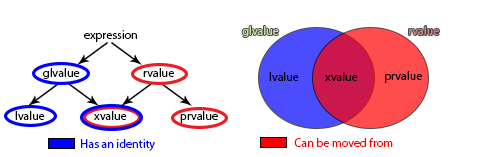
\includegraphics[scale=0.9]{value_categories.png}\\
	\subsection{Perfect forwarding}
	Пусть у нас имеется функция g, которая принимает какой-то аргумент и должна в чистом виде передать этот аргумент в функцию f. У нас есть три варианта передачи: по значению, по ссылке и по константной ссылке. При этом, если у функции f есть перегрузки по всем трем вариантам, встает вопрос, какой из этих вариантов реализовать в функции g. Кажется, что мы либо сделаем лишнее копирование, либо потеряем способность менять объект по ссылке, либо потеряем const. То есть, мы хотим при передаче аргумента через g в f сохранять не только значение, но и информацию, был ли он rvalue или lvalue, const или не const. Можно конечно написать несколько перегрузок, но в С++11 появилась возможность этого не делать. Для начала поговорим, как схлопываются ссылки. В С++ если к ссылке попытаться дописать еще один амперсанд, он схлопнется и даст просто ссылку. Это было сделано для того, чтобы частичная специализация шаблона, рассчитанная на получение ссылочного типа, могла работать, если в качестве типа передать ей уже ссылочный тип.
	\begin{minted}[tabsize=4, autogobble]{C++}
		template <typename T>
		void f(T&) {}
		
		void test() {
			int a;
			f<int&>(a);
			// T = int&
			// T& = int& & = int&
		}
	\end{minted}
	\textit{Замечание.} Просто так написать ссылку на ссылку не получится, это работает только с шаблонами.\\
	В С++11 схлопывание ссылок доопределили с учетом появившихся rvalue ссылок.
	\begin{minted}[tabsize=4, autogobble]{C++}
		// &   & ->  &
		// &  && ->  &
		// &&  & ->  &
		// && && -> &&
	\end{minted}
	Также доопределили дедукцию шаблонных параметров. С обычными шаблонами константность и ссылочность не дедусятся, но для rvalue ссылок это работает. Посмотрев на то, как работает дедукция с rvalue ссылками, вы поймете, зачем схлопывание определили именно так а не иначе. Это было сделано, чтобы использовать шаблоны с rvalue ссылками для той самой передачи с сохранением lvalue/rvalue и const.
	\begin{minted}[tabsize=4, autogobble]{C++}
		template <typename T>
		void qux(T&&) {}
		
		void test() {
			int a = 42;
			int const b = 43;
			
			qux(a);  // T -> int&
			qux(b);  // T -> int const&
			qux(42); // T -> int
		}
	\end{minted}
	Теперь мы наконец можем сделать perfect forwarding:
	\begin{minted}[tabsize=4, autogobble]{C++}
		void f(char&);
		void f(double);
		void f(std::string const&);
		void f(std::vector&&);
		
		template <typename T>
		void g(T&& arg) {
			f(static_cast<T&&>(arg));
		}
	\end{minted}
	Вместо статик каста можно использовать std::forward, а вот пример того, как он может быть реализован. Стоит заметить, однако, что нашему форварду нельзя забывать написать <T>, так как иначе тип выведется неправильно и всегда будет приводить к касту в rvalue, из-за чего произойдет мув и убьет наш объект. Библиотечный просто заставляет писать тип, и если забыть, ничего не скомпилируется.
	\begin{minted}[tabsize=4, autogobble]{C++}
		template <typename T>
		T&& forward(T& arg) {
			return static_cast<T&&>(arg);
		}
		
		template <typename T>
		void g(T&& arg) {
			f(forward<T>(arg));
		}
	\end{minted}
	\textit{Замечание}. В разделе про мув мы написали реализацию, отличную от таковой в стандартной библиотеке. Дело в том, что наша реализация может принимать только lvalue и кастить его к rvalue, но в стандартной библиотеке мув принимает что угодно, стирает ссылку и возвращает всегда rvalue.\\
	\textit{Замечание.} Т с двумя амперсандами в шаблоне называется универсальной ссылкой, так как принимает и rvalue, и lvalue.\\
	Есть прикольный способ запретить компилятору дедьюсить шаблон, то есть вычислять тип аргумента в случае если этот тип не указан в явном виде:
	\begin{minted}[tabsize=4, autogobble]{C++}
		template <typename T>
		struct no_deduce {
			using type = T;
		};
		
		template <typename T>
		void f(typename no_deduce<T>::type);
		
		void test() {
			f<int>(42); // ok
			f(42);      // compile error!!
		}
	\end{minted}
	Такая штука используется в библиотечном форварде, чтобы просто запретить вызывать его без указания типа в явном виде.\\
	Теперь можем написать реализацию make\textunderscore unique:
	\begin{minted}[tabsize=4, autogobble]{C++}
		template <typename T, typename... Args>
		std::unique_ptr<T> make_unique(Args&&... args) {
			return std::unique_ptr<T>(new T(std::forward<Args>(args)...));
		}
	\end{minted}
	\subsection{Decltype}
	Что если мы хотим сделать форвардинг в обратную сторону, то есть вернуть в g тот же тип, который возвращает f? Для этого придумали различные конструкции, одна из которых decltype. Это просто штучка, которая возвращает тип выражения (с учетом ссылочности конечно). У decltype есть вариация от имени:
	\begin{minted}[tabsize=4, autogobble]{C++}
		int a;
		
		struct foo {
			int b;
		};
		
		int& f();
		
		// decltype(2 + 2) -> int
		// decltype(a)     -> int
		// decltype(foo:b) -> int
		// decltype(f)     -> int&
	\end{minted}
	С decltype есть забавный момент. Если мы напишем внутри просто a, для него это будет именем, и тип выведется как у соответствующей переменной. Однако, если написать (a), это посчитается за выражение и тип будет ссылочный, так как есть переменная a и это выражение на нее ссылается.
	\begin{minted}[tabsize=4, autogobble]{C++}
		int a;
		
		decltype(a)   x; // int x
		decltype((a)) y; // int& y;
	\end{minted}
	Как же нам использовать decltype для форвардинга возвращаемого значения? Делается это весьма хитрым образом:
	\begin{minted}[tabsize=4, autogobble]{C++}
		template <typename T>
		T&& declval();
		
		template <typename T>
		decltype(f(declval<T>())) g(T&& arg) {
			return f(std::forward<T>(arg));
		}
	\end{minted}
	Было бы намного проще вместо лишней функции написать просто decltype от выражения в ретурне, но, увы, когда мы пишем тип возвращаемого значения, компилятор еще не видит аргументы, поэтому в С++11 появилась возможность писать возвращаемое значение в конце объявления функции.
	\begin{minted}[tabsize=4, autogobble]{C++}
		template <typename T>
		auto g(T&& arg) -> decltype(f(std::forward<T>(arg))) {
			return f(std::forward<T>(arg));
		}
	\end{minted}
	Трудно не заметить, что приходится дублировать выражение из ретурна, поэтому начиная с С++14 появился decltype(auto):
	\begin{minted}[tabsize=4, autogobble]{C++}
		template <typename T>
		decltype(auto) g(T&& arg) {
			return f(std::forward<T>(arg));
		}
	\end{minted}
	Стоит пару слов сказать про auto. В подавляющем большинстве случаев авто выводит тип так же, как шаблоны. В свою очередь decltype(auto) выводит тип выражения как если бы вместо авто подставили это выражение. Авто не сохраняет ссылки и консты, но decltype(auto) сохраняет.\\
	\textit{Замечание.} И у auto, и у шаблонов есть ситуация, когда выводится ссылочный тип. Это случается, когда в универсальную ссылку передают lvalue, тогда, чтобы при дописывании двух амперсандов он не превратился в обычный rvalue, к типу дописывают еще одну ссылку.
	\textit{Замечание.} Если функция имеет несколько return разного типа (например, в разных ветках if), auto и decltype(auto) не смогут вывести тип, придется написать явно, к чему приводить все эти возвращаемые значения.
	\par С perfect forwarding есть одна маленькая проблемка. Как мы знаем, ноль кастуется в нулевой указатель. Однако, perfect forwarding оказался не совсем perfect, поэтому он этот каст не смог протащить:
	\begin{minted}[tabsize=4, autogobble]{C++}
		void f(double const*);
		
		template <typename T>
		decltype(auto) g(T&& arg) {
			return f(std::forward<T>(arg));
		}
		
		int main() {
			f(0); // ok
			g(0); // T -> int
		}
	\end{minted}
	В С++11 эту проблему починили, создав специальное ключевое слово для нулевого указателя -- nullptr. Да, до С++11 его не было...\\
	Немного про временные объекты: допустим у нас есть поле класса, которое мы хотим вернуть и записать его по ссылке в локальную переменную. Что произойдет, когда временный объект умрет при переходе на следующую строчку? Ссылка начнет ссылаться на труп. Чтобы этого не происходило, существует правило: ссылка продлевает время жизни временного объекта до того момента, пока сама не откинется. С rvalue ссылками это тоже работает.
	\begin{minted}[tabsize=4, autogobble]{C++}
		struct person {
			public:
			std::string get_name() {
				return name;
			}
			private:
			std::string name;
		};
		
		void foo(person const& p) {
			std::string const& name = p.get_name();
		}
	\end{minted}
	Небольшое лирическое отступление: у мапы тип ключа на самом деле константный. Если этого не учесть, при итерировании будет лишнее копирование.
	\begin{minted}[tabsize=4, autogobble]{C++}
		void foo(std::map<std::string, int> const& m) {
			for (std::pair<std::string const, int> const& p : m) { // for (auto const& p : m) is better
				// ...
			}
		}
	\end{minted}
	Вообще, если вы хотите проитерироваться по контейнеру и просто посмотреть на элементы, то можно использовать константную ссылку, но если хотите менять их, используйте универсальную ссылку:
	\begin{minted}[tabsize=4, autogobble]{C++}
		std::vector<bool> v = {true, false, true};
		
		for (auto&& e : v) {
			e = !e;
		}
	\end{minted}
	\section{Intrusive контейнеры}
	Предположим, мы хотим завести LRU-кэш в виде мапы, которая может быстро обращаться к своим элементам не только по ключу, но и по времени последнего использования. Это значит, что она должна совмещать в себе мапу и двусвязный список. Вот пример узла такой структуры:
	\begin{minted}[tabsize=4, autogobble]{C++}
		struct node {
			Key key;
			Value value;
			
			// ordered by key (map)
			node* left;
			node* right;
			node* parent;
			
			// ordered by access time (list)
			node* prev;
			node* next;
		};
	\end{minted}
	Есть ли какой-то способ вынести общий код для таких двойных структур? Рассмотрим код юнита, который хранится в двух двусвязных списках -- all units и selected units:
	\begin{minted}[tabsize=4, autogobble]{C++}
		struct list_element {
			list_element* prev;
			list_element* next;
		};
		
		struct unit {
			list_element all_units_node;
			//...
			list_element selected_node;
			//...
		};
	\end{minted}
	К сожалению, привязка юнита к списку односторонняя, то есть как только мы попали в соответствующий юниту узел, дальше, передвигаясь по списку, мы будем получать только узлы списка, но не юниты. Юнит представляет собой два последовательно лежащих в памяти узла списка, из которых хотелось бы получить юнит целиком. \\
	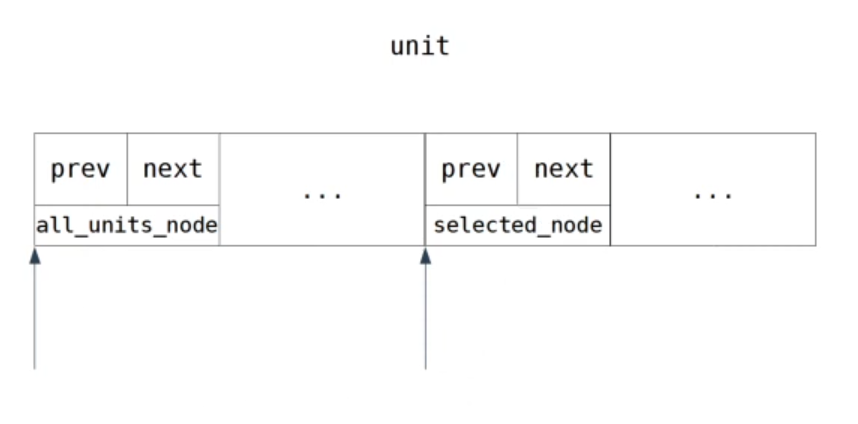
\includegraphics[scale=0.5]{unit.png}\\
	Здесь нам хочется как-то подвинуть указатель, чтобы собрать юнит из двух узлов списка. В С++ есть такой способ -- с помощью кастов, как если бы наш юнит наследовался от двух list element. Однако, мы не можем дважды отнаследоваться от list element, поэтому можно прибегнуть к помощи шаблонов, чтобы <<разделить>> структуру list element на две и отнаследоваться от них.
	\begin{minted}[tabsize=4, autogobble]{C++}
		template <typename Tag>
		struct list_element {
			list_element* prev;
			list_element* next;
		};
		
		struct all_units_tag;
		struct selected_tag;
		
		struct unit : list_element<all_units_tag>, list_element<selected_tag>
		{
			list_element all_units_node;
			//...
			list_element selected_node;
			//...
		};
		
		intrusive_list<unit, all_units_tag> all_units;
		intrusive_list<unit, selected_tag> selected_units;
	\end{minted}
	То, что сейчас было, называется intrusive контейнером.\\
	У нашей реализации с тэгом есть существенный минус: в функциях вроде erase, где нам плевать на тэг узла, приходится все равно помнить тэг, что приводит к генерации кода каждой функции столько раз, сколько у нас тэгов. Решение -- завести базовый класс и отнаследовать от него тэговые узлы, причем в erase использовать указатель на базовый класс:
	\begin{minted}[tabsize=4, autogobble]{C++}
		struct_list_element_base {
			list_element_base* prev;
			list_element_base* next;
		};
		
		template <typename Tag>
		struct list_element : list_element_base {};
		
		void erase(list_element_base* node) {
			node->prev->next = node->next;
			node->next->prev = node->prev;
			node->prev = nullptr;
			node->next = nullptr;
		}
	\end{minted}
	Это упрощенный пример кода, но в настоящей реализации мы бы хотели скрыть наш базовый класс, чтобы сторонний пользователь не мог сконвертить производный класс в базовый. Это делается с помощью приватного наследования:
	\begin{minted}[tabsize=4, autogobble]{C++}
		struct_list_element_base {
			list_element_base* prev;
			list_element_base* next;
		};
		
		template <typename Tag>
		struct list_element : private list_element_base {};
	\end{minted}
	\section{Shared Ptr}
	Shared pointer это умный указатель, то есть как и unique pointer он сам отвечает за удаление объекта, на который ссылается, но в отличие от unique умеет копироваться. Он хранит информацию о типе объекта и о количестве ссылок, которые на него ссылаются, причем это количество является общим для всех указателей на объект.\\
	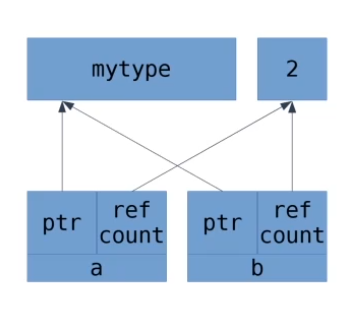
\includegraphics[scale=0.8]{shared.png}\\
	Shared pointer хранит общий счетчик ссылок как отдельный объект в памяти, что, наверно, не очень удобно, и было бы проще хранить этот счетчик внутри самого объекта, но shared ptr обязан ничего не требовать от объекта, на который ссылается, этим занимается intrusive ptr.\\
	Помимо счетчика ссылок shared ptr хранит информацию о deleter'e -- структуре, которая знает как удалять объект нужного типа. Спойлер: не всегда удаление объекта это operator delete, хотя дефолтный deleter делает именно это.\\
	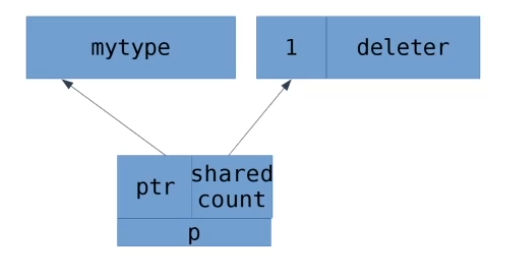
\includegraphics[scale=0.8]{deleter.png}\\
	Заметим, что в отличие от обычного объекта и unique ptr, shared ptr может пережить объект, который им пользуется. Это стоит брать в расчет при использовании shared ptr, так как ссылаться на объект, созданный другим объектом, имеет смысл только в течение жизни того объекта. Из-за того что shared продлевает время жизни объекта, на который ссылается, можно получить утечку, если слишком долго держать объект в памяти.\\
	Рассмотрим пример, когда класс vehicle ссылается на объекты wheel с помощью shared ptr. 
	\begin{minted}[tabsize=4, autogobble]{C++}
		struct vehicle {
			std::array<std::shared_ptr<wheel>, 4> wheels;
		};
	\end{minted}
	Мы можем хотеть, чтобы был именно shared ptr, но при этом чтобы время жизни vehicle было не меньше чем у wheel. Для этого придумали aliasing конструктор. Этот специальный конструктор помимо указателя на область памяти принимает также объект, с которым будет общее число ссылок. Так же теперь помимо счетчика ссылок будет дополнительно храниться указатель на этот объект, чтобы он всегда был удален последним. \\
	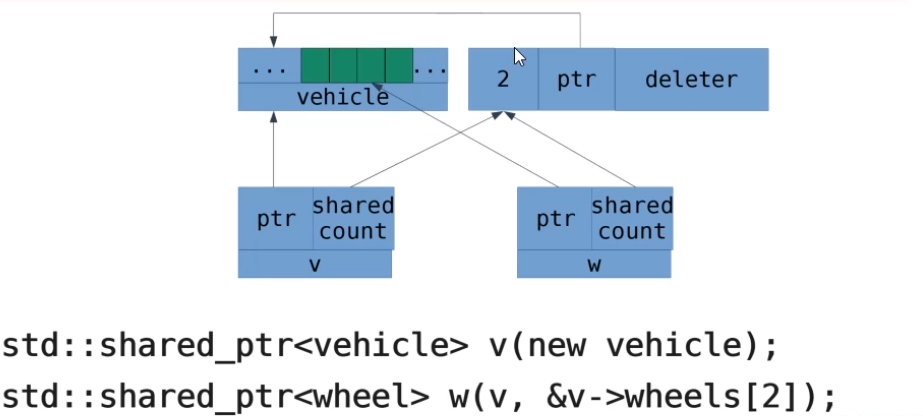
\includegraphics[scale=0.5]{aliasing_ctor.png}\\
	В обычном конструкторе shared ptr мы сначала одной аллокацией создаем объект, а потом передаем его как аргумент конструктора и делаем вторую аллокацию уже для дополнительной информации shared ptr (число ссылок и т.д.). Можно объединить эти две аллокации в одну с помощью make shared (так же как make unique). При этом в make shared нельзя передать deleter, потому что shared ptr сам создает объект в этом случае и сам же знает как его удалять.\\\par
	Парой к shared ptr является объект weak ptr, который может продолжать жить при удаленном объекте. Его нелья разыменовать, а служит он только чтобы проверять, не удалился ли объект. Это нужно для многопоточности, где чужой поток может удалить общий объект. С наличием weak ptr добавляется поле, хранящее число слабых ссылок +1, если есть хотя бы одна сильная ссылка (weak ptr'ы не учитываются при подсчете сильных ссылок).
	\\ \textit{Замечание}. Пока жив weak ptr, жив и control block (счетчик ссылок), так как он нужен для проверки, не удалился ли объект. В случае, если был использован make shared, то есть объект и control block были созданы одной аллокацией, на объекте вызовется деструктор при удалении, но память из под него не будет освобождена до смерти weak ptr.\\
	\textit{Замечание}. Если при инициализации shared ptr не удалось создать control block, на уже созданном объекте вызывается deleter.\\
	\par Предположим, что мы храним в мапе weak ptr на виджет, к которому идет обращение по shared ptr. Weak ptr нам здесь нужен, чтобы не мешать объекту удаляться, так как мапа используется только для поиска. Однако, хочется сделать так, чтобы при удалении виджета запись в мапе тоже сама удалялась, дабы не держать в памяти control block. Выход прост: изменить deleter виджета, чтобы он удалял запись из мапы weak ptr'ов.\\
	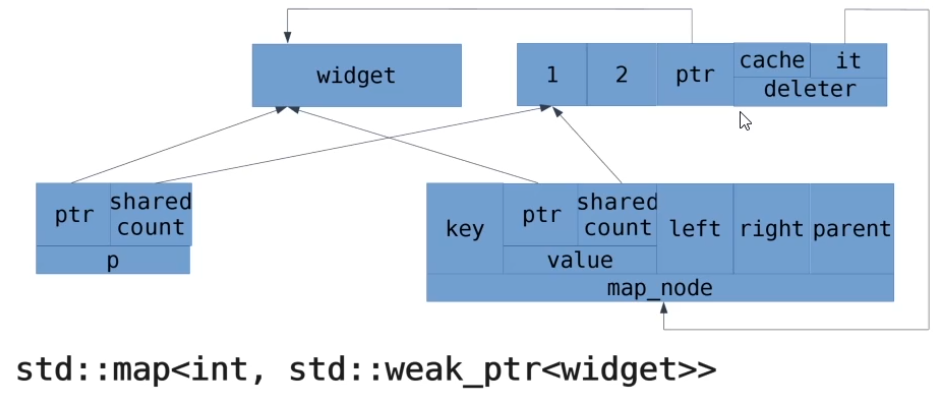
\includegraphics[scale=0.5]{weak_map.png}\\
	Все синие кусочки на картинке имеют одинаковое время жизни, поэтому хотелось бы некоторые из них объединить. Например, виджет и control block с помощью make shared. Но make shared не позволяет иметь deleter, поэтому мы напишем класс-обертку с деструктором, который делает то, что делал бы deleter. При этом у нас будет shared ptr на обертку, а мы хотим на виджет, поэтому воспользуемся aliasing ctor.
	\\\par Стоит заметить, что у shared ptr есть конструктор от обычного указателя, но каждый вызов этого конструктора приводит к созданию нового control block. Хуже лишнего выделения памяти здесь только попытка повторного удаления, когда в одном control block число ссылок уже давно 0 и объект был удален, а во втором только опустилось до нуля.
	\begin{minted}[tabsize=4, autogobble]{C++}
		void bad() {
			int* p = new int(42);
			
			std::shared_ptr<int> sp1(p); // new control block
			std::shared_ptr<int> sp2(p); // new control block
		}
	\end{minted}
	Такая же ошибка может возникнуть, когда мы хотим вернуть shared ptr на this. Если написать конструктор от this, будет каждый раз создаваться новый control block. Чтобы избежать этого, надо отнаследовать наш класс от класса enable shared from this.
	\begin{minted}[tabsize=4, autogobble]{C++}
		class good : public std::enable_shared_from_this<good> {
			std::shared_ptr<good> foo() {
				return shared_from_this();
			}
		};
	\end{minted}
	Public наследование здесь написано специально, так как по умолчанию class наследуется приватно, то есть shared ptr как и остальные классы не будет знать об этом наследовании и shared from this не сработает.
	\\\textit{Замечание}. Shared from this не работает в конструкторах.
	\par Внутри класс enable shared from this устроен очень просто: он хранит mutable weak ptr, от которого создаются shared ptr, хранящие указатель на наследника. Конструктор shared ptr умеет распознавать, что объект наследуется от enable shared from this, и в этом случае записывает в weak ptr указатель на объект, на который ссылается.
	\section{Работа с функциями}
	\subsection{Лямбды}
	В старых версиях C++ пользоваться функциями как объектами можно было только создав структуру, у которой есть оператор круглые скобки, в силу статического полиморфизма C++. Понятно, что это достаточно неудобно, особенно если это одноразовая функция, такая как компаратор. Теперь в языке появись анонимные функции или лямбды.
	\begin{minted}[tabsize=4, autogobble]{C++}
		struct comp {
			bool operator()(int a, int b) const {
				return a % 7 < b % 7;
			}
		};
		
		void foo(std::vector<int>& v) {
			std::ranges::sort(v, comp());
			std::ranges::sort(v, [](int a, int b) { return a % 7 < b % 7; });
		}
	\end{minted}
	Как это работает? Компилятор генерирует код структуры с оператором круглые скобки, причем возвращаемое значение такого оператора определяется автоматически, но его можно указать явно, если вывод компилятора не подходит.
	\begin{minted}[tabsize=4, autogobble]{C++}
		auto a = []{};
		auto b = [](int a, int b){ return a + b; };
		auto c = [](int a, int b) -> int { return a + b; };
	\end{minted}
	Зачем в примере выше пишутся эти пустые квадратные скобки? На самом деле, в них можно написать, что лямбда захватывает при генерации структуры. Пусть мы хотим создать структуру-компаратор, которая сравнивает но по остатку от деления на 7, а по остатку от деления на n. Мы бы создали у нее конструктор, в который передали бы n. Лямбды тоже позволяют это сделать.
	\begin{minted}[tabsize=4, autogobble]{C++}
		struct comp {
			comp(int n) : n(n) {}
			
			bool operator()(int a, int b) const {
				return a % n < b % n;
			}
			
			private:
			int n;
		};
		
		void foo(std::vector<int>& v, int n) {
			std::ranges::sort(v, comp(n));
			std::ranges::sort(v, [n](int a, int b) { return a % n < b % n; });
		}
	\end{minted}
	Переменные можно захватывать по ссылке и по значению. Причем можно сказать <<захвати все используемые в лямбде переменные по значению кроме некоторых>> и аналогично по ссылке.
	\begin{minted}[tabsize=4, autogobble]{C++}
		auto e = [x, &y, z](){}; // x and z by value, y by reference
		auto f = [=, &y](){};    // everything by value except y
		auto g = [&, x, z](){};  // everything by reference except x and z
	\end{minted}
	В C++11 можно было захватывать this, а начиная с C++17 даже можно захватить копию this:
	\begin{minted}[tabsize=4, autogobble]{C++}
		// C++11
		[this](){};
		[=](){};
		[&](){};
		
		//C++17
		[*this](){}; // by copy
		
		/*
		=       x      *this
		&      &x       this
		*/
	\end{minted}
	Мы можем хотеть помувать захваченный объект, для этого есть специальная форма именованного захвата:
	\begin{minted}[tabsize=4, autogobble]{C++}
		template <typename F>
		void bar(F);
		
		void foo(std::string str) {
			bar([str = std::move(str)]{});
		}
	\end{minted}
	Стоит обратить внимание, что по дефолту оператор круглые скобки, который генерируется для лямбд, имеет модификатор const, а значит все захваченные переменные являются константными. Это поведение можно изменить с помощью модификатора mutable:
	\begin{minted}[tabsize=4, autogobble]{C++}
		size_t x = 0;
		[&x](int a) mutable {
			++x;
			return x;
		};
	\end{minted}
	Еще немного примеров синтаксиса лямбд:
	\begin{minted}[tabsize=4, autogobble]{C++}
		auto a = []<typename T>(T x){ return x; };
		auto b = [](auto x){ return x; }
		auto c = [](int a) static { return a + 42; }; // C++23 only
	\end{minted}
	Обратите внимание, что в шаблонной лямбде шаблонный именно оператор круглые скобки, а не сама структура. Еще один момент -- лямбды могут конвертиться в указатель на функцию, но только те, кто не захватывает переменные. При этом глобальные и статические переменные можно не захватывать, они и так доступны. 
	\subsection{std::function}
	Представьте, что вы хотите работать с переменной, значение которой функция (у нас не хаскель, но допустим). Какой тип нужно написать при объявлении переменной, чтобы потом, например, положить туда значение внутри одной из веток ифа? Некоторые могут сказать, что можно написать auto, но auto не сможет вывести тип, если значение не указано при объявлении. Может быть, раз мы используем иф, нужно переписать его как тернарник и проинициализировать переменную сразу при объявлении? Но и в этом случае auto не будет работать, так как ветки тернарника имеют разные типы (каждая лямбда это отдельный тип). На помощь приходит std::function. Этот волшебный тип из стандартной библиотеки принимает как шаблон типы аргументов и возвращаемое значение, и дальше в переменную такого типа можно присвоить любую функцию с такими же типами. Например:
	\begin{minted}[tabsize=4, autogobble]{C++}
		struct greater {
			bool operator()(int a, int b) {
				return a > b;
			}
		};
		
		struct less {
			bool operator()(int a, int b) {
				return a < b;
			}
		};
		
		void test(std::vector& v, bool flag) {
			std::function<bool (int, int)> comp;
			if (flag)
				comp = less(); // this is a ctor, not function call :D
			else
				comp = greater();
			// comp = [](int a, int b){ return false; }
			std::ranges::sort(v, comp);
		}
	\end{minted}
	Как вы наверно уже догадались, внешний вид шаблонного параметра std::function означает, что туда передается функция с определенным типом аргументов и возвращаемым значением. Вот как это выглядит непосредственно внутри std::function:
	\begin{minted}[tabsize=4, autogobble]{C++}
		template <typename Sig>
		struct function;
		
		template <typename R, typename... Args>
		struct function<R (Args...)> {};
	\end{minted}
	\subsection{Type erasure}
	Пусть мы хотим написать такой класс function\textunderscore int, для которого работает следующий код:
	\begin{minted}[tabsize=4, autogobble]{C++}
		struct function_int {
			//...
		};
		
		struct foo {
			void operator()(int) {
				std::cout << "foo\n";
			}
		};
		
		struct bar {
			void operator()(int) {
				std::cout << "bar\n";
			}
		};
		
		int main() {
			function_int f = foo();
			f = bar();
		}
	\end{minted}
	У нашего класса должен быть конструктор, принимающий функцию, которая потом сохраняется как поле класса. Поскольку все функции это разные типы, конструктор должен быть шаблонным, однако тогда этот шаблон не распространяется на приватные поля.
	\begin{minted}[tabsize=4, autogobble]{C++}
		// doesn't compile
		struct function_int {
			template <typename F>
			function_int(F func) : func(func) {}
			
			private:
			F func; // who the f is F? compiler doesn't see outside the template
		};
	\end{minted}
	Кто-то может посоветовать распространить шаблон на весь класс, но \sout{это было бы слишком легко} теряется наша фишка сохранения разных функций в одной переменной (при объявлении придется в явном виде написать класс функции, который мы положим, и поменять его уже будет нельзя).\\
	Есть решение с динамической аллокацией, автору конспекта оно ужасно не нравится, так как это полное издевательство над системой типов (речь конечно же про void*). К тому же, как и ожидается от плохого решения, с полученной функцией не то что работать нельзя, но даже удалить нормально не получится, так как для удаления нужно знать исходный тип.
	\begin{minted}[tabsize=4, autogobble]{C++}
		struct function_int {
			template <typename F>
			function_int(F func) 
			: func(new F(std::move(func))) 
			{}
			
			private:
			void* func;
		};
	\end{minted}
	В итоге мы упираемся в проблему: хочется как-то запомнить тип нашей функции, чтобы пользоваться им за пределами шаблона. Можно сделать хитрый трюк: создать еще одну шаблонную структурку, которая будет кастовать объект в нужный тип и удалять.
	\begin{minted}[tabsize=4, autogobble]{C++}
		template <typename F>
		void destroy_impl(void* ptr) {
			delete static_cast<F*>(ptr);
		}
		
		struct function_int {
			using destroy_t = void (*)(void*);
			
			template <typename F>
			function_int(F func) 
			: func(new F(std::move(func))) 
			, destroy(&destroy_impl<F>)
			{}
			
			~function_int() {
				destroy(func);
			}
			
			private:
			void* func;
			destroy_t destroy;
		};
	\end{minted}
	Соответственно, такую структурку можно сделать не только для деструктора, но и для копирования и вызова. При этом можно создавать пустой function, для которого указатель на функцию nullptr, структурки копирования и удаления ничего не делают, а структурка вызова бросает bad function call. Стоит также не забыть, что при присваивании необходимо присвоить структурки тоже.\\
	\par Я понимаю тех, кому как и мне не нравятся махинации с бедной слабой системой типов, поэтому вот решение получше: заводим какой-то класс-обертку, который инстанцируется шаблоном целиком и хранит в себе нашу функцию. Обертка наследуется от базового класса без шаблона, у которого деструктор, копирование и вызов виртуальные, вот и всё.
	\begin{minted}[tabsize=4, autogobble]{C++}
		struct concept_ {
			virtual ~concept() {}
			virtual std::unique_ptr<concept_> copy() const = 0;
			virtual void call(int arg) const = 0;
		};
		
		template <typename F>
		struct model : concept_ {
			explicit model(F func) : func(std::move(func)) {}
			
			std::unique_ptr<concept_> copy() const override {
				return std::make_unique<model<F>>(*this);
			}
			
			void call(int arg) const override {
				return func(arg);
			}
			
			private:
			F func;
		};
		
		struct function_int {
			template <typename F>
			function_int(F func) 
			: func(new model<F>(std::move(func)))
			{}
			
			function_int(function_int const& other) 
			: func(other.func->copy())
			{}
			
			function_int& operator=(function_int const& other) {
				func = other.func->copy();
				return *this;
			}
			
			void operator()(int arg) const {
				return func->call(arg);
			}
			
			private:
			std::unique_ptr<concept_> func;
		}
	\end{minted}
	Возможно вы задавались вопросом: почему бы не сделать итераторы полиморфными, ведь нам нет никакой разницы, итерируемся мы по узлам списка или сета. Во-первых, динамический полиморфизм подразумевает работу с указателями, а не с самими объектами, а это лишние аллокации. Во-вторых, полиморфное поведение итераторов нужно нам не так часто, а платить за него пришлось бы постоянно. Поэтому в стандартной библиотеке нет таких итераторов, но это не значит что их нет вообще. Можно представить себе итератор, который как и function\textunderscore int может хранить любой итератор на int. Такие итераторы называются any итераторы. Но что если мы не ограничимся итераторами и сделаем тип, в который можно положить все что умеет копироваться и создаваться? Такой тип в стандартной библиотеке есть и называется any. Каст из any в тип, который там хранится, называется any\textunderscore cast. Такой подход, когда мы объединяем несколько типов в один с помощью полиморфизма называется type erasure.
	\par На самом деле можно заметить, что type erasure делает что-то похожее на наследование, но здесь есть несколько ключевых отличий. Во-первых, наследование интрузивное, то есть в самом классе нужно писать что он наследуется, а type erasure может взять два абсолютно разных класса и сказать, что один из них реализует интерфейс другого. Это можно сделать с помощью специального класса adapter, для которого указать, что он реализует интерфейс, и просто внутри перевызывать методы. Во-вторых, при наследовании пользователю приходится снаружи работать с указателями, чтобы иметь доступ к динамическому типу, а в erasure наличие указателей -- деталь реализации, скрытая в самой структуре.
	\subsection{Сигналы}
	На самом деле std::function это частный случай сигналов (signal, listener, observer). Представим, что мы хотим хранить вектор функций, каждая из которых соответствует определенному событию, например изменению текста в ячейке. Это и есть сигнал. Для лучшего понимания рассмотрим его примитивную реализацию:
	\begin{minted}[tabsize=4, autogobble]{C++}
		struct signal {
			using slot_t = std::function<void ()>;
			
			void connect(slot_t slot) {
				slots.push_back(std::move(slot));
			}
			
			void operator()() const {
				for (slot_t const& slot : slots) {
					slot();
				}
			}
			
			private:
			std::vector<slot_t> slots;
		};
	\end{minted}
	У нас в реализации есть функция connect, логично захотеть сделать функцию disconnect наподобие такой:
	\begin{minted}[tabsize=4, autogobble]{C++}
		void disconnect(slot_t slot) {
			auto it = std::ranges::find(slots, slot);
			slots.erase(it);
		}
	\end{minted}
	Упс, это не компилируется. Почему? Find внутри себя использует сравнение на равенство, а функции не умеют сравниваться. Да и в целом, допустим мы положили в слот лямбду, а что мы передадим, если захотим удалить ее?
	\par Можно придумать следующее решение: пусть connect возвращает некий объект типа connection, а disconnect по этому объекту сможет удалить нужную функцию из вектора. Но тут возникает проблема: пусть мы храним итератор или индекс на позицию в векторе, тогда при удалении элемента где-то в середине все connection'ы справа инвалидируются. Есть два решения: хранить вместо вектора мапу из пары ID-function или хранить вместо вектора std::list. В первом случае оператор круглые скобки выглядит примерно так:
	\begin{minted}[tabsize=4, autogobble]{C++}
		void signal::operator()() const {
			for (auto const& p : id_to_slot) {
				p.second();
			}
		}
	\end{minted}
	Только вот этот код приводит к UB, как и аналогичный код с std::list. Рассмотрим случай, когда функция внутри сигнала дисконнектит сама себя. Тогда внутри оператора круглые скобки, внутри цикла вызовется функция, которая удалит элемент из контейнера, и после этого цикл, попытавшись перейти к следующему элементу, просто умрет, потому что текущий элемент удален. Проблема здесь именно в инкременте итератора, которое не выполнится на невалидном итераторе. Можно конечно руками инкрементить итератор, а потом уже удалять элемент, но в общем случае это не помжет: что если функция дисконнектит не себя, а следующую за ней? Есть решение сделать копию контейнера и вызываться на нем:
	\begin{minted}[tabsize=4, autogobble]{C++}
		void signal::operator()() const {
			std::list<slot_t> copy = slots;
			for (auto const& p : copy()) {
				p();
			}
		}
	\end{minted}
	Тут снова есть проблема, например, если дисконнект происходит в деструкторе какой-то структуры:
	\begin{minted}[tabsize=4, autogobble]{C++}
		struct mytype {
			mytype(signal& timeout_signal)
			: timeout_conn(timeout_signal.connect([this]() { // do smth }))
			{}
			
			~mytype() {
				timeout_conn.disconnect();
			}
			
			private:
			signal::connection timeout_conn;
		}; 
	\end{minted}
	То что вызван дисконнект в нашем случае не будет означать моментальное удаление из списка, так как функция все еще останется внутри копии списка, а учитывая, что функция захватывает this и потенциально использует данные уже удаленного объекта, будет очень плохо.
	\par Наконец, есть еще одно решение: не удалять в прямом смысле, а присваивать в слот пустую функцию и в конце подчищать их.
	\begin{minted}[tabsize=4, autogobble]{C++}
		private:
		mutable std::list<slot_t> slots; // slots can be changed inside const signal
		
		public:
		void signal::connection::disconnect() {
			// sig->slots.erase(it);
			*it = slot_t();
		}
		
		void signal::operator()() const {
			for (slot_t const& slot : slots) {
				if (slot)
					slot();
			}
			
			for (auto i = slots.begin(); i != slots.end(); ++i) {
				if (*i)
					++i;
				else
					i = slots.erase(i);
			}
		}
	\end{minted}
	\textit{Замечание}. Mutable означает, что это поле может меняться даже в константном объекте.\\
	Тут всё еще есть проблема, если слот рекурсивно вызывает сам сигнал. Чтобы ее решить, давайте просто запоминать, правда ли мы внутри вызова самого сигнала:
	\begin{minted}[tabsize=4, autogobble]{C++}
		void signal::connection::disconnect() {
			if (sig->inside_emit) {
				*it = slot_t();
			} else {
				sig->slots.erase(it);
			}
		}
		
		void signal::operator()() const {
			bool old_inside_emit = inside_emit;
			inside_emit = true;
			
			try {
				for (slot_t const& slot : slots) {
					if (slot)
						slot();
				}   
			} catch (...) {
				inside_emit = old_inside_emit;
				if (!old_inside_emit)
					prune_empty_slots();
				throw;
			}
			
			inside_emit = old_inside_emit;
			if (!old_inside_emit) {
				prube_empty_slots();
			}
		}
		
		void prune_empty_slots() const {
			for (auto i = slots.begin(); i != slots.end(); ++i) {
				if (*i)
					++i;
				else
					i = slots.erase(i);
			}
		}
	\end{minted}
	Но что делать, если какой-то из слотов внутри своего вызова убил сигнал? Есть довольно прямолинейный способ решения этой проблемы: нужно просто сделать время жизни всех слотов равное времени жизни сигнала с помощью shared ptr. Еще один вариант -- завести указатель destroyed\textunderscore ptr, который будет равен nullptr или true, и очень аккуратно с его помощью сообщать всем вызовам, что надо прекращать работать с этим сигналом. Вообще, нюансов работы с сигналами очень много, далеко не все библиотеки гарантируют корректную работу во всех из вышеперечисленных случаев, да и не всегда это требуется. Вполне возможно, что вам хватит сделать ассерт внутри деструктора сигнала, что деструктор не был вызван слотом.
	\section{Optional и Variant}
	\subsection{Optional}
	Представим класс, который считает некое значение и кэширует его в свой мембер. При этом к этому мемберу можно обращаться только в том случае, когда в нем лежит актуальное значение. Для этого заведем флаг is\textunderscore initialized. Эту пару из значения и флага в стандартной библиотеке выделяют в класс optional. Optional конвертится в bool и разыменовывается по звездочке.
	\par Давайте подумаем, как можно реализовать optional (это будет на практике, хехе). Можем ли мы хранить значение T просто полем класса? Кажется нет, потому что дефолтный конструктор optional в любом случае будет пытаться его инициализировать, а мы не хотим требовать от нашего типа наличие дефолтного конструктора, да и суть optional как раз в хранении неинициализированных переменных. Что же мы будем делать? \\А) Просто запретим для optional дефолтный конструктор. \\B) Будем хранить union. \\C) Будем хранить массив типа std::byte размера sizeof(T).
	\par Вариант А это очевидно не то что мы хотим. У варианта C есть проблемы с выравниванием, так как тип Т может требовать другое выравнивание, чем выравнивание массива чаров такого же размера. Здесь есть решение: использовать aligned storage, ну либо написать alignas.\\
	\textbf{Замечание.} Aligned storage был помечен deprecated в C++23, но внутри он по сути просто является выровненным массивом байтов.\\р
	\begin{minted}[tabsize=4, autogobble]{C++}
		template <typename T>
		struct optional {
			private:
			bool is_initialized;
			std::aligned_storage_t<sizeof(T), alignof(T)> storage;
			// alignas(alignof(T)) std::byte storage[sizeof(T)];
		};
	\end{minted}
	Что насчет union, в C++03 можно было создавать union'ы только от структур с тривиальными конструкторами и деструкторами. В C++11 это требование ослабили, но union не может самостоятельно инициализировать свои поля, поэтому для нашего класса optional нужно будет явно написать конструктор и деструктор, которые правильно инициализируют содержимое union.
	\begin{minted}[tabsize=4, autogobble]{C++}
		template <typename T>
		struct optional {
			optional() {}
			~optional() {}
			private:
			bool is_initialized;
			union {
				T value;
			};
		};
	\end{minted}
	Давайте рассмотрим реализацию optional с aligned storage (с union будет аналогичная реализация):
	\begin{minted}[tabsize=4, autogobble]{C++}
		template <typename T>
		struct optional {
			optional() : is_initialized(false) {}
			
			optional(T value) : is_initialized(true) {
				new (&storage) T(std::move(value));
			}
			
			optional(optional const& other)
			: is_initialized(other.is_initialized)
			{
				if (is_initialized)
					new (&storage) T(reinterpret_cast<T const&>(other.storage));
			}
			
			optional(optional&& other)
			: is_initialized(other.is_initialized)
			{
				if (is_initialized) {
					new (&storage) T(
						std::move(reinterpret_cast<T&>(other.storage))
					);
				}
			}
			
			~optional() {
				if (is_initialized)
					reinterpret_cast<T&>(storage).~T();
			}
			
			explicit operator bool() const {
				return is_initialized;
			}
			
			T& const operator*() const {
				assert(is_initialized);
				return reinterpret_cast<T const&>(storage);
			}
			
			T& operator*() {
				assert(is_initialized);
				return reinterpret_cast<T&>(storage);
			}
			
			private:
			bool is_initialized;
			std::aligned_storage_t<sizeof(T), alignof(T)> storage;
		};
	\end{minted}
	У optional из стандартной библиотеки есть две крутые функции: конструктор с маркером std::in\textunderscore place и функция emplace. Обе нужны чтобы вместо создания объекта снаружи и последующего мува сразу создавать объект внутри optional (аналогично функции make\textunderscore unique у unique ptr). Обратите внимание, что emplace не дает строгую гарантию, а дает базовую, потому что, в отличие от присваивания готового объекта, чтобы сконструировать объект на конкретном участке памяти (storage), предыдущий объект придется безвозвратно удалить.
	\par Еще несколько приколов optiona'a: их можно сравнивать, причем пустой optional всегда меньше всего остального. Как и nullptr у указателя, у optional есть универсальный пустой тип nullopt. Как вы уже заметили, unique ptr является альтернативой optional'у, который иногда имеет смысл использовать вместо него, например если тип non-movable или нужно, чтобы он всегда лежал по одному адресу. Так же для маленьких объектов лучше использовать optional, потому что он не делает динамические аллокации, а для больших unique ptr, особенно если объект часто пустует, потому что unique ptr не резервирует память для пустых объектов. Также стоит понимать, что массив optional'ов из-за выравнивания хранить дороже, чем массив типа T + массив типа bool.
	\subsection{Noexcept}
	Если посмотреть на наш код в компиляторе, можно заметить предупреждение, что move конструктор должен быть noexcept. Почему это так? Одно из использований мува -- реаллокация вектора, то есть перенос его в другую область памяти. Это нужно во многих ситуациях, например при расширении вектора во время push back. Push back дает строгую гарантию, то есть исходный объект никак не должен быть испорчен, однако, если мы делаем реаллокацию не копированиями, а мувами, бросающий move может поставить нас в неприятное положение, когда элементы до текущего уже перенесены и к ним больше нельзя обращаться в исходной области памяти, а элементы начиная с текущего всё ещё лежат в старом месте, и с этим ничего сделать нельзя, потому что и старое, и новое хранилище в неполном состоянии. Поэтому было принято соглашение: вектор может использовать move, но только в том случае, если move не бросает. В языке есть функция noexcept (не путать с модификатором), которая позволяет проверить, является ли вычисление выражения noexcept:
	\begin{minted}[tabsize=4, autogobble]{C++}
		void foo() noexcept {}
		
		const bool is_noexcept = noexcept(foo());
	\end{minted}
	Напомним, что у модификатора noexcept есть специальный синтаксис, который позволяет задать условие, при котором функция noexcept. Зачем это нужно? А для шаблонов. Если у типа T небросающий мув, то и мувающий конструктор у optional<T> будет noexcept.
	\begin{minted}[tabsize=4, autogobble]{C++}
		optional(optional&& other) 
		noexcept(std::is_nothrow_move_constructible_v<T>)
		: is_initialized(other.is_initialized)
		{
			if (is_initialized)
				new (&storage) T(std::move(reinterpret_cast<T&>(other.storage)));
		}
	\end{minted}
	\textit{Замечание}. Можно написать noexcept от noexcept'а, где внутренний noexcept будет возвращать какое-то булево значение, которое будет определять внешний noexcept.
	\\ С присваиванием будет похитрее, потому что здесь у нас есть четыре случая, так как наш объект и другой объект могут быть как проинициализированы, так и нет.
	\begin{minted}[tabsize=4, autogobble]{C++}
		optional& operator=(optional&& other) 
		noexcept(std::is_nothrow_constructible_v<T> &&
		std::is_nothrow_move_assignable_v<T>)
		{
			if (is_initialized) {
				if (other.is_initialized)
					storage = std::move(other.storage);
				else {
					is_initialized = false;
					storage.~T();
				}
			} else {
				if (other.is_initialized)
					new (&storage) T(std::move(other.storage));
				is_initialized = true;
			}
		}
		
		return *this;
	}
\end{minted}
\subsection{Соблюдение трейтов}
Еще одно отличие optional стандартной библиотеки от нашего, помимо крутых noexcept -- SFINAE-friendliness. Что это такое? Пусть тип A конвертится в тип B, тогда optional от A должен конвертиться в optional от B. Если просто написать optional'у шаблонный конструктор от другого optional'а, получится так, что с точки зрения SFINAE снаружи все optional'ы конвертятся во все, даже если на самом деле этот шаблонный конструктор не будет работать для всех подряд типов.
\begin{minted}[tabsize=4, autogobble]{C++}
	template <typename T>
	struct optional {
		template <typename U>
		optional(optional<U> const&);
	};
	
	struct a {};
	struct b {};
	
	// !std::is_convertible_v<a, b>
	// !std::is_convertible_v<std::optional<a>, std::optional<b>>
	// std::is_convertible_v<optional<a>, optional<b>> wtf???
\end{minted}
Хочется, чтобы эта информация о конверсиях, копируемости и т.д. проникала в сам optional. Это не так-то просто сделать. А как именно это сделать -- вы узнаете на практике :)
\\\par Еще один момент, про который надо поговорить -- тривиальность копирования. Как мы знаем, при отсутствии конструктора копирования он генерируется компилятором. Но не все так просто. Если тип состоит из простейших типов вроде интов, никакой конструктор генерироваться не будет, а в местах, где он должен вызываться, просто сделается что-то вроде memcpy. Такой тип называется тривиально копируемым. При этом, если в явном виде написать конструктор копирования, в котором просто сделать то, что по идее делает этот конструктор по дефолту, то есть вызвать коирование у всех полей, свойство тривиальности копирования потеряется как раз из-за этой штуки с memcpy.
\begin{minted}[tabsize=4, autogobble]{C++}
	// trivially copyable
	struct a {
		int x;
		int y;
	};
	
	// non-trivially copyable
	struct b {
		b(const b& other)
		: x(other.x)
		, y(other.y)
		{}
		
		int x;
		int y;
	};
\end{minted}
Свойство тривиальности копирования, как и остальные свойства тривиальности, определяются рекурсивно: у класса не должно быть явного конструктора, все его поля должны обладать свойством тривиальности и все его базы должны обладать свойством тривиальности. Но почему нам вообще важна эта тривиальность? Есть три причины. Первая -- некоторые шаблонные классы просто требуют от типа тривиальность копирования, например std::atomic. Вторая -- оптимизации стандартной библиотеки, например вектор от тривиально копируемого типа может сделать memcpy вместо вызова обычного конструктора копирования. Третья -- зависимость ABI от тривиальности. Можно убедиться с помощью godbolt, что отсутствие тривиальности увеличивает размер ассемблерного кода в разы. По этой же причине кстати unique ptr не является zero-overhead абстракцией. На этот случай есть [[clang::trivial\textunderscore abi]], но он не входит в стандарт.\\
\textit{Замечание}. Trivially default constructible является подмножеством nothrow default constructible, который является подмножеством default constructible, который является подмножеством всех типов.\\
\textit{Замечание}. Optional помимо самой конверсии также сохраняет свойство explicit/implicit конверсии.
\subsection{Constexpr}
\par Рассмотрим код, который приводит к ошибке компиляции:
\begin{minted}[tabsize=4, autogobble]{C++}
	template <typename T>
	T const& max(T const& a, T const& b) {
		return a < b ? b : a;
	}
	
	template <typename A, typename B>
	struct either
	{
		size_t which;
		std::aligned_storage_t<max(sizeof(A), sizeof(B)),
							   std::lcm(sizeof(A), sizeof(B))> storage;
	};
	
	template struct either<int, float>;
\end{minted}
Ошибка компиляции здесь будет по той причине, что шаблонный параметр у aligned storage должен быть константой, известной на этапе компиляции. Да, функция max не делает ничего, что нельзя посчитать на этапе компиляции, но компилятор об этом не знает, в теории она может внутри себя обращаться к потоку ввода/вывода, например. В C++03 это обходили с помощью static const мемберов.
\begin{minted}[tabsize=4, autogobble]{C++}
	template <typename T, T a, T b>
	struct max {
		static T const value = a < b ? b : a;
	};
	
	template <typename A, typename B>
	struct either
	{
		size_t which;
		std::aligned_storage_t<max<std::size_t, sizeof(A), sizeof(B))>::value,
							       std::lcm(sizeof(A), sizeof(B))> storage;
	};
	
	template struct either<int, float>;
\end{minted}
Этот способ решения совсем не крутой, потому что это дублирование кода между обычной функцией max, которая работает в рантайме, и compile-time метафункцией (она так называется потому что для нас это функция, но с точки зрения языка это класс). Помимо шаблонных параметров compile-time вычисления интересуют нас в глобальных переменных. Там действует такое правило: если глобальная переменная инициализируется выражением, значение которого может подсчитать компилятор, он его подсчитает и сохранит, в противном случае сгенерирует код, который при запуске программы будет инициализировать переменную. Здесь мы тоже хотим сделать так, чтобы глобальные переменные вычислялись в compile-time, иначе они будут тормозить запуск программы.
\par Все это подводит нас к языковой конструкции constexpr. Constexpr бывает двух типов: constexpr на функции говорит, что эту функцию можно выполнить на этапе компиляции, например для вычисления шаблонных параметров, а constexpr на переменной говорит, что значение переменной обязательно будет посчитано во время компиляции, а не при запуске программы. Обратите внимание, что если мы инициализируем constexpr переменную функцией, эта функция тоже должна быть constexpr. Теперь понятно, что пример выше можно починить, просто сделав функцию max constexpr.
\begin{minted}[tabsize=4, autogobble]{C++}
	template <typename T>
	constexpr T const& max(T const& a, T const& b) {
		return a < b ? b : a;
	}
\end{minted}
\par В C++11 на constexpr функции были очень жесткие ограничения. Функция должна была состоять только из строчки return, запрещались инкремент и декремент. При этом получалось довольно странно: тернарник и иф по сути делают одно и то же, но из-за ограничения на одну строчку тернарник разрешался, а иф нет. Также рекурсия разрешалась, а цикл нет. В C++14 эти требования ослабили. В процессе развития компилятора всё больше объектов стали поддерживаться constexpr. Бросание исключений тоже теперь поддерживается в constexpr функциях, только если мы не бросаем его при вызове в compile-time.\\
\textit{Замечание}. Подсчет значения в compile-time осуществляется только при отсутствии undefined behavior во время исполнения.\\
Здесь напрашивается вопрос: если в constexpr можно всё, почему бы не убрать этот модификатор и сказать что все функции constexpr? В gcc даже есть специальный ключ implicit-constexpr, который ровно это и делает. А вообще, это а) замедлит время компиляции, так как компилятор будет пытаться посчитать абсолютно всё, и б) от возможности посчитать что-то в compile-time зависит компилируемость кода, и поэтому, чтобы разные компиляторы не давали разный результат, некоторые функции нельзя помечать constexpr.
\par Даже после таких масштабных улучшений компилятора всё ещё остались вещи, которые нельзя делать в compile-time. Например goto (потому что это никому не нужно), throw, в случае если он реально вызывается, потому что компиляторы не умеют в compile-time исключения, и классы с виртуальным наследованием. Но если эти вещи еще могут добавить, то функции, для которых у компилятора нет тела, и системные функции вообще не имеет смысла добавлять. Также нельзя использовать ассемблерные вставки, но это и не нужно особо, потому что почти всегда у них есть builtin альтернатива. А еще нельзя делать reinterpret cast, но я бы его и в рантайме запретила... А optional, кстати, в стандартной библиотеке constexpr, поэтому можно сделать вывод, что он там написан через union.
\\\textit{Замечание}. Reinterpret cast можно заменить bit cast'ом почти всегда.
\par Неожиданно, но внутри constexpr функций можно делать аллокации памяти, но эти аллокации должны быть, что называется, transit, то есть вся выделенная память должна быть освобождена до выхода из функции. Здесь стоит сказать, что память рельно выделяется, но пользоваться compile-time памятью в рантайме нельзя. Правда, даже не в constexpr бывают ситуации, когда можно соптимизировать код, убрав аллокацию. Компилятор по стандарту может элайдить аллокации, поэтому, даже если вы написали аллокацию, не факт что она случится.
\begin{minted}[tabsize=4, autogobble]{C++}
	delete new int(a); // can elide
	
	operator delete(operator new(42)); // no elide
	
	std::allocator<int> alloc;
	alloc.deallocate(alloc.allocate(42), 42); // can elide
\end{minted}
Причина по которой operator new нельзя елайдить -- его можно перегружать, и многие программы на это полагались, засовывая внутрь проверки. А еще нельзя элайдить placement new, поэтому ему на замену сделали std::construct\textunderscore at.
\subsection{Variant}
Variant -- это довольно важная структура, которая в C++ реализована в стандартной библиотеке, но во многих других языках встроена прямо в язык. Помимо того, что с помощью variant можно решать задания из домашки по матлогу, его реализация также представляет для нас большой интерес, потому что в ней можно использовать различные прикольные подходы, у которых есть свои плюсы и минусы.
\par Представим, что у нас есть класс, который хранит закэшированное значение в optional и функцию, с помощью которой можно его посчитать, если оно еще не посчитано. Можно заметить, что если значение уже закэшированно, значит нам больше не нужна функция для его подсчета, и наоборот, если мы храним функцию, значит значения еще нет. Variant как раз нужен, чтобы можно было не хранить одновременно оба поля.
\par Variant по большей части работает как union, который знает, какой тип в нем лежит на данный момент. Обратиться к элементу внутри можно с помощью шаблонной функции get или get\textunderscore if, где в качестве шаблонного параметра нужно указать индекс типа. Почему индекс, а не сам тип? Названия типов тоже можно использовать, но только если все типы в variant уникальные. Variant, в котором есть повторяющиеся типы, нельзя просто так инициализировать этими типами, нужно использовать in\textunderscore place\textunderscore index.
\par С get по типу есть такая же проблема, как и с \sout{instanceof} dynamic\textunderscore cast. Если у нас есть много производных классов от одной базы, а мы просто хотим получить объект текущего типа, нам придется перебирать все возможные производные классы и пытаться к ним кастить. Если добавится новый производный класс, легко забыть добавить его в этот перебор.
\begin{minted}[tabsize=4, autogobble]{C++}
	struct base {
		base() = default;
		virtual ~base() = default;
		base(const base&) = delete;
		base& operator=(const base&) = delete;
	};
	
	struct derived_1 : base {};
	struct derived_2 : base {};
	struct derived_3 : base {};
	
	void test(base* b) {
		if (derived_1* d = dynamic_cast<derived_1>(b)) {
			// ...
		} else if (derived_2* d = dynamic_cast<derived_2>(b)) {
			// ...
		} else if (derived_3* d = dynamic_cast<derived_3>(b)) {
			// ...
		} else {
			assert(false);
		}
	}
\end{minted}
Как же это исправить? Для примера с наследованием самым простым способом будет добавить виртуальную функцию, у которой будет override в каждом производном классе, соответствующий ифу для этого динамического типа. У этого подхода есть существенный минус: необходимость лезть внутрь базовго и производных классов. Альтернативный способ -- использование визиторов.
\begin{minted}[tabsize=4, autogobble]{C++}
	struct derived_1;
	struct derived_2;
	struct derived_3;
	
	struct visitor {
		protected:
		~visitor() = default;
		
		public:
		virtual void visit(derived_1&) = 0;
		virtual void visit(derived_2&) = 0;
		virtual void visit(derived_3&) = 0;
	};
	
	struct base {
		base() = default;
		virtual ~base() = default;
		base(const base&) = delete;
		base& operator=(const base&) = delete;
		
		virtual void accept(visitor& v) = 0;
	};
	
	struct derived_1 : base {
		void accept(visitor& v) override {
			v.visit(*this);
		}
	};
	
	struct derived_2 : base {
		void accept(visitor& v) override {
			v.visit(*this);
		}
	};
	
	struct derived_3 : base {
		void accept(visitor& v) override {
			v.visit(*this);
		}
	};
\end{minted}
Здесь такой подход все равно требует добавления виртуальной функции в классы, но, во-первых, эта функция универсальная и одинаковая для всех классов, а во-вторых, из-за того что в variant эта проблема возникает на этапе компиляции, там этого и вовсе делать не потребуется.
\begin{minted}[tabsize=4, autogobble]{C++}
	struct A {};
	struct B {};
	struct C {};
	
	struct visitor {
		void operator()(A const&) const {}
		void operator()(B const&) const {}
		void operator()(C const&) const {}
	}
	
	int main() {
		std::variant<A, B, C> v = ...;
		std::visit(visitor(), v);
	}
\end{minted}
Visit может принимать несколько variant'ов, а visitor, соответственно, должен уметь обрабатывать все комбинации по типу от каждого variant'а.
\\\textit{Замечание.} Создание visitor'а это попытка в pattern matching, которого в C++ пока нет. Возможно появится.\\
Не обязательно писать visitor отдельным классом, можно использовать общий вспомогательный класс overloaded, который наследуется от нескольких типов лямбд и получает все их перегрузки оператора ().
\begin{minted}[tabsize=4, autogobble]{C++}
	template<class... Ts>
	struct overloaded : Ts... { using Ts::operator()...; };
	// explicit deduction guide (not needed as of C++20)
	template<class... Ts>
	overloaded(Ts...) -> overloaded<Ts...>;
	
	int main() {
		std::variant<A, B, C> v;
		std::visit(overloaded(
		[](A const&){},
		[](B const&){},
		[](C const&){}
		), v);
	}
\end{minted}
К сожалению, такой overloaded не может принимать указатели на функции, но это можно решить, сделав для них wrapper.
\begin{minted}[tabsize=4, autogobble]{C++}
	template <typename T>
	struct function_pointer_wrapper;
	
	template <typename R, typename... Args>
	struct function_pointer_wrapper<R (*)(Args...)> {
		R operator()(Args&& ...args) const {
			return func_ptr(std::move(args)...);
		}
		
		R (*func_ptr)(Args...);
	};
	
	template <typename T>
	struct overloaded_base {
		using type = T;
	};
	
	template <typename R, typename ...Args>
	struct overloaded_base<R (*)(Args...)> {
		using type = function_pointer_wrapper<R (*)(Args...)>;  
	};
	
	template <class... Ts>
	struct overloaded : overloaded_base<Ts>::type... {
		using overloaded_base<Ts>::type::operator()...;
		
		template <typename... Funcs>
		overloaded(Funcs&& ...funcs) 
		: overloaded_base<Ts>::type(std::forward<Funcs>(funcs))...
		{}
	};
	
	template<class... Ts>
	overloaded(Ts...) -> overloaded<Ts...>;
\end{minted}
Стоит сказать, что у variant из стандартной библиотеки нет пустого состояния, то есть в нем всегда хранится какой-то из его типов. Из-за этого variant от нуля типов запрещен. Если мы хотим сделать пустое состояние, нужно добавить специально созданный для этого тип std::monostate. Однако возникает ряд вопросов. Пусть нам нужно в variant, в котором хранится тип A, присвоить объект типа B. Для этого нужно уничтожить старый объект, но что если конструктор B что-нибудь выкинет? Swap trick здесь проблематично реализовать, так как свапать два aligned storage, в которых лежат объекты разных типов, можно только побайтово. Тут есть ряд способов:\\
A) \textbf{Nothrow move}: потребовать от типов variant'а небросающий мув, скопировать значение другого variant'а в локальную переменную, уничтожить старое значение variant'а и помувать локальную переменную. К сожалению, мы не сможем хранить старые типы, которые были до C++11 и не имеют мува. \\
\textit{Замечание.} У std::list move не noexcept в одной из реализаций, это нужно чтобы сделать дебажные проверки, которые аллоцируют память.\\
B) \textbf{Heap backup}: перед началом копирования муваем текущий объект variant'а в динамическую память, затем разрушаем его в хранилище, копируем к себе значение другого variant'а, и если произошло исключение, переключаемся на версию объекта в динамической памяти. Минусы -- естественно, аллокация динамической памяти.\\
C) \textbf{Double storage}: просто делаем две копии хранилища и переключаемся между ними. Минусы -- без комментариев...\\
D) \textbf{Partially valid state}: без всяких заморочек с гарантиями просто удалим текущее значение variant'а перед копированием, а если после этого копирование бросит исключение, значит наш variant переходит в состояние valueless by exception. Он всё ещё жив физически, но внутри у него пустота :( С ним теперь нельзя делать некоторые операции, например visit. Такая реализация используется в стандартной библиотеке. \\
\par Еще один вопрос, касающийся variant, это сравнение. Его можно реализовать, сравнивая variant'ы исключительно по значению, и иногда это кажется осмысленным, например если это variant от int и long. Но во всех остальных случаях нам придется реализовать операторы сравнения между всеми парами типов. В стандартной библиотеке используется другой вариант: значения типа, который идет раньше, всегда считаются меньше тех, которые идут позже. Это может приводить к приколам, когда у нас интовое 3 будет меньше чем лонговое 2, но зато не придется разбираться с ситуацией, когда нет оператора сравнения у двух разных типов.
\section{Кодировки}
Идея юникода -- сопоставление всем существующим буквам и значкам в тексте какого-то кодового номера. Этот номер называется code point. Диапазон этих поинтов на данный момент -- от 0 до 10FFFF ($17\cdot 2^{16} - 1$). В таблицу code point'ов постепенно добавляются новые символы. Проблема в том, что уже на данный момент типа char не хватает, чтобы полностью вместить некоторые символы. Чтобы работать с такими символами, у компьютера существуют различные кодировки. Мы будем говорить про UTF-8, UTF-16, UCS-2 и UTF-32. Кодировки переводят последовательность code point'ов в последовательность 8-битных, 16-битных или 32-битных чисел (битность обычно видна из названия). Эти числа, полученные на выходе, называются code unit'ы. Один code unit, если его размер больше 8, можно записать в little endian или в big endian.
\par Самая простая для обсуждения кодировка -- UTF-32. Она берет code point и превращает в 32-битный code unit с ровно таким же числовым значением. Понятно, что это не самый эффективный способ хранения, зато принцип очень простой.
\par UCS-2 работает по такому же принципу как и UTF-32, но с 16-битными числами, из-за чего она не поддерживает все code point'ы. Она предназначена для совместимости, так как раньше считалось, что 16 бит хватит на все символы. Потом начали добавлять китайские иероглифы, и теперь 16 бит уже не хватает, поэтому считается что все программы, которые работали с этим ограничением, пользуются кодировкой UCS-2.
\par UTF-16 уже использует более хитрый способ трансляции в code unit'ы. Определенный диапазон code point'ов был зарезервирован, и этим пользуется эта кодировка. Если code point достаточно маленький чтобы влезть в 16-битное число, его в таком виде и берут, иначе из него вычитают число и разбивают на две части, которые называются суррогатной парой, причем старший суррогат как раз попадает в зарезервированный диапазон.
\par UTF-8 назначает каждому диапазону code point'ов определенное количество октетов (8-битных чисел), причем каждый октет имеет какое-то количество зарезервированных бит в начале, по которым можно однозначно расшифровать полученный code unit. На данный момент используются unit'ы из четырех откетов, но можно расширить вплоть до семи.\\
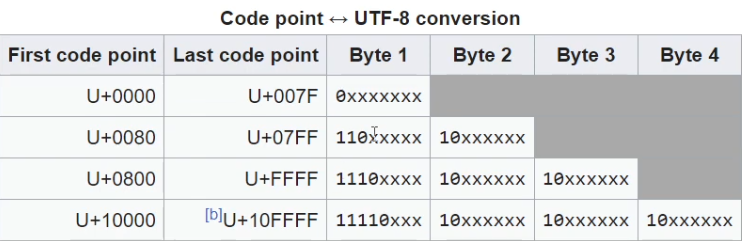
\includegraphics[scale=0.7]{utf8.png}\\
\par UTF-8 и UTF-16 называются кодировками переменной длины. Еще стоит сказать, что сравнение code unit'ов UTF-8 совпадает со сравнением code point'ов, а в UTF-16 нет. Здесь может возникнуть вопрос: зачем вообще использовать что-то кроме UTF-32? Она, в отличие от остальных, не имеет этих проблем, для нее можно быстро посчитать длину строки, не залезая в ее содержимое, и по индексу обратиться тоже можно быстрее. Но не всё так просто. Среди code point'ов есть так называемые combine symbols: всякие точки и кружочки, которые комбинируются с предыдущим символом, но отдельной буквой не считаются. С корейским алфавитом всё ещё хуже: у них разные слоги записываются в строку не подряд, а лепятся в один иероглиф.
\par Еще одно заблуждение -- UTF-16 лучше UTF-8, так как в ней для большего числа символов определена операция toUpper и toLower. Однако, для разных языков могут быть свои правила перевода в заглавную букву для одной и той же буквы. Даже в пределах одного языка могут быть две маленькие буквы, соответствующие одной большой букве (греческая сигма). А еще может быть как в немецком языке: до недавнего времени маленькая буква eszett при капитализации становилась двумя заглавными S. При этом, чтобы перевести в маленькие буквы две заглавные S, нужно знать правила немецкого языка.\\
\par Давайте скажем пару слов про имена файлов. Это не строчки. На линуксе именем файла является любая последовательность байт, не содержащая нулевого байта и слэша. На винде это последовательность 16-битных чисел, не содержащая слэша, двоеточия и т.д. При этом, если пытаться что-то делать с кодировками, назад имя файла уже можно не получить. Поэтому в стандартной библиотеке для работы с именами файловых путей используется path, а не строчка. Еще один момент -- на винде case insensitive файловая система, и многочисленные правила, что считать одной буквой в разном регистре, описаны в огромном файле. И да, этот файл не обновлялся в 2017 году, когда появился заглавный эсцет, поэтому можно создать два файла, названия которых отличаются только регистром эсцета. Также на винде ради совместимости с линуксом сделали возможность создания папки, внутри которой будут case sensitive имена файлов.
\section{Библиотеки}
\subsection{Статические библиотеки}
Статические библиотеки это просто объектные файлы (расширение .o), которые присоединяются во время линковки. Файлы можно объединить в библиотеку с помощью команды ar, библиотечные файлы имеют расширение .a и префикс lib. Чтобы воспользоваться, скажем, библиотекой gtest, нужно чтобы, во-первых, эта библиотека была скомпилированна, и, во-вторых, нужно указать компилятору соответствующую опцию, чтобы он линковался с библиотекой.
\begin{minted}[tabsize=4, autogobble, fontsize=\small]{C++}
	g++ -Igoogletest/googletest/include main.cpp -Lgoogletest/lib -lgtest -lgtest_main
\end{minted}
Здесь флаги -L и -I отвечают за пути к директориям, откуда нужно брать библиотеку, а флаг -l указывает библиотечные файлы, которые будут подключены. К указанному после -l названию добавляется префикс lib и расширение .a. Операции подключения библиотек может выполнять вместо вас vcpkg. Создавать библиотеки позволяет CMake, если прописать в CMakeLists.txt строчку add\textunderscore library.\\
\textit{Замечание.} Иногда линковщику бывает принципиально, в каком порядке указывать библиотеки, а именно библиотека может внутри себя использовать только те, которые идут позже в списке.\\
\textit{Замечание.} Помимо указанных файлов, g++ добавляет файлы, отвечающие за стандартную библиотеку, передавая линковщику соответствующие ключи.\\
\par У статических библиотек есть очевидная проблема: один раз слинкованный бинарник будет потом вечно загружать место на диске и оперативную память, даже когда перестанет быть полезен. Поэтому были придуманы динамические библиотеки.
\subsection{Динамические библиотеки}
Динамические библиотеки имеют расширение .so или .dll. Команда для линковки с динамическими библиотеками выглядит так же как и со статическими, но разница в том, что динамические библиотеки ищутся не в том месте, которое указано с ключом -L, а в специальных местах. Если же мы не хотим перемещать библиотеку в эти места, мы можем либо указать нужный путь в переменной LD\textunderscore LIBRARY\textunderscore PATH, либо воспользоваться особым ключом -rpath. Этот ключ позволяет вписать непосредственно в библиотеку информацию о том, где ее брать. Чтобы путь не был привязан к устройству, у этого ключа есть особое значение, которое говорит брать оттуда, где лежит, \$ORIGIN.\\
\textit{Замечание.} Файл статической библиотеки можно один раз слинковать и потом удалить, а вот shared object файлы удалять нельзя, так как они требуются при каждом запуске программы. С точки зрения ядра при запуске управление передается динамическому загрузчику, он подгружает все необходимые библиотеки, а потом уже управление передается самой программе.\\
\par Вспомним, как работает страничная адресация. Важная деталь, которую следует вспомнить -- операционная система полностью контролирует сопоставление виртуальных и физических адресов для каждой программы, т.е. у каждой программы свое адресное пространство в оперативной памяти, в котором она размещается. Из-за этого динамическую библиотеку нельзя просто положить в память по конкретному адресу: вполне может оказаться, что по этому адресу уже что-то лежит. Хотелось бы, чтобы можно было загружать библиотеку по любому адресу. Однако, внутри библиотеки могут быть команды с абсолютным адресом, такие как lea и mov, и этот адрес может съехать. Чтобы этого не случилось, при создании библиотеки нужно указать ключ -fPIC. Как вообще можно пофиксить проблемы с адресом? Можно узнать, по какому адресу загружается наша библиотека, и сдвинуть все адреса внутри нее на это число. Это называется реаллокация. Это не очень хорошо, так как каждая программа загружает библиотеку по разному адресу, и перед каждой загрузкой придется делать реаллокацию. Тем не менее, на винде сделали именно так, но с небольшой оговоркой: есть base address, куда загружаются библиотеки по умолчанию, а если этот адрес занят -- тогда уж реаллокация. Альтернативный вариант -- компилировать таким образом, чтобы избегать инструкций с абсолютным адресом. Тогда придется найти способ получить адрес инструкции в программе. Можно сделать call и потом pop, но так не делают, потому что это не эффективно: все оптимизации процессора заточены на то, что после call идет ret. Вместо этого вызывается особая функция program counter, которая берет из стека адрес и делает ret. Всего этого геморроя избежали AMD на x64, сделав особую форму lea для относительных адресов. \\
\textit{Замечание.} Когда мы говорим, что редактируем бинарник (например для реаллока), на самом деле редактируется его копия, загруженная в оперативную память.\\
\par Еще одна проблема с тем чтобы загрузить динамическую библиотеку в память -- нужно сделать так, чтобы программа, использующая библиотеку, знала по какому адресу она лежит. Для разных программ виртуальный адрес библиотеки может быть разным. На винде просто добавляют в начало бинарника таблицу с указателями на функции загружаемых библиотек (Import Address Table). При этом компилятор по умолчанию не знает, что для вызова библиотечных функций нужно идти в эту таблицу, поэтому линковщик генерирует код, который перенаправляет вызов функции, чтобы она получала из таблицы адрес и вызывала по этому адресу.\\
\textit{Замечание.} Если используется linked-time оптимизация, ничего не перенаправляется, а сразу вызывается нужная табличная функция.
\par На винде по умолчанию никакие библиотечные функции не видны снаружи, поэтому, чтобы программа могла их увидеть, их нужно либо перечислить в разделе EXPORT в .def файле, либо пометить в самом коде как dllexport.\\
\par Иногда линковщик работает с динамическими библиотеками не совсем так как с обычными объектными файлами. Например, это касатется inline функций. Обычный линковщик берет все экземпляры inline функции и просто выкидывает лишние, но динамический загрузчик оставляет библиотеке и программе их собственные экземпляры функции, он вообще может не знать что они inline. Из-за этого происходит нарушение стандарта, согласно которому у всех объектов линковки должен быть одинаковый адрес inline функции. Еще один момент: в отличие от функций, глобальным переменным адресную табличку не завезли, поэтому пользоваться ими можно только с помощью dllexport/dllimport и extern. Адреса функций тоже будут браться некорректно без dllexport, так как будет браться адрес заглушки, вызов которой перенаправляется через таблицу адресов. По этой причине на винде далеко не любой код можно сделать динамической библиотекой. \\
\subsection{Shared Objects в Linux}
В linux хотели, чтобы любой код можно было превратить в динамическую библиотеку. Из-за этого у gcc есть ряд ограничений при использовании fPIC. Рассмотрим такой код:
\begin{minted}[tabsize=4, autogobble]{C++}
	int sum(int, int);
	
	int (*get_sum())(int a, int b) {
		return &sum;
	}
\end{minted}
При обычной компиляции просто генерируется код, берущий адрес функции, ничего необычного. Однако, при использовании вышеупомянутого флажка, ассемблерный код пытается прочитать указатель на функцию из памяти, использовав в качестве адреса регистр rip. Так выглядит проход через Import Address Table, и он используется для адресов абсолютно всех функций, только в линуксе эта табличка называется Global Offset Table (GOT) и больше ничем не отличается. Еще на винде есть такая фича как отложенная загрузка: библиотека загружается в рантайме непосредственно перед вызовом функции оттуда, чтобы, если ничего не вызывается, можно было ее не загружать. В линуксе тоже есть эта фича. Она может быть полезна также если мы вызываем функции из новой версии библиотеки, которых нет в старой, тогда можно просто заифать этот вызов. Также есть способы загружать функции библиотеки напрямую с помощью функции dlopen. В момент загрузки библиотеки в линуксе можно наблюдать как адрес функции меняется с адреса заглушки на настоящий библиотечный адрес. \\
\par С переходами к адресам библиотечных функций у линукса ситуация почти точь-в-точь как на винде, вот поясняющая картинка:\\
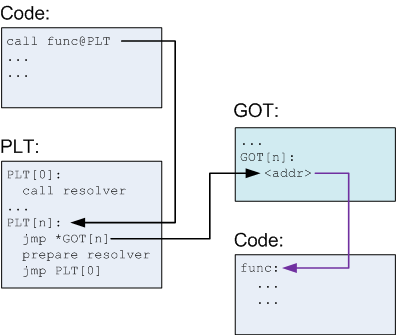
\includegraphics[scale=0.65]{plt.png}\\\\
Когда в коде генерируется тело библиотечной функции, туда вставляется заглушка: набор инструкций PLT, который делает переход на таблицу адресов GOT и достает нужный указатель. В таблице нет ничего интересного кроме набора адресов для соответствующих библиотечных функций, а сами эти функции лежат в коде библиотеки. Есть еще вариант, когда адрес в GOT ссылается на вторую строчку кода PLT <<prepare resolver>>. Это конфигурация в случае когда резолвер еще не вычислил адрес функции после загрузки библиотеки, т.е. когда функция вызыватся первый раз. Для справки, резолвер -- часть кода динамического загрузчика.\\
\par Есть один прикол, связанный с загрузкой функций динамической библиотеки. Если есть несколько экземпляров одной и той же функции, берется первый встреченный. Из-за этого можно сделать так называемый перехват маллока: написать shared object, который переопределяет маллок, выполняя слежение за вызовами, и сказать загружать этот so перед всеми остальными. Это называется interposition, и оно порождает кучу проблем. Например, если функцию можно интерпозить, ее нельзя инлайнить. Это не касается static и inline функций, потому что inline функции всегда одинаковые для всех единиц трансляции, а static функции локальные. Вообще это просто ужасно, потому что в библиотеке может быть куча мелких функций, которые не используются за пределами библиотеки, и хорошо бы их заинлайнить. Для этого в gcc придумали attribute visibility, с помощью которого можно добиться эффекта, противоположного виндовому dllexport, т.е. сказать, что функция не видна снаружи библиотеки. Если применить hidden visibility и использовать ключ, который заставляет напрямую обращаться к GOT и пропускать PLT, можно добиться обычных вызовов как в статических библиотеках.\\
\par Так что же все-таки лучше: статические или динамические библиотеки? Во-первых, код со статическими библиотеками исполняется быстрее, так как не нужно делать никакие реаллокации. Во-вторых, статические библиотеки сразу во время компиляции подсоединяются к исполняемому файлу, и впоследствии получается полностью самодостаточный бинарник. Этот бинарник можно будет запускать хоть через 100 лет, так как он уже содержит внутри себя все необходимое, тогда как приколы динамического загрузчика могут поменяться, и загрузить какую-то библиотеку динамически может оказаться невозможно, если она не обновлялась. В то же время динамические библиотеки намного легче редачить, так как перекомпилировать придется только саму библиотеку, а не все огромные бинарники, которые ее содержат. Особенно критично это для разработчиков дистрибутивов, которые не хотят выкатывать заново весь дистрибутив. Также динамические библиотеки позволяют экономить память, так как можно иметь одну загруженную библиотеку на несколько программ. Еще один забавный бонус -- из-за использования динамических библиотек куски кода разбредаются по памяти и это запутывает злоумышленников :)
\section{Концепты}
\subsection{Мотивация}
Смысл концептов очень прост: когда класс принимает шаблонный тип, разработчик подразумевает, что далеко не любой тип ему подойдет (например тип без деструктора -- довольно странный выбор в большинстве ситуаций), но если просто написать шаблонный параметр, с точки зрения языка туда можно подставить что угодно. До появления концептов использование запрещенных типов приводило к самым разнообразным и зачастую нечитаемым ошибкам компиляции, например попытка запихать в вектор тип без деструктора приводила к ошибке в функции destroy\textunderscore at у аллокатора. Еще одна причина использования концептов -- наложить ограничения на перегрузку функции, например как в следующем коде:
\begin{minted}[tabsize=4, autogobble]{C++}
	template <typename T>
	struct vector {
		void assign(size_t n, T const& value) {}
		
		template <typename It>
		void assign(It first, It last) {}
	}
\end{minted}
Здесь в качестве It с точки зрения компилятора не обязан быть итератор, поэтому эта перегрузка может выбраться в том случае, когда должен быть первый вариант. Как все уже знают, это решается с помощью всеми любимого SFINAE, но хочется иметь механизм языка, который сделали специально для этих целей (SFINAE изначально вообще не предназначалось для такого использования). Также SFINAE весьма тяжелая вещь для компилятора (google the rule of Chiel), а еще оно всё ещё выдает нечитаемые ошибки. Еще можно пользоваться if constexpr, но такой код нельзя расширить без залезания в тело функции. Наконец, есть проблема, которая не решается даже SFINAE. Рассмотрим функцию, которая принимает различные типы, удовлетворяющие или неудовлетворяющие свойствам A, B, C.
\begin{minted}[tabsize=4, autogobble]{C++}
	template <typename T>
	std::enable_if_t<A<T>, void> 
	foo(T&&) {}
	
	template <typename T>
	std::enable_if_t<A<T> && B<T>, void> 
	foo(T&&) {}
	
	template <typename T>
	std::enable_if_t<A<T> && B<T> && C<T>, void>
	foo(T&&) {}
\end{minted}
Согласно обычным правилам перегрузок, если есть несколько подходящих перегрузок, выбирается самая близкая к переданному типу, т.е. всегда когда есть вариант, однозначно превосходящий другие, это не амбиг и не ошибка. В данном случае, если T удовлетворяет всем трем условиям, последняя специализация всегда строго лучше предыдущих двух, однако SFINAE так не работает. Для него все кандидаты, в которые можно подставить тип, являются одинаково валидными, поэтому нам пришлось бы для двух первых специализаций писать также требование, чтобы условия, которые не упомянуты в этой специализации, обязательно не выполнялись, и только тогда это станет работать. А вот как сделать такое с концептами, легко и просто:
\begin{minted}[tabsize=4, autogobble]{C++}
	void advance(std::input_iterator auto& iter, 
				 std::integral auto& dist) {
	}
	
	void advance(std::forward_iterator auto& iter, 
			     std::integral auto& dist) { 
	}
	
	void advance(std::bidirectional_iterator auto& iter, 
				 std::integral auto& dist) { 
	}
	
	void advance(std::random_access_iterator auto& iter, 
				 std::integral auto& dist) { 
	}
\end{minted}
И здесь уже будет выбираться самая лучшая перегрузка при наличии нескольких подходящих.
\subsection{Прототип концептов в C++11}
При разработке концептов встал вопрос, должны ли они быть explicit или implicit, то есть нужно ли специально прописывать в классе, к примеру, является ли он destructible, или достаточно просто написать деструктор. В пользу первого варианта обычно приводят ситуации, когда у разных классов есть метод с одинаковым названием, который делает совершенно разные вещи, и из-за этого они оба могут попасть под действия одного implicit концепта, что нехорошо. С другой стороны, для explicit концептов нужно заморочиться, чтобы они сработали, и программисты зачастую не понимали, что они сделали не так. Из-за этого впоследствии перешли к implicit концептам. Explicit всё ещё можно встретить в итераторах (вспомните iterator category), так как считается, что ++ у input и у forward итераторов делают разные вещи.
\par Также в какой-то момент возник вопрос, нужно ли концептам делать definition checking. Когда мы пишем ограничение на тип, его можно рассматривать двумя способами. Первый -- считать это ограничением на передаваемый тип, т.е. относить ограничение к вызывающему коду. Второй -- считать концепт ограничением на код функции, т.е. внутри функции нельзя пользоваться свойствами типа, если у типа, удовлетворяющего концепту, их нет. Этот вариант и называется definition checking. К сожалению, у него есть две серьезные проблемы. Первая, очевидно, скорость компиляции. Вторая -- возможно, мы захотим делать отладочный вывод, но поскольку не у каждого типа, подходящего под концепт, есть возможность выводиться в офстрим, definition checking нам это заблокирует, даже если мы не собирались передавать туда плохие типы. И да, на момент создания концептов никаких if constexpr не было, а то бы они решили эту проблему. Еще неясно, как организовать взаимодействие обычных шаблонов с definition checking, потому что прикол шаблонов как раз в том, чтобы отложить генерацию тела функции на момент инстанцирования типа, а нет тела -- нет дела, в смысле definition checking'а. Ну и не сделали definition checking в итоге.
\par Третий момент -- concept map'ы, от которых тоже отказались в процессе разработки. Это такая штука, которая позволяла вручную установить, кто конкретно удовлетворяет концепту, например сказать, что у стека, как и у вектора, можно делать push\textunderscore back, только у него вместо этого просто push. Однако, это сильно портило автоматическое определение приоритетов у концептов. Теперь, если концепт A был менее специализированный чем концепт B, предлагалось писать специальный мап, что все типы, удовлетворяющие B, также удовлетворяют A. 
\par Последний момент -- концептуализация стандартной библиотеки. Изначально существовал концепт, который требовал от типа наличия всех шести операторов сравнения, но для какого-нибудь сета достаточно было только оператора меньше, поэтому, чтобы сохранить поведение сета, ему сделали еще один концепт только с оператором меньше. Таким образом стало появляться много мелких более слабых версий существующих концептов. Всё это вместе с предыдущими пунктами привело к тому, что прототип концептов из С++11 в язык вводить не стали, а сделали другие концепты.
\subsection{Концепты в C++20}
Концепт.
\begin{minted}[tabsize=4, autogobble]{C++}
	template <typename T>
	concept destructible = std::is_nothrow_destructible_v<T>;
\end{minted}
С виду концепты -- это просто предикаты, которые могут быть true или false в зависимости от переданного типа. Но на самом деле их возможности гораздо шире.
Есть три формы использования концепта:
\begin{minted}[tabsize=4, autogobble]{C++}
	template <typename T>
	requires destructible<T>
	void foo(T&) {}
	
	template <destructible T>
	void bar(T&) {}
	
	void baz(destructible auto&) {}
\end{minted}
Еще можно использовать концепты от нескольких параметров таким образом:
\begin{minted}[tabsize=4, autogobble]{C++}
	template <typename U, std::convertible_to<U> V>
	void bar(U, V const&) {}
\end{minted}
Здесь при использовании концепта от нескольких параметров тип, на который он налагается, как бы ставится первым параметром при проверке концепта.
\par У концептов из С++20 есть такая замечательная вещь, как ограничение на выражения, т.е. тип удовлетворяет концепту, если его можно подставить в выражение, и это будет валидно.
\begin{minted}[tabsize=4, autogobble]{C++}
	template <typename T>
	concept ordered = requires(T x)
	{
		// simple constraint
		x.foobar();
		// type constraint
		typename T::value_type;
		// compound constraint
		{x < x} -> std::convertible_to<bool>;
		{x < x} noexcept -> std::same_as<bool>;
		// nested constraint
		requires std::destructible<T>;
	}
\end{minted}
Simple constraint -- просто проверка валидности выражения. Type constraint -- проверка наличия зависимого типа. Compound constraint позволяет не только убедится в валидности выражения, но и в том, что результатом выражения будет определенный тип. Наконец, nested constraint это проверка на удовлетворение другого концепта внутри нашего концепта.
\par Давайте посмотрим, как концепты позволяют выбрать более специализированную перегрузку. Чтобы это осуществилось, один концепт должен полностью включать в себя требования другого концепта. Так и есть: концепт signed\textunderscore integral включает в себя концепт integral. Впрочем, гениальность компилятора дальше этих простых проверок не распространяется: например, он не понимает, что массив длины больше 7 более специализирован чем массив длины больше 5. Невозможность делать такие проверки за адекватное время связана с какими-то там свойствами исчисления предикатов или еще чего-то, у меня E по матлогу) Набор синтаксических конструкций, которые компилятор может использовать для ранжирования перегрузок, ограничивается И, ИЛИ, скобками и вложенными концептами. Все, что не является чем-то из этого, называется атомарными констрейнтами. Например, атомарный констрейнт это условие true. В атомарные констрейнты компилятор не лезет. Из-за этого в следующем коде нет амбига, выберется вторая перегрузка:
\begin{minted}[tabsize=4, autogobble]{C++}
	template <typename T>
	requires std::destructible<T>
	void foo() {}
	
	template <typename T>
	requires std::destructible<T> && true
	void foo() {}
\end{minted}
На самом деле вместо концепта destructible можно использовать просто соответствующий трейт is\textunderscore destructible\textunderscore v, но! для атомик констрейнта компилятор не может понимать, что он совпадает с другим таким же констрейнтом, а значит будет амбиг! Также если концепт определен прямо в выражении requires, он становится атомик констрейнтом и с ним происходит то же самое.
\par С помощью концептов крайне легко осуществлять SFINAE-friendliness. Кстати, обращаю ваше внимание, что при использовании SFINAE в функциях класса надо добавить хотя бы один параметр помимо дефолтного typename = enable\textunderscore if\textunderscore t..., потому что значение этого параметра вычислится на этапе подстановки типов в самом классе и функция перестанет быть шаблонной. Вот как нужно правильно делать SFINAE-friendliness (в данном случае сохранение дефолтного конструктора) на SFINAE:
\begin{minted}[tabsize=4, autogobble]{C++}
	template <typename F, typename S>
	struct pair {
		F f; S s;
		
		template <typename T = S, typename U = F,
				  typename = enable_if_t<conjuction_v<
										 is_default_constructible<T>,
										 is_default_constructible<U>>>>
		pair() : f(), s() {}
	};
\end{minted}
А вот как сделать с помощью концептов:
\begin{minted}[tabsize=4, autogobble]{C++}
	pair() requires DefaultConstructible<F> &&
					DefaultConstructible<S> {}
\end{minted}
Также с помощью концептов можно полностью избавиться от дурацкого наследования от enable copy и прочих, и на этом моменте я пошла и уменьшила свой variant на 60 строк, хехе.
\par Когда выполнение одного требования влечет выполнение другого, это называется subsume. Мы хотим, чтобы если тип U равен типу V, из этого следовало что тип V равен типу U, и наоборот. Поэтому концепт same\textunderscore as реализован немного хитрее, чем просто std::is\textunderscore same:
\begin{minted}[tabsize=4, autogobble]{C++}
	template <typename U, typename V>
	concept half_same_as = std::is_same_v<U, V>;
	
	template <typename U, typename V>
	concept same_as = half_same_as<U, V> && half_same_as<V, U>;
\end{minted}
\section{Модули}
Внимание: все фичи, показанные дальше, на момент написания конспекта на 100\% актуальны только для msvc.\\
\par Модули -- одна из самых ожидаемых фич C++20, и в то же время одна из самых сложно реализуемых. В сути своей это альтернатива хэдерам.
\begin{minted}[tabsize=4, autogobble]{C++}
	// ab_sum.ixx
	export module ab_sum;
	
	export int sum(int a, int b) {
		return a + b;
	}
	
	// ab_sum.cpp
	import ab_sum;
	
	int main() {
		std::cout << sum(40, 2) << '\n';
	}
\end{minted}
Сами хэдеры -- явление весьма неприятное, учитывая что там надо постоянно помнить про ODR и не писать определения нешаблонных функций (либо помечать их inline), а также там нельзя использовать static глобальные переменные, потому что они будут свои для каждой единицы трансляции, в которую попадут (если конечно это не то что вы хотите). Да даже помеченная inline функция может нарушить ODR, если в ней будет assert и при этом часть программы будет скомпилированна без ассертов (мы получим две версии одной inline функции, отличающиеся наличием ассерта, а это UB). Ловушка может поджидать даже в самых неочевидных местах, например при хранении std::vector внутри структуры в header'е, потому что в зависимости от сборки (дебаг или релиз) это будет либо обычный вектор, либо debug vector, а у них размеры разные. А еще есть мем, что одни хедера из стандартной библиотеки инклюдят другие, причем на другом компиляторе этого уже может не быть. Даже порядок хэдеров может на многое влиять. И еще: никогда не пишите using namespace std в хэдерах, этот юзинг потом попадет во все cpp файлы!
\par Зависимости между хэдерами это вообще довольно грустно, поэтому разработчики стараются уменьшить их количество. Они делают это двумя способами. Первый -- использование уже знакомого нам pimpl, когда в хэдере в классе хранится указатель на имплементацию класса, причем чтобы хранить указатель, совершенно не нужны библиотеки, необходимые для реализации имплементации. Сами же внутренности имплементации лежат в .cpp, туда же инклюдятся другие хэдера. Чтобы лишний раз не аллоцировать, вместо указателя иногда заводят aligned storage.
\begin{minted}[tabsize=4, autogobble]{C++}
	// mytype.h
	#pragma once
	#include <memory>
	
	struct mytype_impl;
	
	struct mytype {
		mytype();
		mytype(mytype const& other) = delete;
		mytype& operator=(mytype const& other) = delete;
		~mytype();
		
		void foo();
		void bar();
		void baz();
		
		private:
		std::unique_ptr<mytype_impl> pimpl;
	};
	
	// mytype.cpp
	#include "mytype.h"
	#include <string>
	#include <vector>
	
	struct mytype_impl {
		std::string name;
		std::vector<int> data;
	};
\end{minted}
Вот еще один способ с помощью абстрактных классов:
\begin{minted}[tabsize=4, autogobble]{C++}
	// mytype.h
	#include <memory>
	
	struct mytype {
		virtual ~mytype() = default;
		virtual void foo() = 0;
		virtual void bar() = 0;
		virtual void baz() = 0;
	};
	
	std::unique_ptr<mytype> create_mytype();
	
	// mytytpe.cpp
	#include "mytytpe.h"
	#include <string>
	#include <vector>
	
	struct mytype_impl : mytype {
		void foo() override {}
		void bar() override {}
		void baz() override {}
		
		private:
		std::string name;
		std::vector<int> data;
	};
	
	std::unique_ptr<mytype> create_mytype() {
		return std::make_unique<mytype_impl>();
	}
\end{minted}
Хэдера всё равно не самый лучший механизм, потому что даже избавившись от кучи зависимостей и долгого времени компиляции, мы приобрели лишние аллокации, виртуальные функции, бессмысленное наследование и прочую дрянь. Теперь забудем про них и рассмотрим как работать с модулями.
\begin{minted}[tabsize=4, autogobble]{C++}
	export module pair_module;
	
	export struct pair {
		int x, y;
	};
	
	export pair make_pair(int x, int y) {
		return {x, y};   
	}
\end{minted}
Теперь снаружи этого модуля мы можем использовать функцию и структуру. Функция возвращает пару, но что если мы забудем заэкспортить саму структуру пары? Давайте вспомним, как работает компиляция обычных единиц трансляции. Все единицы сначала компилируются самостоятельно, а потом линкуются в один файл. С модулями ситуация немного другая: теперь у нас появляется зависимость от порядка компиляции, так как сначала нужно скомпилировать то, что экспортируется в другие файлы.
\\\\
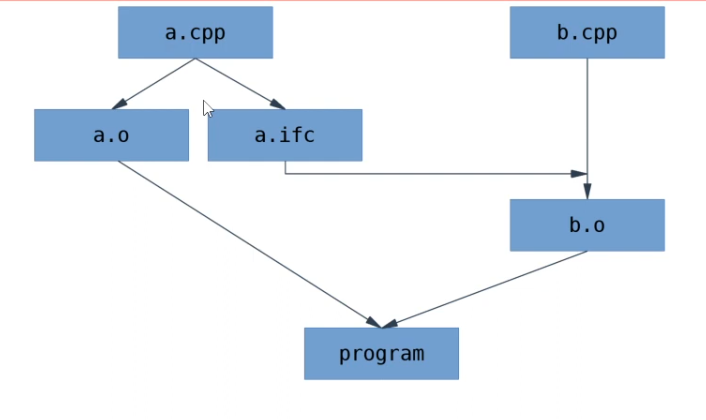
\includegraphics[scale=0.65]{module_compile.png}\\
Здесь видно, что все экспортируемые из модуля штуки помещаются в специальный файл .ifc, из которого потом попадают в другие файлы во время их трансляции. Какой формат файла .ifc? Это бинарник, потому что из него можно импортировать лениво. К сожалению, сделать общий формат этого бинарника для всех компиляторов очень сложно, поэтому все компиляторы используют собственный формат. Так что же будет, если забыть заэкспортить структуру? Ну, вы всё ещё сможете пользоваться функциями, которые ее возвращают, передавать результат в качестве аргумента функций, которые ее принимают, записывать результат в auto и даже конструировать с помощью списочной инициализации (фигурные скобки). Однако, вы не сможете обращаться к ней по имени. Такие структуры называются reachable, а те, к которым можно обращаться по имени, называются visible. Вне модулей пример reachable структуры -- классы лямбд. Однако, если поместить структуру в анонимный неймспейс, она станет не просто локальной, а настолько локальной, что функции, которые ей пользуются, нельзя будет экспортить.
\par Если мы хотим заэкспортить несколько сущностей, надо написать экспорт с фигурными скобками, и в эти скобки все их засунуть. Также можно в одном модуле импортить что-то из другого модуля и экспортить это содержимое дальше с помощью export import.
\par Модули могут ухудшить скорость компиляции по сравнению с хедерами, потому что они добавляют зависимость от порядка компиляции, который мешает параллелить. И тут придумали module implementation unit, который в своей идее подозрительно похож на .cpp файл. Он им на самом деле и является, только в начале файла надо написать module и имя модуля (без export). В этом юните пишут реализацию функции, а в просто модуле тогда только декларацию. Просто модуль называется primary module interface unit и имеет расширение .ixx. Но почему нам вообще нужно писать в начале сппшника, к какому модулю он принадлежит? Всё дело в strong ownership model: если в двух модулях есть две функции или структуры с одинаковым названием, то они разные.
\par Из-за вышеупомянутой модели функции в модулях нельзя перетаскивать из одного модуля в другой, не ломая при этом совместимость. Но что делать, если вы захотели разделить огромный модуль на мелкие части? Для этого существуют partition. Partition это дополнительная часть в имени модуля, которая пишется после двоеточия. Partition не видны снаружи, а линковщик считает, что функции из разных partition все равно находятся в одном модуле, как если бы partition не было. Partition бывают внешние и внутренние. Внешние partition находятся в отдельных файлах .ixx, их импортят и одновременно экспортят наружу. Внутренние partition находятся в файлах .cpp, их только импортят.
\begin{minted}[tabsize=4, autogobble]{C++}
	//ab26-foo.ixx
	export module ab26:foo;
	
	export void foo() {}
	
	//ab26-internal-part.cpp
	module ab26:internal_part;
	
	void ab26_internal_func() {}
	
	//ab26.ixx
	export module ab26;
	export import :foo;
	import :internal_part;
	
	export void bar() {
		ab26_internal_func();
	}
\end{minted}
Представим, что мы хотим ситуацию, когда наружу из модуля торчит только объявление структуры, а ее определение спрятано. Для этого есть особый синтаксис:
\begin{minted}[tabsize=4, autogobble]{C++}
	export module ab27;
	
	export struct pair;
	
	module :private; // private module fragment
	
	struct pair {
		int x, y;
	}
\end{minted}
Мы хотим от модулей совместимости с хэдерами, однако, если мы попытаемся пользоваться хэдером внутри модуля, все содержимое этого хэдера теперь будет принадлежать модулю, в отличие от того же самого содержимого, которое заинклюдили в обычной программе. Для этого придумали global module fragment. Это место в коде модуля до слов export module..., в котором пишут инклюды.
\begin{minted}[tabsize=4, autogobble]{C++}
	module; // global fragment start
	#include <vector>
	export module ab32; // global fragment end
	
	export std::vector<int> foo() {
		return {1, 2, 3};
	}
\end{minted}
Теперь представим, что у нас есть крутая модульная программа, которая хочет использовать С-шную библиотеку, написанную на хэдерах. Один из способов красиво это сделать -- заинклюдить библиотеку в глобальном фрагменте, а потом заэкспортить юзинги интересных нам функций.
\begin{minted}[tabsize=4, autogobble]{C++}
	module;
	#include <cerrno>
	#include <cstdio>
	export module ab33;
	
	export {
		using ::FILE;
		using ::fopen;
		using ::fclose;
		using ::fread;
		using ::fwrite;
		using ::fseek;
	}
\end{minted}
Стоит еще сказать, что для хэдеров std есть соответствующие скомпилированные модули, которые можно заимпортить так:
\begin{minted}[tabsize=4, autogobble]{C++}
	import <vector>;
\end{minted}
\textit{Замечание.} Есть модуль, соответствующий всей стандартной библиотеке, он так и называется -- std.\\
\textit{Замечание.} Если импортить модуль std, некоторые имена, такие как имена целочисленных типов, могут отсутствовать в глобальном неймспейсе, и станут доступны только через квалификатор std. Чтобы не сломать код, где не используются квалификаторы, нужно вместо std импортить особый модуль std.compat.\par
Еще стоит напомнить, что в структурах все функции автоматически inline, однако, для модулей это не имеет особого смысла, поэтому в модулях их не помечают inline. Также модули дружат с шаблонами, и теперь можно раздельно писать объявление и тело шаблонных функций. \\
\section{Ranges}
До C++20 передать в алгоритм сортировки контейнер было нельзя, только два итератора. Это было сделано по той причине, что функция сортировки, принимающая контейнер, должна была наложить на него кучу ограничений, а концептов-то не было... Однако, в С++20 уже ничего не мешало сделать функцию сортировки, принимающую контейнер, но чтобы не портить совместимость, редачить стандартную функцию не стали, а добавили библиотеку ranges.
\begin{minted}[tabsize=4, autogobble]{C++}
	// before C++20
	std::sort(v.begin(), v.end());
	
	// C++20
	std::ranges::sort(v);
\end{minted}
Это, во-первых, короче, а во-вторых нельзя передать несовпадающие итераторы. При этом у сортировки ренджей всё ещё есть перегрузка от двух итераторов, а так же есть специальный тип от двух итераторов -- subrange -- который тоже можно передавать в функцию сортировки.\\
\par Помимо сортировки C++20 также предоставил много улучшений (как в плане удобства, так и в плане производительности) для уже существующих алгоритмов в неймспейсе views внутри библиотеки ranges. Старые алгоритмы, такие как filter, transform и т. д. имели просадку в производительности, из-за того что делали много перекопирований. В С++20 придумали новый объект, который позволяет обходиться без перекопирований. Он называется view. Например, view, который возвращает функция filter, позволяет пробежаться по элементам вектора, при этом наступая только на те, которые удовлетворяют заданному предикату. После получения объекта view из него можно сконструировать вектор, так как у вектора есть конструктор от двух итераторов. Самое прикольное то, что алгоритмы на views можно последовательно применить к контейнеру с помощью синтаксиса, аналогичного конвейеру в bash:
\begin{minted}[tabsize=4, autogobble]{C++}
	std::vector<int> pipe(const vector<int>& v) {
		return v | std::views::filter(is_divisible_by_3)
				 | std::views::transform(square)
				 | std::views::reverse
				 | std::ranges::to<std::vector<int>>();
	}
\end{minted}
Итак, у нас был один алгоритм, а в библиотеке ranges ему теперь соответствуют целых три. Рассмотрим на примере std::transform:
\begin{minted}[tabsize=4, autogobble]{C++}
	// before C++20:
	// std::transform
	
	// C++20
	// std::ranges::transform        "algorithm"
	// std::ranges::transform_view   "view"
	// std::views::transform         "view adapter"
	
	std::ranges::transform_view view1(vec, square_func);
	auto view2 = vec | std::views::transform(square_func);
\end{minted}
Первый алгоритм делает абсолютно то же самое, что и старый transform, только удобнее в использовании и возможно чуть эффективнее. Вторая запись обозначает объект типа view, который не копирует элементы вектора, но если по нему итерироваться, будет выдавать преобразованные элементы. Он очень хорош, если нам не требуется создавать новый контейнер, а достаточно итерироваться по нужным элементам в нужном порядке. Последний вариант это по сути функция, которая принимает вектор и возвращает view.
\par Помните, как при разработке концептов возникла проблема, что навесить на сортировку требование наличия всех шести операторов сравнения было нельзя, так как до этого требовался только оператор меньше? В ranges это исправили, и теперь сортировка требует все шесть операторов.
\par View adapter на самом деле довольно умный: если применить views::reverse к объекту reverse\textunderscore view, получится не дважды реверснутый view, а просто view на исходный вектор. Именно поэтому стоит использовать адаптеры, а не конструировать вьюхи в явном виде, как во второй записи.\\
\par Каждый любитель написать свою библиотеку вьюх должен задаться рядом вопросов, на которые нужно уметь ответить, чтобы вьюхи получились эффективными и качественными. Представим, что у нас есть вектор v и вьюха r, полученная применением views::reverse к v. 
\begin{enumerate}
	\item Является ли r копируемым? Если да, то за какое время?
	\item Разрешается ли r жить дольше чем оригинальный вектор v, на котором он был создан? А если бы v был парой итераторов?
	\item Можно ли менять элементы r и будут ли при этом меняться элементы v?
	\item Изменятся ли ответы на предыдущие вопросы, если v будет rvalue?
\end{enumerate}
При попытке ответить на эти вопросы стоит иметь в виду модель, согласно которой вьюхи это небольшие по памяти объекты, которые не копируют в себя элементы вектора, эдакие ссылки. Введем более точные определения: range -- это что угодно, у чего есть begin() и end(), а view это range, который мувается за O(1). Итак, попробуем ответить:
\begin{enumerate}
	\item Да, r является копируемым и копируется за O(1), так как это просто ссылка. В прицнипе сейчас по стандарту он не обязан быть копируемым, потому что некоторые view хранят некопируемые функциональные объекты, но для большинства вьюх этот ответ все равно справедлив.
	\item View не может пережить range, на базе которого создан, если range был lvalue.
	\item Да, можно, элементы v тогда будут меняться.
	\item Чтобы ответить на этот вопрос, поймем, как работают пайплайны на адаптерах. На самом деле они принимают вьюху, преобразовывают ее и передают дальше, а если вдруг в самом начале им на вход подали range, его превращают во вьюху особым образом. Если range уже вьюха, ничего не делаем. Если это lvalue, возвращаем ref\textunderscore view, который просто ссылается на исходный контейнер. Если это rvalue, возвращаем owning\textunderscore view, который сохраняет range внутри себя.
\end{enumerate}
По историческим причинам в библиотеку ranges добавили возможность иметь begin и end разного типа. Теперь begin и есть begin, а вот end называется sentinel и по факту это просто условие на конец ренджа. Это позволяет иметь бесконечные ренджи, например рендж натуральных чисел iota. Тип сентинела можно указывать при работе с ренджом, передавая ему разнообразные условия, например нулевой символ (для обозначения конца строки). Однако, реализовать разные типы begin и end оказалось не так просто. Раньше, когда мы, скажем, копировали рендж, мы всегда знали, что по завершении копирования begin() изначального контейнера станет равным end(), поэтому можно было вернуть только итератор на начало скопированной последовательности. Теперь же нужно возвращать итератор копируемой последовательности тоже. Для этого возвращается структурка copy\textunderscore result, которая как раз содержит в себе два итератора. При этом, если в функцию изначально передавалось rvalue, первый итератор будет иметь тип dangling, то есть заглушка вместо невалидного итератора на мертвый контейнер. \\
\textit{Замечание.} Рендж, который имеет одинаковые типы begin() и end(), называется common range.
\par В C++20 немного изменили поведение итераторов. Во-первых, начиная с forward iterator все итераторы обязаны были возвращать lvalue, но некоторые вьюхи (iota, transform) просто не могут себе это позволить. Поэтому ввели еще одну характеристику iterator\textunderscore concept, согласно которой итераторы iota и transform являются random access, но согласно старой iterator\textunderscore category они просто input итераторы. Еще появились contiguous итераторы, которые как random access, но элементы еще и лежат в памяти подряд. 
\section{Профилировщики}
Профилировщики -- это программы, которые позволяют оценить, в каких своих местах программа проводит сколько времени. Это очень полезная вещь для поиска проблем с производительностью для последующего их исправления. Обычно в сколько-нибудь сложной программе чрезвычайно сложно на глаз понять, какие части недостаточно быстры или вызываются слишком много раз. Профилировщики помогают не только найти проблему, но и убедиться, что она была устранена.
\par По своим принципам работы профилировщики делятся на трассирующие и сэмплирующие. Первые фиксируют каждый вход и выход из функции, тем самым определяя время, которое проводится в каждом вызове. Они, во-первых, требуют дополнительной предкомпиляции, потому что фиксация вставляется прямо в код, а во-вторых сама трассировка тоже занимает время, поэтому при частых вызовах мелких функций накопится очень большая погрешность. Второй вид профилировщиков просто прерывает программу через равные очень маленькие промежутки времени и смотрит, в какой функции она находится.
\par Из известных профилировщиков можно выделить VTune, DotTrace и perf. VTune разработан интелом, поэтому для их процессоров он может делать анализ на уровне архитектуры, т.е. анализировать такие ситуации как неправильные предсказания переходов, простаивание конвейера, кэш-промахи, долгие обращения к памяти и т.д. Это достигается с помощью специальных счетчиков в процессоре, но у каждого процессора они свои, поэтому использовать профилировщик таким образом на другом процессоре не выйдет. Анализировать эти счетчики можно с помощью прерываний по событию.
\par Профилировщики для отображения результатов требуют компиляции в режиме вывода дебажной информации. В основном это имена функций. Если информации про них будет не хватать, будет выводиться адрес соответствующей инструкции в ассемблере.
\par Поскольку все вышеупомянутые профилировщики сэмплирующие, может сложиться впечатление, что трассирующие профилировщики бесполезны. Это не так: во-первых, они позволяют подсчитать количество заходов в каждую функцию, поэтому ситуации, когда функция очень тяжелая или когда она просто очень часто вызывается, становятся различимы. Во-вторых, они позволяют объединять несколько функций в события и смотреть, в каких логических частях проводится больше всего времени. В-третьих, сэмплирующие профилировщики любят всё усреднять, а ситуации, когда функция ужасно тормозит каждый сотый вызов, они не способны отловить. Короче, все профайлеры важны, все профайлеры нужны :)
\section{Многопоточность}
\subsection{Введение}
Многопоточность -- это разделение одного процесса на части, которые выполняются одновременно. Зачем это вообще нужно? Во-первых, современный компьютер многоядерный, поэтому класть всё исполняться последовательно на одном ядре просто невыгодно. Во-вторых, в некоторых программах есть разделение на логические части (например взаимодействие с вводом/выводом и сложные вычисления), и хотелось бы, чтобы они друг другу не мешались. В-третьих, существуют блокирующие вызовы, которые тормозят всё дальнейшее исполнение программы, даже те её части, которые никак от этого вызова не зависят. Стоит, однако, иметь в виду, что распараллелить программу не так то просто, поскольку есть куча разных нюансов, уникальных для каждой программы. 
Наверно, самая большая проблема многопоточности -- её непредсказуемость. Зачастую поведение программы будет зависеть от того, какой поток первым получил доступ к ресурсам, кому пришлось их освобождать и т.д. Поэтому дебажить это фактически невозможно :) Итак, добро пожаловать в ад.
\par Для начала научимся создавать поток. Это делается с помощью библиотеки thread.
\begin{minted}[tabsize=4, autogobble]{C++}
	#include <iostream>
	#include <thread>
	
	int main() {
		std::thread th([]
		{
			std::cout << "Hello world!\n";
		});
		
		th.join();
	}
\end{minted}
Здесь поток, который мы создаем, отделяется от основного потока. Операция join заставляет основной поток ждать, пока наш поток отработает, и потом закрыть его. Помимо join есть еще detach, который отвязывает наш поток полностью и он исполняется независимо, а основному потоку не приходится его ждать. Для тех, кто шарит в bash, можно провести аналогию с запуском в фоновом режиме. Однако, в нашей программе hello world нельзя просто так заменить join на detach. Разберемся поподробнее, как эти два метода устроены изнутри. У объекта thread есть два состояния: привязанный к основному потоку и висящий в воздухе. Операция join дожидается завершения потока и только потом переводит его в висящий режим. Операция detach делает это изначально, не дожидаясь завершения. Прикол в том, что во втором случае main может спокойненько завершиться без нашего потока и начать разрушать глобальные переменные, пока поток ими всё ещё пользуется. Одной из таких переменных является cout. Будет очень печально, если он внезапно умрет в середине вывода, не так ли? Вообще, лучше не использовать detach, потому что это означает потерю контроля над потоком. Ну разве что только если ваш поток вообще не использует никакие глобальные переменные, но это редкий случай. А что произойдет, если мы не сделаем ни join, ни detach? Это считается ошибкой и программа завершится аварийно. Почему в этом случае не делается автоматический detach понятно, а join не делается, потому что некоторые потоки предназначены чтобы вечно висеть где-то на фоне и ждать команд, поэтому, если использовать на них join, это навсегда повесит программу. Вот и выбрали не делать ничего и просто кидать ошибку. В С++20 появился крутой супер-поток jthread, который джойнится автоматически, и при этом имеет механизм, чтобы не висеть вечно.
\par Поток, который висит, можно прервать, однако, в стандартной библиотеке нет способа прервать его без разрешения самого потока, можно только вежливо попросить и надеяться, что он послушается. Это сделано по той причине, что у потока могут быть какие-то личные ресурсы, которые может закрыть только он, и если его прервать, они утекут. Либо поток будет прерван в тот момент, когда он временно нарушил какой-то инвариант, что тоже плохо. Поэтому потоки в jthread должны либо завершаться сами после отработки, либо обрабатывать прерывание, пришедшее снаружи, в случае если они исполняют бесконечный цикл.
\begin{minted}[tabsize=4, autogobble]{C++}
	std::jthread th([] (std::stop_token const& tok) {
		while (!tok.stop_requested()) {
			// ...
		}
	});
\end{minted}
\textit{Замечание.} Насильно прерывать поток опасно, а насильно прерывать процесс -- нет. Это связано с тем, что процессы все друг от друга изолированны, и ОС может убить процесс, не повредив другим, при этом она знает, какие ресурсы выделял процесс.
\subsection{Потоки и общие данные}
Создавать потоки оказалось довольно просто, но самая сложная часть -- контролировать их взаимодействие. Рассмотрим такую функцию изменения банковского счета:
\begin{minted}[tabsize=4, autogobble]{C++}
	std::array<int, 10000> accounts;
	
	void transfer(size_t from, size_t to, int amount) {
		if (accounts[from] < amount)
			throw std::runtime_error("insufficient funds");
		
		accounts[from] -= amount;
		accounts[to]   += amount;
	}
\end{minted}
Довольно простая функция, что может пойти не так? Если код запускается с одного потока, мы точно знаем, что счёт не может уйти в минус, так как сначала идет проверка. Но что если два потока переводят деньги от одного пользователя? Оба успели проверить, что им хватит на одно вычитание, затем оба вычитают и на счете остается отрицательное число, так как между проверкой и вычетом одного потока другой уже успел встрять и вычесть свою сумму, но проверка для первого потока уже была сделана. Если исполнение программы зависит от того, в каком порядке будут выполнены инструкции разных потоков, это называется race condition. Вообще, некоторые операции лучше считать единой операцией: то есть пока всё не выполнится, другие потоки не смогут увидеть результат. Это называется атомарная операция. Вообще, с точки зрения C++ -= это атомарная операция, но мы можем представить что было бы, если бы это были три разные операции: чтение из памяти, вычисление и запись в память. Тогда результат тоже мог бы быть некорректным. Вот теперь нам хочется, чтобы был способ выделить какую-то функцию и сказать, что она целиком является атомарной. Для этого в стандартной библиотеке есть структура mutex и его методы lock и unlock.
\par У mutex'а есть два состояния: залоченный и разлоченный. Операция lock делает следующее: если mutex не залочен, он лочится, а если залочен, ждет пока он разлочится и тогда лочит. Операция unlock просто анлочит мьютекс. Соответственно код, который находится между локом и анлоком, может исполняться только одним потоком одновременно. 
\begin{minted}[tabsize=4, autogobble]{C++}
	std::array<int, 10000> accounts;
	std::mutex accounts_mutex;
	
	void transfer(size_t from, size_t to, int amount) {
		accounts_mutex.lock();
		
		if (accounts[from] < amount)
			throw std::runtime_error("insufficient funds");
		
		accounts[from] -= amount;
		accounts[to]   += amount;
		
		accounts_mutex.unclock();
	}
\end{minted}
В этом коде всё ещё есть ошибка: если один поток закроется в этой функции а потом кинет исключение, мьютекс останется залоченным навсегда. Поэтому применяют lock\textunderscore guard. Это класс, который в конструкторе делает lock, а в деструкторе unlock. Теперь мы вооружены RAII, и нам больше не надо беспокоиться об исключениях.
\begin{minted}[tabsize=4, autogobble]{C++}
	void transfer(size_t from, size_t to, int amount) {
		std::lock_guard guard(accounts_mutex);
		
		if (accounts[from] < amount)
			throw std::runtime_error("insufficient funds");
		
		accounts[from] -= amount;
		accounts[to]   += amount;
	}
\end{minted}
\textit{Замечание.} Стоит подчеркнуть, что когда мы заводим мьютекс, он относится не к функции, а к данным, и все функции, работающие с этими данными, должны будут лочить этот мьютекс.
\par Многие могут спросить, а чем вообще функции с мьютексом будут отличаться от просто последовательного исполнения? Какой смысл тогда вообще что-то распараллеливать? На самом деле секция с мьютексом может занимать намного меньше времени, чем какие-то независимые участки кода, которые не пользуются общими данными. Тем не менее, лучше всё равно стараться использовать мьютекс как можно меньше. Давайте попробуем улучшить параллельность в нашем примере с банком. Обратим внимание, что у нас 10000 независимых счетов, а использование мьютекса лочит их все, когда в реальности мы лишь хотим не допустить одновременное использование одного из 10000 счетов. Решение -- завести мьютекс на каждый счет.
\begin{minted}[tabsize=4, autogobble]{C++}
	struct account {
		int balance;
		std::mutex mutex;
	};
	
	std::array<account, 10000> accounts;
	
	void transfer(size_t from, size_t to, int amount) {
		std::lock_guard guard_from(accounts[from].mutex);
		std::lock_guard guard_to(accounts[to].mutex);
		
		if (accounts[from] < amount)
			throw std::runtime_error("insufficient funds");
		
		accounts[from] -= amount;
		accounts[to]   += amount;
	}
\end{minted}
Представим, что в коде выше один поток хочет перевести деньги со счета 1 на счет 2, а второй со счета 2 на счет 1. Первый залочил счет 1, и сразу же после него второй залочил счет 2. Дальше первый хочет залочить счет 2, но он уже залочен, поэтому приходится ждать, пока его разлочат. А второй хочет залочить счет 1, но там тоже уже залочено, и в итоге второй тоже сидит ждет. В итоге они оба сидят ждут друг друга, и никто из них не может сдвинуться с места. Такая ситуация называется deadlock.
\par Чтобы анализировать дедлоки, можно построить граф. В графе ребро $A\rightarrow B$ существует, если поток, удерживая мьютекс $A$, может пытаться залочить мьютекс $B$. Если в полученном графе будет цикл -- поздравляем, дедлок. И наоборот: если цикла нет, дедлока не будет. А теперь представим, что в нашей программе мы всегда сначала лочим более маленький номер, а потом более большой. Тогда у нас есть ребра только из меньших номеров вершин в большие, значит можно сделать топологическую сортировку, просто расположив вершины-мьютексы по возрастанию, значит граф ациклический. 
\begin{minted}[tabsize=4, autogobble]{C++}
	void transfer(size_t from, size_t to, int amount) {
		assert(to != from);
		size_t min_acc = std::min(to, from);
		size_t max_acc = std::max(to, from);
		std::lock_guard guard_min(accounts[min_acc].mutex);
		std::lock_guard guard_max(accounts[max_acc].mutex);
		
		if (accounts[from] < amount)
			throw std::runtime_error("insufficient funds");
		
		accounts[from] -= amount;
		accounts[to]   += amount;
	}
\end{minted}
Проблема с дедлоками существует исключительно из-за того, что, залочив мьютекс, поток не хочет его отпускать. В стандартной библиотеке есть функция std::lock, которая лочит несколько unique lock'ов (объект, аналогичный lock guard, но который может изначально не быть залоченным) и делает это так, чтобы не возникало дедлоков. 
\begin{minted}[tabsize=4, autogobble]{C++}
	void transfer(size_t from, size_t to, int amount) {
		assert(to != from);
		std::unique_lock guard_from(accounts[from].mutex, std::defer_lock);
		std::unique_lock guard_to(accounts[to].mutex, std::defer_lock);
		
		std::lock(guard_from, guard_to);
		
		if (accounts[from] < amount)
			throw std::runtime_error("insufficient funds");
		
		accounts[from] -= amount;
		accounts[to]   += amount;
	}
\end{minted}
\subsection{Многопоточная очередь}
Показательным примером дизайна многопоточной программы является многопоточная очередь. В нашей реализации это просто надстройка над деком из стандартной библиотеки (он не многопоточный). Пусть у нас хранится дек и мьютекс. Рассмотрим такую реализацию методов empty и pop:
\begin{minted}[tabsize=4, autogobble]{C++}
	bool empty() const {
		std::lock_guard guard(m);
		return q.empty();
	}
	
	T pop() {
		std::lock_guard guard(m);
		T result = std::move(q.front());
		q.pop_front();
		return result;
	}
	
	std::deque<T> q;
	std::mutex m;
\end{minted}
Функция empty обычно применяется перед функцией pop, чтобы убедиться, что очередь не пуста, однако можно заметить, что после выхода из empty и до входа в pop lock будет некоторое время опущен, и этого времени быстрому Гонзалезу хватит, чтобы удалить все элементы из очереди либо добавить их, сделав результат empty попросту невалидным. Этот пример показывает, что чтобы сделать класс многопоточным, недостаточно обернуть каждую функцию в lock guard.\par
А что если нам соединить empty и pop в одну функцию, которая будет под одним лок гардом проверять очередь на наличие в ней элементов и возвращать optional, который будет пустым, если удалить не получилось?
\begin{minted}[tabsize=4, autogobble]{C++}
	std::optional<T> try_pop() {
		std::lock_guard guard(m);
		if (q.empty())
			return std::nullopt;
		T result = std::move(q.front());
		q.pop_front();
		return result;
	}   
\end{minted}
Ну хорошо, мы избежали ошибки, но что теперь делать пользователю, у которого не получилось удалить элемент из очереди? Ждать, пока он там появится? Но мы же не хотим делать цикл бесконечных проверок, который будет занимать нам ядро. Для этого есть особый класс conditional variable, который может находиться в состоянии ожидания (активируется методом wait), а может проснуться и уведомить об этом один или все потоки. Мы будем использовать эту переменную, чтобы уведомлять о добавлении элемента в очередь, тем самым прервав ожидание pop'а.
\begin{minted}[tabsize=4, autogobble]{C++}
	void push(T value) {
		std::lock_guard guard(m);
		q.push_back(std::move(value));
		cv.notify_one();
	}
	
	T pop() {
		std::unique_lock guard(m);
		
		while (q.empty())
			cv.wait(guard);
		
		T result = std::move(q.front());
		q.pop_front();
		return result;
	}
	
	std::deque<T> q;
	std::mutex m;
	std::conditional_variable cv;
\end{minted}
Метод wait принимает unique lock и временно анлочит его, пока не придет уведомление, а потом лочит обратно. Зачем мы обернули wait в while? Это для того, чтобы если между моментом, когда прозвенел будильник, и моментом, когда wait снова поднял lock, быстрый Гонзалес почистил только что добавленный в очередь элемент, мы уже с поднятым локом вернулись в начало цикла, увидели что очередь опять пуста, и снова активировали wait. Замечательная особенность wait -- он атомарно, то есть без зазора опускает lock и начинает ждать, то есть нет такого, что в этом промежутке Гонзалес успел что-то запушить, и мы будем ждать пока наполнится и так непустая очередь.\\
\textit{Замечание.} Если мы заменим конкретно в этом примере notify one на notify all, это не будет ошибкой, просто много потоков проснутся только чтобы увидеть, что кто-то уже удалил только что добавленный элемент, и лягут спать дальше. Google thundering herd problem.\\
\textit{Замечание.} Поскольку все используют wait внутри while, ему даже сделали особую перегрузку от лока и предиката, которая просто делает while по предикату.
\par На самом деле notify one не очень дешевая операция, а мы ее в бутылочное горлышко заталкиваем, делая ее с включенным локом. Можно поместить лок в отдельный scope, чтобы notify one делался уже с выключенным локом.
\begin{minted}[tabsize=4, autogobble]{C++}
	void push(T value) {
		{
			std::lock_guard guard(m);
			q.push_back(std::move(value));
		}
		cv.notify_one();
	}
\end{minted}
Может быть еще можно вызывать notify one только когда очередь была пуста и туда что-то добавили? Представим, что у нас спят 10 pop, и тут очень быстро произошли 10 push, так что ни один pop не успел проснуться. При этом первый сделает notify, а остальные 9 уже нет, и 9 pop будут просто спать при полной очереди.
\par Что если мы захотим не только запрещать удалять из пустой очереди, но и запрещать добавлять в переполненную очередь? Для этого можно просто завести второй cv.
\subsection{Atomic}
Помните самый первый пример про race condition? На самом деле этот код некорректен не только с точки зрения правильности работы, но и с точки зрения языка. Дело в том, что согласно memory model языка С++, одновременное чтение и запись или только запись в один участок памяти двумя разными потоками считается undefined behavior, если конфликтующие взаимодействия с памятью не являются atomic. Чтобы как минимум убрать UB из программы (но всё ещё иметь проблемы из позапрошлого параграфа) нужно обернуть int в std::atomic.
\begin{minted}[tabsize=4, autogobble]{C++}
	std::array<std::atomic<int>, 10000> accounts;
\end{minted}
В атомик можно завернуть любой тривиально копируемый тип, и потом с ним делать все его операции. Еще у него есть особая операция exchange, которая позволяет атомарно прочитать старое значение и записать новое. Эта операция может пригодиться если мы, например, реализовываем мьютекс, у которого есть состояние locked и unlocked. При вызове lock мы с помощью exchange можем проверить, было ли у нас состояние unlocked, и тут же заменить его на locked.\\
\textit{Замечание.} Мьютексы всё ещё актуальны: если мы с их помощью гарантируем, что никто не работает с переменной одновременно, нам не нужен атомик.
\par Раз уж мы заговорили про реализацию мьютекса, давайте как раз рассмотрим, как внутри устроена функция lock. Когда мы с помощью exchange убедились, что мьютекс был разлочен, можно его спокойно залочить. Но что если он уже залочен? Как ждать, пока его разлочат?
\begin{minted}[tabsize=4, autogobble]{C++}
	void lock() {
		while (state.exchange(mutex_state::locked) == mutex_state::locked) {
			// wait somehow
		}
	}
\end{minted}
Если делать пустой цикл это называется busy wait и это не очень хорошо, так как потребляет ресурсы процессора. Если делать sleep(1), то в худшем случае lock будет работать на 1 мс медленнее, так как после анлока пройдет еще 1 мс, прежде чем он поймет, что его время пришло. Есть еще всякие sleep(0) и yield, которые говорят операционной системе, что нашему потоку нечем заняться, и пусть вместо него на этом ядре поработает кто-то другой. Это тоже нехорошо, потому что миграция потоков с одного ядра на другое приводит ко всяким кэш миссам, и вообще ОС делает это очень неохотно. Вместо всего этого используется особое API, которое внутри функции wait принимает адрес и ожидаемое значение, и если значение совпадает с значением в адресе, поток засыпает. Функция wake при этом принимает адрес и пробуждает тех, кто вызвал wait по этому адресу. На линуксе это API называется futex. Операции из futex и его виндовского аналога добавили в качестве методов std::atomic в виде уже знакомых нам wait, notify one и notify all.\\
\textit{Замечание.} Это не совсем тот wait, который использовался в conditional variable, поскольку у него, по-впервых, другая сигнатура, а во-вторых wait атомиков заканчивается тогда и только тогда, когда значение действительно изменилось. У cv же бывают spurious wake ups, которые мы обсуждали, когда поместили wait в while. В примере выше, правда, atomic wait тоже внутри while, но по другим причинам. Spurious wake up может также произойти даже без какого-либо notify, просто по вине ОС, но atomic wait это скрывает и не пробуждается.
\begin{minted}[tabsize=4, autogobble]{C++}
	void lock() {
		while (state.exchange(mutex_state::locked) == mutex_state::locked) {
			state.wait(mutex_state::locked);
		}
	}
	
	void unlock() {
		state.store(mutex_state::unlocked);
		state.notify_one();
	}
	
	std::atomic<mutex_state> state;
\end{minted}
Теперь представим ситуацию, когда какой-то поток часто делает lock/unlock, при этом ему не приходится никого ждать. Тогда на каждом анлоке будет вызываться notify one, который будет долго лезть в ОС, хотя в этой ситуации это совершенно не нужно. Чтобы разобраться с этим, понадобится еще одна операция атомиков compare exchange. Она принимает аргументы expected (по ссылке) и desired. Если в атомике expected значение, туда атомарно записывается desired значение и возвращается true, а иначе возвращается false и вместо expected подставляется то, что лежит там на самом деле. Вот как можно реализовать transfer с помощью этой функции:
\begin{minted}[tabsize=4, autogobble]{C++}
	std::array<std::atomic<int>, 10000>
	
	void transfer(size_t from, size_t to, int amount) {
		int old = accounts[from].load();
		
		for (;;) {
			if (old < amount) {
				throw std::runtime_error("insufficient funds");
			}
			if (accounts[from].compare_exchange_weak(old, old - amount) {
				break;
			}
		}
		
		accounts[to] += amount;
	}
\end{minted}
У compare exchange есть два варианта: weak и strong. Отличие weak в том, что он может вернуть false даже когда старое значение совпадает с текущим. Внутри strong используется цикл, поэтому, если вы и так оборачиваете compare exchange в цикл, weak будет работать быстрее.
\par Теперь, чтобы сделать такой mutex, который вызывает notify one только если кто-то ждет, заведем три состояния: мьютекс разлочен, мьютекс залочен без ждущих, мьютекс залочен и какие-то потоки желают сами его залочить. 
\begin{minted}[tabsize=4, autogobble]{C++}
	mutex()
	: state(mutex_state::unlocked)
	{}
	
	void lock() {
		// just for lvalue in compare_exchange
		mutex_state expected = mutex_state::unlocked;
		if (state.compare_exchange_strong(expected, 
		                                  mutex_state::locked_no_waiters))
			return;
		
		while (state.exchange(mutex_state::locked_potential_waiters) 
			   != mutex_state::unlocked)
			state.wait(mutex_state::locked_potential_waiters);
	}
	
	void unlock() {
		mutex_state old = state.exchange(mutex_state::unlocked);
		assert(old != mutex_state::unlocked);
		
		if (old == mutex_state::locked_potential_waiters)
			mutex_state.notify_one();
	}
\end{minted}
Хоть busy wait и плохая практика в общем случае, в реальности иногда мьютексы защищают очень маленькие куски кода, для которых покрутиться немного в цикле дешевле чем идти в операционную систему. Реальные мьютексы прежде чем переходить в системное ожидание немного крутятся в цикле, на случай если их в это время заанлочат. Такая оптимизация называется spinlock. Есть способы показать процессору, что поток находится в спинлоке, чтобы не тратить на него много мощности.
\par Помимо обычного мьютекса есть еще рекурсивный мьютекс, который используется в рекурсивных функциях, ставящих lock в начале каждого вызова. Он хранит счетчик вызовов lock одного потока. Понятно, что для обычного мьютекса дважды делать lock одним потоком нельзя. Есть еще shared mutex, у которого есть разные локи на read (shared lock) и на write (exclusive lock).\\
\par Почему вообще нам нужны атомики вместо обычных интов? Во-первых, даже при одном потоке последовательное исполнение инструкций в задуманном порядке -- иллюзия. Процессор может переставлять их как хочет, если сможет гарантировать, что для одного потока результат останется корректным. А вот если вклинится другой поток -- начнется полный бардак. Даже компилятор может переупорядочивать операции. Во-вторых, на уровне ассемблера даже самые простые инструкции не всегда являются атомарными. Если мы скомпилируем код с атомиками, мы увидим, что вместо инструкции mov используется какая-то другая инструкция. Почему это так? Дело в том, что чтение и более ранняя запись в память могут быть переупорядочены, если они обращаются к разным адресам. Есть категория инструкций, которые переставлять нельзя (locked instructions), и xchg, которую используют вместо mov, как раз к ним относится.
\par Вообще атомики еще должны удовлетворять sequential consistency -- это принцип, согласно которому операции можно расставить как-то на временной оси, чтобы они, выполненные в таком порядке, дали тот же результат, как когда выполнялись параллельно, причем операции в пределах одного потока должны полностью соответствовать своему порядку в программе. Однако, sequential consistent операции на некоторых архитектурах довольно дорогие, да и не всегда нам это нужно. Например, если несколько потоков отлавливают какие-то события и инкрементят счетчик -- какая разница, в каком порядке они его заинкрементили? Чтобы сказать об этом операции инкремента, нужно передать ей дополнительным параметром особое значение relaxed memory order. Его еще можно использовать чтобы записать в атомик значение до начала работы с ним потоков или после окончания.
\begin{minted}[tabsize=4, autogobble]{C++}
	counter.fetch_add(1, std::memory_order::relaxed);
\end{minted}
\textit{Замечание.} Relaxed order разрешает менять операцию местами с другими, но она всё ещё обязана быть атомарной.\\
Еще одно применение memory order -- <<публикация изменений>>. Здесь мы познакомимся с двумя новыми memory order: release и acquire.
\begin{minted}[tabsize=4, autogobble]{C++}
	int value;
	std::atomic<bool> value_ready;
	
	void producer() {
		value = 42;
		value_ready.store(true, std::memory_order::release);
	} 
	
	void consumer() {
		if (value_ready.load(std::memory_order::acquire)) {
			int tmp = value;
		}
	}
\end{minted}
Единственное, что мы не хотим -- чтобы операция присваивания в value исполнилась после обновления значения value\textunderscore ready или чтобы запись value в tmp выполнилось раньше, чем подсчитается условие ифа. В остальном, любые изменения порядка нам подойдут. Можно думать об этой штуке как о мьютексе: release -- аналог unlock, acquire -- lock.\\
\textit{Замечание.} Тут в лекции было сказано, что relaxed order это expert friendly штука, которая улучшает скорость только на некоторых архитектурах (не самых популярных к тому же), поэтому использовать их не рекомендуется. Возможно, это не относится к заданию экзамена с многопоточкой, если оно будет.\\
\par Когда наша программа имеет несколько потоков, которые осуществляют запись в общую память, возникает проблема, которая называется sharing. У каждого ядра есть свой кэш, либо общий кэш на несколько ядер, и приходится тратить длительное время на перекидывание данных между этими кэшами (вспомните modified состояние кэша из курса архитектуры ЭВМ), из-за чего распаралеленная программа работает хуже, чем программа на одном ядре. По этой причине, если у вас есть возможность задать на каких ядрах будет работать, скажем, двухпоточная программа, берите соседние ядра, у них больше общих кэшей. Если потоки работают с разной памятью, но при этом эта память внутри одной кэш-линии, всё равно будет плохо. Это называется false sharing. Аллокаторы стараются так аллоцировать память, чтобы разные потоки попадали в разные кэш-линии. False sharing можно побороть с помощью структур с alignas 64 (размер линии).\\
\par Небольшой бонус: многие люди считают, что volatile это какой-то аналог атомиков. На самом деле, volatile используется для трех случаев: UNIX сигналы, семейство инструкций setjmp/longjmp (С-шная попытка в исключения) и device-mapped memory. Основная цель volatile -- посылать с его помощью сигналы, например сначала сделав a = 1, а потом сразу же a = 2. Для обычной переменной компилятор бы просто убрал первое присваивание, а volatile позволяет сказать, что так делать нельзя. При этом атомик может разрешить эту оптимизацию. И наоборот, в примере с публикацией результатов volatile может переставлять присваивание флага и запись в value, потому что это разные места в памяти. Как видите, к многопоточке volatile не имеет отношения.
\subsection{Многопоточный Signal}
Большинству классов из стандартной библиотеки вообще параллельно на многопоточность (извините), в основном это контейнеры, которые предоставляют контракт <<читать могут все одновременно, а записывать придется под мьютексом, о котором вы должны позаботиться сами>>. В случае с сигналом такое рассуждение не работает, потому что сигнал предназначен для того, чтобы разные пользователи (потоки) одновременно могли реагировать на события. Например, если есть общий лог, куда кто-то хочет выводить сообщения, а кто-то принимать их. Делается сигнал, к которому все желающие его слушать подключают свои слоты, реагирующие на сообшения, а тот, кто будет писать сообщение, просто эмитит сигнал, передав сообщение в виде аргумента. Теперь, когда мы поняли, зачем сигналу встроенная многопоточность, приступим к первому шагу осознания: создадим общий мьютекс на весь сигнал и навесим его на каждую из функций (connect, disconnect, emit/operator()). Однако, рассмотрим такое применение сигнала: пусть у нас есть класс, который выполняет большие вычисления. У него есть мьютекс, который висит на функциях этого класса. Есть сигнал timer, у которого есть connection <<timeout>>. Когда вычисления заканчиваются, вызывается функция, которая в конце делает disconnect. Когда заканчивается время, эмитится сигнал, и внутри слота вызывается еще одна функция нашего виджета.
\begin{minted}[tabsize=4, autogobble]{C++}
	struct widget {
		enum class status {
			working,
			timed_out,
			done,
		};
		
		my_widget() {
			timeout_connection = timeout_timer.connect_timeout([this] {
				on_timeout_elapsed();
			});
		}
		
		void on_timeout_elapsed() { // slots mutex -> status mutex
			std::lock_guard guard(status_mutex);
			current_status = status::timed_out;
		}
		
		void process_finished() { // status mutex -> slots mutex
			std::lock_guard guard(status_mutex);
			current_status = status::done;
			timeout_connection.disconnect();
		}
		
		private:
		std::mutex status_mutex;
		status current_status;
		timer timeout_timer; // signal
		connection<> timeout_connection; // slot
	};
\end{minted}
Как можно увидеть, функция завершения работы сначала лочит мьютекс нашего виджета, а потом вызывает disconnect сигнала, который лочит мьютекс сигнала. В то же время функция прерывания по таймеру вызывается из эмита сигнала, который сначала лочит мьютекс сигнала, а потом внутри функции лочится мьютекс виджета. Получается дедлок. Здесь можно сказать, что дисконнект не обязан выполняться атомарно вместе с изменением статуса, но тут вопрос, готовы ли мы на короткое время пожертвовать инвариантом, что функция таймаут вызывается только тогда, когда работа еще не завершена. Может быть, когда мы вызываем слот сигнала, мы будем на время опускать лок?
\begin{minted}[tabsize=4, autogobble]{C++}
	void operator(Params ...params) {
		std::unique_lock guard(slots_mutex);
		for (auto const& slot : slots) {
			auto copy = slot;
			guard.unlock();
			copy(std::forward<Params>(params)...);
			guard.lock();
		}
	}  
\end{minted}
Это действительно сделает нашу программу корректной. Но...
\begin{minted}[tabsize=4, autogobble]{C++}
	struct widget {
		explicit my_widget(timer& timeout_timer) {
			timeout_connection = timeout_timer.connect_timeout([this] {
				// ...
			});
		}
		
		~my_widget() {
			timeout_connection.disconnect();
		}
		
		private:
		connection<> timeout_connection;
	};
\end{minted}
Здесь в момент когда мы сделали unlock в эмите у нас может вызваться деструктор виджета, а в нем дисконнект (знакомая ситуация, прямо как с копией списка слотов), но при этом мы всё ещё сделаем вызов слота на следующей строке, хотя виджет и его connection уже мертвы. Придется виджету хранить какой-нибудь shared ptr, чтобы никто не пытался вызвать функцию у мертвого объекта.
\par Еще один способ всё починить -- сделать общий мьютекс у сигнала и нашего класса, то есть заставить пользователя при созднии сигнала передавать в конструкторе мьютекс. Тогда нам не нужно будет его анлочить перед каждым вызовом слота и дедлоков не будет. Это, конечно, испортит нам параллельность. Еще можно оставить как было с двумя мьютексами, но сделать так называемую очередь событий для каждого потока, и просто складывать туда вызовы слотов. При этом все события, связанные с каким-то объектом, будут у потока, которому этот объект принадлежит. Так, например, сделано в Qt. Вообще, эта проблема касается всех классов, которые используют callback'и.
\subsection{Thread cancellation}
Представим, что мы разрабатываем программу графического интерфейса. Допустим, пользователь хочет стереть букву и нажимает клавишу, и в этот момент запускается процесс обработки, но он не успевает закончиться, когда пользователь нажимает клавишу снова. И если неправильно написать программу, у нас будут уже два процесса обработки фона. Это случается из-за того, что люди забывают про принцип RAII, который применим и к потокам тоже. Если бы мы создавали поток как jthread внутри класса, у нас бы физически не могло быть больше одного потока обработки фона. Более того, в деструкторе класса этот поток бы спокойно разрушился. Поток -- такой же ресурс, как выделенная память или открытый файл. Если мы хотим, чтобы какие-то данные не умерли, пока жив работающий с ними поток, мы можем просто разместить их и поток подряд в классе.
\begin{minted}[tabsize=4, autogobble]{C++}
	struct mytype {
		shared_data data;
		std::jthread worker_thread;
	};
\end{minted}
Существует еще модификатор thread\textunderscore local, который показывает, что переменная локальна для потока. У каждого потока она будет своя. Одной из причин не использовать изменяемые глобальные переменные было отсутствие thread safety, поэтому, если вы очень хотите использовать глобальные переменные в своей многопоточной программе, рекомендуется сделать их thread local. Thread local используется в С-шной стандартной библиотеке для глобальной переменной errno.\\
\par Еще бывает, что пользователь нажимает на крестик, а программа виснет и ждет, пока какие-то вычисления в потоке досчитаются. Хотелось бы, чтобы можно было быстро прервать поток. По-наивному можно завести атомик булеву переменную, и все потоки, которые долго считают, должны будут её проверять. По сути у этой переменной будет два пользователя: тот, кто в нее пишет, и тот, кто читает. В стандартной библиотеке для этого придумали stop source и stop token.
\begin{minted}[tabsize=4, autogobble]{C++}
	void thread_proc(std::stop_token const& stop_tok) {
		for (;;) {
			// ...
			if (stop_tok.stop_requested()) {
				break;
			}
			// ...
		}
	}
	
	int main() {
		std::stop_source stop_src;
		std::thread th([&stop_src] { 
			thread_proc(stop_src.get_token()); 
		});
		
		// ...
		
		stop_src.request_stop();
		th.join();
	}
\end{minted}
А теперь прикол: jthread это thread + stop source. Так что проблем с завершением потока у вас не возникнет, если вы просто будете использовать jthread. Всё, что от вас требуется -- в долгоработающих функциях периодически проверять stop token.\\
\par В C есть библиотека pthread, которая делает всё то же, что и thread из C++. В частности, в ней тоже есть механизм отмены потоков. Вместо stop token у каждого потока есть thread local переменная, должен ли он выходить. Единственный способ взаимодействовать с этой переменной -- вызвать функцию test cancel. Если можно продолжать работу, то она ничего не делает, а иначе работает так, как будто бросает исключение. В glibc эта библиотека реально бросает плюсовое исключение. Отличие плюсовой библиотеки -- можно создать stop token для маленького куска кода и поместить его в функцию. В С-шной библиотеке так называемый токен распространяется на весь поток. \\
\textit{Замечание.} С thread local переменными могут взаимодействовать другие потоки, им нужно только передать адрес переменной, который у каждого потока свой.
\par Блокирующий вызов -- это вызов функции, который может потенциально бесконечно долго ждать. Например, это read (ждет, если буфер пуст), sleep, wait, join и конечно же lock. Плюс pthread -- они обновили все системные функции вроде read, чтобы когда наш поток завершался, эти функции тоже завершались. С помощью stop token эти вызовы прерывать не получится. Только с lock они так не сделали. При этом, аварийное завершение потока вызывает исключение, и здесь возникают все сопутствующие проблемы с безопасностью. Например, что будет, если такая операция будет в деструкторе?
\begin{minted}[tabsize=4, autogobble]{C++}
	struct mytype {
		~mytype() {
			th.join();
		}
		
		private:
		std::thread th;
	};
\end{minted}
В таких функциях, где вы не готовы бросать исключение, нужно временно установить, что функция неотменяема. В pthread для этого есть setcancelstate.
\subsection{Асинхронные операции}
Необходимость в асинхронных операциях возникла, когда люди стали писать сервера, которые должны выполнять несколько запросов одновременно. Понятно, что делать на одном потоке блокирующие вызовы было плохой идеей, потому что один клиент заставлял всех остальных ждать. Еще один вариант -- прерывать блокирующие вызовы с ошибкой. Тогда получалось, что сначала мы спросили первого клиента, оказалось у него еще нет данных, потом спросили второго, у него тоже нет, и так мы бегаем по кругу и тратим CPU. Теперь, когда у кого-то реально появятся данные, мы можем дойти до него очень нескоро. Такой подход называется Polling. Альтернатива ему -- завести на каждого клиента свой поток, который будет ждать сколько надо. Еще можно пользоваться системной командой poll, которая принимает несколько файловых дескрипторов и говорит, когда в каком-то из них произойдут интересные нам изменения. У poll есть существенный минус -- он линейно пробегает по всем дескрипторам, и если у нас есть 10000 дескрипторов, но только в паре из них реально что-то происходит, poll будет тратить кучу времени на обход бездействующих 9998 дескрипторов. В качестве альтернативы poll'у сделали объект epoll, которому можно добавлять дескрипторы, удалять дескрипторы и сделать wait (т.е. опросить кто готов). Wait в отличие от poll может работать быстрее, чем за линейное время. Здесь используется такой принцип: программа вызывает функцию, с целью что-то прочитать, функция ставит задачу в очередь и мгновенно завершается, а потом, когда очередь доходит до операции, приходит уведомление. Это называется асинхронные операции.
\par Преимущества асинхронных операций перед потоками -- они требуют не так много памяти. Каждому потоку нужно выделять свой стек. Это как раз является ограничением на количество потоков в одной программе. Плюс, однопоточную программу легче дебажить. Третий бонус -- можно установить приоритеты между клиентами. Из известных библиотек асинхронщины есть boost::asio.\\
\section{Корутины}
Корутина -- это функция, которая может отложить свое выполнение. Например, в следующем коде функция list\textunderscore squares в момент своего вызова ничего не делает, но при каждом обращении к элементу view телепортируется на строчку co\textunderscore yield и вычисляет очередное значение.
\begin{minted}[tabsize=4, autogobble]{C++}
	generator<size_t> list_squares() {
		size_t i = 1;
		for (;;) {
			co_yield i * i;
			++i;
		}
	}
	
	int main() {
		generator<size_t> gen = list_squares();
		for (sie_t sq : gen | std::ranges::view::take(10)) {
			std::cout << sq << " ";
		}
		std::cout << "\n";
		return 0;
	}
\end{minted}
Корутины полезны для асинхронного кода. Можно просто взять синхронный код и дописать соответствующие ключевые слова в нужные места, чтобы функция могла приостанавливать свое выполнение.\\
\par Давайте поговорим, как корутины устроены изнутри. Они бывают stackful и stackless. Когда мы выходим из функции с помощью return, все локальные переменные, лежащие на стеке, пропадают, и нам нужно, чтобы они как-то сохранялись. Stackful корутины просто выделяют свой стек каждой корутине с помощью системных вызовов и переключаются между стеками корутин и стеком основной программы, чем-то похоже на работу потоков. Состояние регистров тоже сохраняется в штуке под названием контекст. Есть еще stackless корутины, которые работают с помощью магии компилятора. Когда компилятор встречает корутину, он преобразовывает ее в такой класс, у которого есть функция resume, возвращающая каждый раз новое значение. Каждая локальная переменная, которая не удаляется после co\textunderscore yield, становится мембером класса. Это чем-то похоже на итераторы, которые переходят на следующий элемент оператором ++. Stackful корутины существовали давно, так как их можно реализовать в любом стандарте, а stackless корутины появились только в C++20. У stackless корутин есть сложность реализации: размер класса, который генерирует компилятор, зависит от количества локальных переменных функции, а ведь их могут выкидывать всякие оптимизации. Еще, тот класс, который генерируется, мы возможно захотим выделить в динамической памяти, потому что у объектов в корутинной функции может быть сложное время жизни. Если в функции используются махинации с адресом, то мы не можем сделать класс копируемым и муваемым. Также мы можем хотеть сделать в корутине type erasure. В итоге stackless корутины устроены следующим образом: компилятор выделяет их в динамической памяти и делает им type erasure. В динамической памяти каждой корутине соответствует блок heap allocated state, где хранится вся информация о локальных переменных, адресах, текущем yield и т.д. Сам класс корутины просто хранит типобезопасную обертку void* на этот стейт. Эта обертка называется coroutine handle. Над самим coroutine handle тоже есть обертка -- coroutine type. Примером coroutine type является generator из примера выше, только пока что в стандарте его нет и приходится работать либо с экспериментальной частью стандарта, либо непосредственно с хэндлами. Еще в heap allocated type есть специальная структура, которая называется promise type. Это кастомная структура генератора, которую он может хотеть похранить вместе с остальной информацией. Хэндл принимает promise type в качестве шаблонного параметра.\\
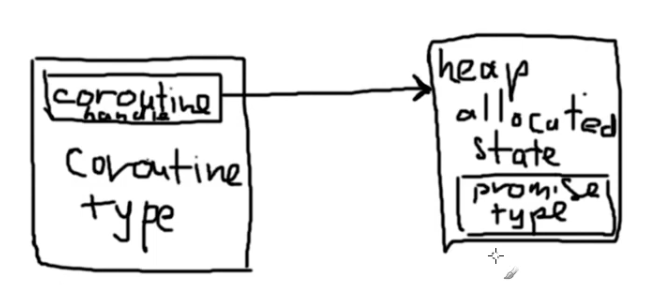
\includegraphics[scale=0.7]{coroutines.png}\\
Вот пример, как мог бы выглядеть изнутри класс генератора:
\begin{minted}[tabsize=4, autogobble]{C++}
	template <typename T>
	struct generator_promise;
	
	template <typename T>
	struct generator {
		using promise_type = generator_promise<T>;
		
		generator() = delete;
		generator(std::coroutine_handle<promise_type> handle)
		: handle(handle)
		{}
		
		generator(generator const&) = delete;
		generator& operator=(generator const&) = delete;
		
		~generator() {
			handle.destroy();
		}
		
		std::optional<T> next() {
			handle.resume();
			if (handle.done())
				return std::nullopt;
			
			return *handle.promise().currently_yielded_value;
		}
		
		private:
		std::coroutine_handle<promise_type> handle;
	};
	
	template <typename T>
	struct generator_promise {
		generator<T> get_return_object() noexcept {
			return generator<T>(
			std::coroutine_handle<generator_promise>::from_promise(*this)
			);
		}
		
		std::suspend_always yield_value(T const& value) noexcept {
			currently_yielded_value = &value;
			return {};
		}
		
		T const* currently_yielded_value;
	};
\end{minted}
Теперь разберемся, как работают вызовы корутины. Операция co\textunderscore yield на самом деле переписывается в другую:
\begin{minted}[tabsize=4, autogobble]{C++}
	// co_yield <expr>;
	
	// co_await promise.yield_value(expr);
\end{minted}
Операция, которая передается в await называется awaitable. Помимо yield value к ним относятся всякие асинхронные read и write. С await компилятор работает следующим образом. Сначала с помощью функции await\textunderscore ready проверяется, готовы ли данные, на тот случай, если awaitable вернет что-то сразу. В противном случае вызывается функция await\textunderscore suspend, которой передается хэндл корутины. Эта функция говорит корутине заснуть, пока функция не будет готова. Когда функция готова, вызывается await\textunderscore resume, который достает возвращаемое значение. Есть два особых awaitable: suspend\textunderscore never и suspend\textunderscore always. Первый всегда готов, а второй вечно спит. У корутины может быть два варианта поведения: она может после создания дойти до первой точки останова и там остановиться, либо просто зайти в фигурную скобку и остановиться. Мы хотим от генератора, чтобы он при создании не пошел сразу считать первое значение, а выбрал второй вариант поведения. У promise для этого есть метод initial\textunderscore suspend, который вызывается в начале co\textunderscore await. Аналогично в конце вызывается final\textunderscore suspend. Еще есть return\textunderscore void и unhandled\textunderscore expression. Их тоже нужно указывать при создании класса promise.\\
\textit{Замечание.} Не пользуйтесь обычным генератором для рекурсивных корутин. Используйте recursive\textunderscore generator.\\
\par Между stackful и stackless корутинами есть довольно много различий. Во-первых, с точки зрения stackful корутин любая функция может быть корутиной, а с точки зрения stackless нужно думать, прежде чем ставить куда-то await. Еще stackful, очевидно, использует стеки или segmented стеки (маленькие кусочки), а stackless выделяет память динамически.\\

\includegraphics[scale=0.6]{pop_cat.png}
\end{document}
